% !TEX TS-program = pdflatexmk
\documentclass[12pt,a4paper,header]{abnt}

\usepackage[brazilian]{babel}        
\usepackage[utf8]{inputenc} 

\usepackage[hypertexnames=false]{hyperref}
\usepackage{bookmark}
\usepackage{amsmath,amssymb,amsfonts}
\usepackage{graphicx}
\usepackage{subfigure}
\usepackage{fancyhdr}
\usepackage{array}
\usepackage{booktabs}
\usepackage{longtable}
\usepackage{xltabular}
\usepackage{float}

\usepackage{pdfpages} % Acrescentar pdf ficha bibliográfica

\usepackage[alf]{abntex2cite}	% Citações padrão ABNT

\usepackage{verbatim} % para comentários em blocos

\usepackage{textcomp}
\usepackage[T1]{fontenc}

\newcolumntype{L}[1]{>{\raggedright\arraybackslash}p{#1}}

%%%%%%%%%%%%%%%%%%%%%%%%%%%
%Teoremas, definicoes, etc%
%%%%%%%%%%%%%%%%%%%%%%%%%%%

\newtheorem{thm}{Teorema}[chapter]
\newtheorem{cor}{Corolário}[chapter]
\newtheorem{lem}{Lema}[chapter]
\newtheorem{defi}{Definição}[chapter]
\newtheorem{exe}{Exemplo}[chapter]
\newtheorem{prop}{Proposição}[chapter]

\renewcommand{\ABNTchapterfont}{\bfseries}
\renewcommand{\ABNTsectionfont}{\bfseries}

\fancypagestyle{logouff}{%
	\renewcommand{\headrulewidth}{0pt}
	\fancyhead{}
	\fancyhead[R]{
\includegraphics[width=0.7\textwidth]{assets/logoUFF.pdf}}% Your logo/image
  	\setlength{\headheight}{30pt} 
  	\setlength{\headsep}{2cm}
}

\hbadness=10000
\hfuzz=40pt
\vfuzz=20pt

\renewcommand{\topfraction}{0.85}
\renewcommand{\bottomfraction}{0.80}
\renewcommand{\textfraction}{0.15}
\renewcommand{\floatpagefraction}{0.75}

%%%%%%%%%%%%%%%%%%%%%%%%%%%%%%%%%%%%%%%%%%%%%%%%%%%%%%%%
% Macros dinamicas geradas em ../output/            %
%  criado para permitir caminho sem espacos no TeX)    %
%%%%%%%%%%%%%%%%%%%%%%%%%%%%%%%%%%%%%%%%%%%%%%%%%%%%%%%%
\graphicspath{{../output/figures/}{assets/}}
% Macros dinâmicas geradas por 04_analises_descritivas.R - nao editar manualmente
\newcommand{\NumMunicipios}{5.564}
\newcommand{\PeriodoEstudo}{2010 a 2025}
\newcommand{\TotalCasosProvaveis}{22.187.924}
\newcommand{\TotalObitos}{16.975}
\newcommand{\Letalidade}{0,08\%}
\newcommand{\TIAccumBrasil}{10.780,9}
\newcommand{\CasosDoisMilVinteQuatro}{6.433.460}
\newcommand{\TIDoisMilVinteQuatro}{3.026,4}
\newcommand{\CasosDoisMilVinteCinco}{1.636.855}
\newcommand{\PctSexoFeminino}{54,9\%}
\newcommand{\PctSexoMasculino}{44,9\%}
\newcommand{\PctFaixaZeroAQuatro}{2,6\%}
\newcommand{\PctFaixaVinteATrintaNove}{36,8\%}
\newcommand{\PctFaixaSessentaMais}{11,9\%}
\newcommand{\TempMaxBrasil}{34,6\textdegree C}
\newcommand{\UmidMediaBrasil}{73,6\%}
\newcommand{\PrecipAnualBrasil}{1.304 mm}
\newcommand{\PropAguaRedeBrasil}{83,9\%}
\newcommand{\PropEsgotoRedeBrasil}{64,7\%}
\newcommand{\PropLixoBrasil}{91,7\%}
\newcommand{\PropFavelaBrasil}{8,2\%}
\newcommand{\MediaMunAgua}{71,7\%}
\newcommand{\MediaMunEsgoto}{37,7\%}
\newcommand{\MediaMunLixo}{80,2\%}
\newcommand{\MediaMunFavela}{1,0\%}
\newcommand{\PctMunAltoRisco}{93,4\%}
\newcommand{\PctMunMedioRisco}{4,6\%}
\newcommand{\PctMunBaixoRisco}{2,0\%}
\newcommand{\PctMunPersistencia}{12,2\%}
\newcommand{\MoranMin}{0,215}
\newcommand{\MoranMax}{0,613}
\newcommand{\MoranDoisMilVinteQuatro}{0,613}
\newcommand{\TIRegiaoCentroOeste}{1.295,5}
\newcommand{\TIRegiaoSudeste}{897,5}
\newcommand{\TIRegiaoSul}{595,2}
\newcommand{\TIRegiaoNordeste}{325,4}
\newcommand{\TIRegiaoNorte}{265,4}

% Macros dinamicas geradas por 04_analises_descritivas.R
\newcommand{\LisaHH}{857}
\newcommand{\LisaLL}{1.324}
\newcommand{\LisaHL}{12}
\newcommand{\LisaLH}{29}
\newcommand{\LisaNS}{3.342}
\newcommand{\LisaSig}{2.222}
\newcommand{\LisaPctHH}{15,4\%}
\newcommand{\LisaPctLL}{23,8\%}
\newcommand{\LisaPctHL}{0,2\%}
\newcommand{\LisaPctLH}{0,5\%}
\newcommand{\LisaPctNS}{60,1\%}
\newcommand{\LisaPctSig}{39,9\%}

% Modelo canônico reportado: varredura puramente espacial.
% Macros dinamicas geradas por 05_varredura_satscan.R - nao editar manualmente
\newcommand{\ScanTotalCasos}{22.098.006}
\newcommand{\ScanPopulacao}{204.973.525}
\newcommand{\ScanNumMunicipios}{5.564}
\newcommand{\ScanB}{999}
\newcommand{\ScanSemente}{12345}
\newcommand{\ScanJanelaPop}{16\%}
\newcommand{\ScanRaioMaxKm}{200}
\newcommand{\ScanNumClusters}{129}
\newcommand{\ScanPrimID}{1}
\newcommand{\ScanPrimPolo}{Adolfo}
\newcommand{\ScanPrimUF}{São Paulo}
\newcommand{\ScanPrimMunicipios}{319}
\newcommand{\ScanPrimRaioKm}{197,4}
\newcommand{\ScanPrimCasosObs}{2.342.103}
\newcommand{\ScanPrimCasosEsp}{842.629}
\newcommand{\ScanPrimRR}{2,99}
\newcommand{\ScanPrimPValor}{< 0,001}
\newcommand{\ScanPrimLLR}{948.987}
\newcommand{\ScanPrimPop}{7.815.934}
\newcommand{\ScanPrimPopPct}{3,8\%}
\newcommand{\ScanPrimCasosPct}{10,6\%}
\newcommand{\ScanCobMunicipios}{1.907}
\newcommand{\ScanCobMunicipiosPct}{34,3\%}
\newcommand{\ScanCobCasos}{14.175.688}
\newcommand{\ScanCobCasosPct}{64,1\%}
\newcommand{\ScanCobCasosEsp}{6.623.049}
\newcommand{\ScanCobPop}{61.433.127}
\newcommand{\ScanCobPopPct}{30,0\%}
\newcommand{\ScanMaxRR}{4,95}
\newcommand{\ScanMaxRRPolo}{Cruzeiro do Sul}
\newcommand{\ScanMaxRRUF}{Acre}
\newcommand{\ScanMaxRRCasos}{46.111}
\newcommand{\ScanMaxRRMun}{1}
\newcommand{\ScanWmape}{75,1}
\newcommand{\ScanSecID}{2}
\newcommand{\ScanSecPolo}{Araújos}
\newcommand{\ScanSecUF}{Minas Gerais}
\newcommand{\ScanSecMunicipios}{229}
\newcommand{\ScanSecRaioKm}{199,8}
\newcommand{\ScanSecCasosObs}{2.588.779}
\newcommand{\ScanSecCasosEsp}{1.019.064}
\newcommand{\ScanSecRR}{2,74}
\newcommand{\ScanSecPValor}{< 0,001}
\newcommand{\ScanTerID}{3}
\newcommand{\ScanTerPolo}{Palmelo}
\newcommand{\ScanTerUF}{Goiás}
\newcommand{\ScanTerMunicipios}{122}
\newcommand{\ScanTerRaioKm}{198,1}
\newcommand{\ScanTerCasosObs}{2.259.957}
\newcommand{\ScanTerCasosEsp}{948.039}
\newcommand{\ScanTerRR}{2,54}
\newcommand{\ScanTerPValor}{< 0,001}

% Macros geradas por 04b_heatmap_uf_ano.R - nao editar manualmente
\newcommand{\TIMaxUF}{DF}
\newcommand{\TIMaxUFAno}{2024}
\newcommand{\TIMaxTI}{9.298,2}
\newcommand{\TIMinUF}{ES}
\newcommand{\TIMinUFAno}{2021}
\newcommand{\TIMinTI}{0,8}


\begin{document}

%%%%%%%%%%%%%%%%%%%%%%%%%%%%%%
%colocar aqui o nome do aluno%
%%%%%%%%%%%%%%%%%%%%%%%%%%%%%%
\autor{Lucas Batista de Oliveira}


%%%%%%%%%%%%%%%%%%%%%%%%%%%%%%%%%%%%%
%colocar aqui o título da monografia%
%%%%%%%%%%%%%%%%%%%%%%%%%%%%%%%%%%%%%
\titulo{Distribuição espacial da dengue no Brasil: identificação de áreas de alto risco e características socioambientais}


%%%%%%%%%%%%%%%%%%%%%%%%%%%%%%%%%%%
%colocar aqui o nome do orientador%
%%%%%%%%%%%%%%%%%%%%%%%%%%%%%%%%%%%
\orientador{Prof. Dr. Rafael Santos Erbisti}  


%%%%%%%%%%%%%%%%%%%%%%%%%%%%%%%%%%%%%%%%%%%%%%%%%%%%
%colocar aqui o nome do co-orientador, caso exista%%
%se nao existir, comente a linha de codigo a seguir%
%ATENCAO: se nao houver co-orinetador também deve  %
%         ser comentada a linha 124, onde aparece  %
%         "Co-Orientador: & \ABNTcoorientadordata" %
%%%%%%%%%%%%%%%%%%%%%%%%%%%%%%%%%%%%%%%%%%%%%%%%%%%%
%\coorientador{Prof. Dr. Nome do Co-orientador}


%%%%%%%%%%%%%%%%%%%%%%%%%%%%%%%%%%%%%%%%%%%%%%%%%%%
%colocar aqui a data da apresentacao da monografia%
%segue um exemplo								  %
%%%%%%%%%%%%%%%%%%%%%%%%%%%%%%%%%%%%%%%%%%%%%%%%%%%
\data{13 de novembro de 2026}

%%%%%%%%%%%%%%%%%%%%%%%%%%%
%nao mexer até a linha 170%
%%%%%%%%%%%%%%%%%%%%%%%%%%%

\comentario{Monografia apresentada para obtenção do grau de Bacharel em Estatística pela Universidade Federal Fluminense.}

\instituicao{Departamento de Estatística \par Instituto de Matemática e Estatística \par Universidade Federal Fluminense}

\local{Niterói - RJ, Brasil}

\capa

\vspace{10cm}



\begin{titlepage}

\thispagestyle{logouff}

\vspace{2cm}

\hspace{.2\textwidth} % posicionando a minipage
\begin{minipage}{.7\textwidth}

\begin{flushright}

{\large \bf \ABNTautordata} \\[3cm]

{\Large \bf \ABNTtitulodata}\\[3cm]

{\bf Trabalho de Conclusão de Curso}\\[1cm]

\end{flushright}

\begin{espacosimples}

\ABNTcomentariodata

\end{espacosimples}

\vspace{1cm}

\hfill 
\begin{tabular}{rl}
Orientador(a): & \ABNTorientadordata\\
%%%%%%%%%%%%%%%%%
% Comentar linha seguinte caso não haja co-orientador
% Co-Orientador(a): & \ABNTcoorientadordata
\end{tabular}

\end{minipage}

\vspace{7cm}

\begin{center}

\ABNTlocaldata

\ABNTdatadata

\end{center}

\end{titlepage}


%folha de aprovacao com as assinaturas - Editar os membros da banca
\begin{folhadeaprovacao}

\thispagestyle{logouff}

\hspace{.2\textwidth} % posicionando a minipage
\begin{minipage}{.7\textwidth}

\begin{flushright}

{\large \bf \ABNTautordata}\\[1cm]

{\large \bf \ABNTtitulodata}\\[1cm]

\end{flushright}
Monografia de Projeto Final de Graduação sob o título \textit{``\ABNTtitulodata''},
defendida por \ABNTautordata~e aprovada em \ABNTdatadata, na cidade de Niterói,
no Estado do Rio de Janeiro, pela banca examinadora constituída pelos
professores:
\begin{flushright}

\begin{espacosimples}

%Folha de assinaturas
%%%%%%%%%%%%%%%%%%%%%%%%%%%%%%%%%%%%%%%%%
%Preencher os dados dos membros da banca%
%%%%%%%%%%%%%%%%%%%%%%%%%%%%%%%%%%%%%%%%%

\vspace{1.5cm}
\noindent\rule{10cm}{0.4pt}\\
{\bf Prof. Dr. Rafael Santos Erbisti}\\
Departamento de Estatística, UFF\\

%se o trabalho não tiver co-orientator, comentar as 4 linhas que seguem
%\vspace{1.5cm}
%\noindent\rule{10cm}{0.4pt}\\
%{\bf Prof. Dr. Nome do Co-Orientador}\\
%Departamento de Estatística, UFF\\


\vspace{1.5cm}
\noindent\rule{10cm}{0.4pt}\\
{\bf Prof. Dr. Guilherme Augusto Veloso}\\
Departamento de Estatística, UFF \\

\vspace{1.5cm}
\noindent\rule{10cm}{0.4pt}\\
{\bf Dra. Nildimar Alves Honório}\\
LIVH/IOC, Fiocruz \\

%\vspace{1.5cm}
%\noindent\rule{10cm}{0.4pt}\\
%{\bf Profa. Ma. Nome do 2º membro da banca}\\
%Instituição do 2º membro da banca\\

\end{espacosimples}

\end{flushright}

\vspace{1.5cm}
\hfill Niterói, \ABNTdatadata

\end{minipage}

\end{folhadeaprovacao}

%%%%%%%%%%%%%%%%%%%%%%%%%%%%%%%%%%%%%%%%%%%%%%%%%%%%%%%%%%%%
% inclusão de ficha bibliográfica
% retire o símbolo de comentário e corrija o nome do arquivo
%%%%%%%%%%%%%%%%%%%%%%%%%%%%%%%%%%%%%%%%%%%%%%%%%%%%%%%%%%%%

%\includepdf[pages=-]{ficha.pdf}

%%%%%%%%%%%%%%%%%%%%%%%%%%%%%%%%%%%%%%%
%escreva aqui o resumo do seu trabalho%
%%%%%%%%%%%%%%%%%%%%%%%%%%%%%%%%%%%%%%%
\begin{resumo}
Este estudo descreve a distribuição espacial do risco de dengue no Brasil entre 2010 e 2025 e avalia como a delimitação de zonas de alto risco varia segundo a padronização indireta por covariáveis e a exclusão de 2024. Analisaram-se 22.098.006 casos prováveis em um painel de 5.564 municípios harmonizados à malha de 2010. Foram realizadas análises descritivas, de autocorrelação espacial global e local e de varredura espacial de Kulldorff, com modelo discreto de Poisson, em oito formulações: uma sem ajuste e sete com padronização indireta por covariáveis climáticas, de saneamento e de urbanização. A varredura utilizou janela circular limitada a 16\% da população sob risco e a 200 km de raio, 999 réplicas de Monte Carlo e reporte hierárquico a 5\% sem sobreposição geográfica. O Índice Global de Moran foi positivo e estatisticamente significativo nos 16 anos (0,215–0,613). As zonas de alto risco concentraram-se no Centro-Sul, sobretudo no Sudeste e Centro-Oeste. Sem ajuste, foram identificadas 129 zonas, que reuniram 64,1\% dos casos e 30,0\% da população sob risco; a zona primária, centrada em Adolfo (SP), abrangia 319 municípios (RR = 2,99). Nos sete ajustes, o número de zonas variou de 128 a 195 e o WMAPE de 64,9\% a 74,4\%, ante 75,1\% sem ajuste. A exclusão de 2024 alterou o número de zonas em todas as formulações e o polo primário em sete. A distribuição apresentou estrutura espacial, mas a delimitação das zonas variou segundo a padronização e o período. As comparações são exploratórias e não permitem inferir efeitos causais das covariáveis.

\vspace{1cm}
\noindent Palavras-chave: Estatística Espacial. Varredura Espacial. Índice de Moran. Agrupamentos Espaciais. Dengue.

\end{resumo}

\begin{abstract}
This study describes the spatial distribution of dengue risk in Brazil from 2010 to 2025 and assesses how high-risk zone delineation varies with indirect covariate standardization and exclusion of 2024. We analyzed 22,098,006 probable cases in a panel of 5,564 municipalities harmonized to the 2010 municipal grid. Descriptive, global and local spatial autocorrelation, and Kulldorff spatial scan analyses were conducted using a discrete Poisson model and eight formulations: one unadjusted and seven indirectly standardized by climate, sanitation and urbanization covariates. The scan used a circular window limited to 16\% of the population at risk and a 200-km radius, 999 Monte Carlo replications, and hierarchical reporting at the 5\% level without geographic overlap. Global Moran's I was positive and statistically significant in all 16 years (0.215–0.613). High-risk zones were concentrated in the Center-South, especially in the Southeast and Center-West. The unadjusted scan identified 129 zones, containing 64.1\% of cases and 30.0\% of the population at risk; the primary zone, centered on Adolfo, São Paulo, comprised 319 municipalities (RR = 2.99). Across the seven adjusted formulations, the number of zones ranged from 128 to 195 and WMAPE from 64.9\% to 74.4\%, compared with 75.1\% without adjustment. Excluding 2024 changed the number of zones in all formulations and the primary cluster location in seven. Spatial structure was observed, but zone delineation varied with covariate standardization and study period. These comparisons are exploratory and do not support causal inference about the covariates.

\vspace{1cm}
\noindent Keywords: Spatial Statistics. Spatial Scan Statistics. Moran's I. Spatial Clusters. Dengue.

\end{abstract}



%%%%%%%%%%%%%%%%%%%%%%%%%%%%%%%%
%escreva aqui a sua dedicatória% (opcional)
%%%%%%%%%%%%%%%%%%%%%%%%%%%%%%%%

\chapter*{Dedicatória}
Dedico esta obra, cuja serventia científica ainda não conheço, a mim mesmo. Todo o apoio que me foi dado serviu para que eu não desistisse, mas o caminho foi trilhado por mim, sem que outra pessoa pudesse percorrê-lo em meu lugar.  



%%%%%%%%%%%%%%%%%%%%%%%%%%%%%%%%%%
%escreva aqui seus agradecimentos% (opcional)
%%%%%%%%%%%%%%%%%%%%%%%%%%%%%%%%%%
\chapter*{Agradecimentos}

A Deus, sobretudo, e a todos os santos, os quais roguei por intercessão talvez menos do que deveria. Em especial, Santa Rita dos Impossíveis, cujo milagre, tal qual um grão, deu um fruto: este fruto.

A Ana Beatriz Monteiro Fonseca, a Bia, que olhou para mim com fé e bondade, e que me levou ao caminho que percorro até hoje, com alegria e gratidão. Ainda hoje conto com seus direcionamentos e ouço atentamente seu falar, porque é sobre a luz que ela fala, e sob a luz eu quero ficar. Jamais esquecerei o que fizeste por mim, minha querida amiga, e o fizeste com amor. Torno público, aqui, meu contrato eterno de gratidão a ti.

Ao meu amado mestre, Rafael Santos Erbisti, pelas caronas, almoços e jantares, conversas e companhia, paciência, brincadeiras, e tudo o que era permitido viver a cada encontro presencial ou remoto. Por ter dado a mim espaço e voz, mas também conselhos e advertências, afinal, se não há crescimento sem estímulo, também não há sem disciplina. Por ter acreditado em si mesmo e não ter desistido do que sempre quis para si, tornando-se, hoje, uma referência para quem longe ou perto está. Não posso deixar de mencionar sua importância para o curso que hoje estou a me formar: seus feitos elevaram nosso patamar. Você é um ser iluminado.

A Ana Maria Lima de Farias, por sua competência como docente e administradora, que fez do local onde passei mais de 4 anos da vida um verdadeiro campo de conquistas e, também, a Jessica Quintanilha Kubrusly, que me introduziu à vida científica de maneira sublime e que construiu parte do ser que hoje escreve este texto.

A criatura divina, que não ouso cometer o pecado de chamar apenas de amigo, Yan Breno Azeredo Gomes da Silva. Esse trabalho de conclusão de curso finda o percurso que fiz por longos anos, sob diversas intempéries, nas quais sempre estivemos juntos: só nós dois sabemos como é vir do nada e chegar aqui. Para além disso, aqui, também, é findada a construção do patamar de apoio para os próximos passos, cuja direção é a contribuição social efetiva que tanto sonhamos. Sua trajetória, meu camarada, me inspira diariamente; e é na excelência que presencio que quero chegar. Tens todo o meu carinho e admiração!

Por fim, se devo gratidão a esse tanto de gente estranha, quem dirá à minha família, sobretudo, meus pais: Rose e Inácio. Meu eu no passado jamais ousaria vislumbrar a luz de um dia futuro sem que, do momento da descoberta da gestação que me trouxe ao mundo até o presente dia da marcha de minha história, tivessem firmado um contrato de responsabilidade caro, longo e sem garantia de benefícios. No que me formo em breve (assim espero!), talvez eles não tenham noção. No entanto, mesmo não sabendo, olham para mim e dizem: "que orgulho de você, meu filho". Mesmo que eu saiba que o futuro nos reserva uma coexistência inexistente, escrevo isso sob lágrimas e desespero. Até o meu último dia nessa terra feroz, triste e que marcha rumo a uma situação inóspita, darei meu melhor por vocês e pelo futuro de meu irmão. Obrigado. Da alma, obrigado.
\tableofcontents{}
\listoffigures
\listoftables


%%%%%%%%%%%%%%%%%%%%%%%%%%%%%%%%%%%%%%%%%%%%
%Aqui começam os capítulo da sua monografia%
%%%%%%%%%%%%%%%%%%%%%%%%%%%%%%%%%%%%%%%%%%%%


\chapter{Introdução}
\label{cap:introducao}

As arboviroses transmitidas por \textit{Aedes aegypti} e \textit{Aedes albopictus}, em especial dengue (DENV), chikungunya (CHIKV) e Zika (ZIKV), estão entre as principais ameaças à saúde pública global \cite{gould2017}. Estima-se que 5,66 bilhões de pessoas vivam em áreas ambientalmente adequadas à transmissão de dengue, chikungunya e Zika, com subnotificação acentuada em regiões de baixa vigilância \cite{lim2025a}. Entre elas, a dengue é a de maior magnitude epidemiológica nas Américas, onde o número de casos cresceu de forma acentuada na última década, com epidemias recorrentes e expansão territorial da doença \cite{lim2025a,parums2025}. O impacto sanitário é elevado, com estimativas globais da ordem de 390 milhões de infecções anuais, além de morbidades crônicas e sobrecarga frequente dos sistemas de saúde \cite{parums2025}.

Fatores ecológicos e sociais se reforçam mutuamente. Mudanças climáticas alteram a distribuição dos vetores, favorecendo a expansão de áreas adequadas à transmissão. Sob cenários de aquecimento mais intenso, projeções indicam mais população exposta em diferentes regiões do mundo \cite{ryan2019}. Revisões sistemáticas mostram co-distribuição entre baixa escolaridade, precariedade habitacional, interrupções no abastecimento de água e maior vulnerabilidade à infecção em áreas urbanas densas \cite{power2022}. A dengue varia no espaço conforme o contexto ambiental e socioeconômico.

No Brasil, a circulação simultânea das três arboviroses caracteriza o período recente. Em 11 de novembro de 2015, o Ministério da Saúde declarou Emergência em Saúde Pública de Importância Nacional diante da alteração do padrão de ocorrência de microcefalias; a associação epidemiológica com a infecção congênita pelo vírus Zika foi descrita posteriormente. A série histórica do Ministério da Saúde, atualizada até a Semana Epidemiológica 47 de 2023, registra 213.350 casos prováveis de Zika em 2016 \cite{portaria1813,ms_zika}. Apenas em 2016, dengue, chikungunya e Zika geraram gastos da ordem de R\$ 2,3 bilhões \cite{2018-teich-arinelli-fahham}. A dengue concentrou o maior volume de casos e a dispersão territorial mais ampla, presente em quase todos os municípios do país \cite{pescarini2022}.

O Informe Semanal nº 18 do Ministério da Saúde, atualizado em 11 de junho de 2024, registrou 5.831.871 casos prováveis até a Semana Epidemiológica 23 e incidência de 2.872,0 por 100 mil habitantes; no mesmo recorte de 2023, a incidência era de 627,9 por 100 mil \cite{ms_informe2024}. Em 4 de dezembro de 2024, dados do painel ministerial reportados pela Agência Brasil indicavam 6.590.575 casos prováveis e incidência de 3.245 por 100 mil habitantes; esse valor é uma fotografia publicada naquela data, não o fechamento final do ano \cite{agenciabrasil_dengue2024}.

Muitos estudos avaliam os padrões de dengue e das demais arboviroses em escalas espaciais menores, e a cidade e o estado do Rio de Janeiro estão entre os territórios mais documentados no país. No Rio de Janeiro, estudos identificaram soroprevalência elevada para as três arboviroses e concentração de casos em áreas socialmente mais vulneráveis \cite{2023-souza-santos-sobral-perisse}. No município do Rio de Janeiro, a incidência das arboviroses concentra-se em espaços com piores indicadores socioeconômicos \cite{2021-queiroz-medronho}; na região Norte, a incidência de dengue acompanha vulnerabilidade social e urbanização \cite{2023-gomes-jesus-quaresma}. Essa heterogeneidade no espaço fundamenta a identificação de áreas de maior risco.

A heterogeneidade espacial e temporal orienta a estratificação de risco para a vigilância e o controle das arboviroses. Mapas de risco e detecção de agrupamentos espaciais fornecem informação territorial para o planejamento da vigilância e das ações de controle \cite{parums2025,liu2025}. Revisões da literatura apontam que a evidência disponível sobre a efetividade de diferentes intervenções de controle vetorial ainda é limitada \cite{bowman2016}.

Na literatura, a análise espacial da dengue e de outras arboviroses passou de abordagens descritivas para modelagens mais complexas. Estudos iniciais usaram índices de autocorrelação espacial, como o Índice de Moran \cite{moran1950,anselin1995}, para medir a dependência geográfica da doença em nível municipal e intramunicipal. \citeonline{almeida2009}, por exemplo, descreveram a concentração de casos na Zona Oeste do Rio de Janeiro, associada à falta de infraestrutura sanitária geral.

Em escalas distintas, \citeonline{rodrigues2018} e \citeonline{vernal2021} mapearam a variação espacial da incidência em comunidades vulneráveis e em municípios paulistas. Os resultados indicaram que indicadores estruturais básicos não bastavam para descrever a heterogeneidade da transmissão, que variava também com características sociodemográficas e geoclimáticas.

\citeonline{lowe2011} usaram modelos estatísticos baseados em anomalias climáticas sazonais para construir sistemas de alerta precoce. O efeito das temperaturas extremas e das chuvas na incidência e na dinâmica epidêmica foi analisado por meio de séries temporais e modelos espaço-temporais em diferentes regiões endêmicas \cite{xavier2021, ribeiro2025, alves2025}.

Em escala nacional, análises espaço-temporais associaram o risco de dengue a extremos hidrometeorológicos e à urbanização, incluindo mudanças na distribuição da doença em regiões do Sul e da Amazônia \cite{lee2021, lowe2021}. Modelos de difusão indicam maior adequação ambiental para mosquitos vetores em áreas temperadas da Europa \cite{barman2025}, enquanto a mortalidade segue concentrada em populações socialmente vulneráveis \cite{cardim2025}.

Para delimitar \textit{clusters} de alto risco, o método de Kulldorff tem sido usado para detectar \textit{clusters} espaço-temporais e rotas de disseminação de dengue, Zika e chikungunya, em contextos internacionais \cite{freitas2022} e no território nacional. No Brasil, \citeonline{palasio2023} investigaram \textit{clusters} espaço-temporais de Zika e chikungunya; \citeonline{almeida2023} identificaram \textit{clusters} simultâneos para as três arboviroses no estado do Rio de Janeiro, com vulnerabilidade persistente de regiões metropolitanas centrais; e revisões do cenário nacional tratam a dengue como desafio endêmico contínuo \cite{2020-magalhaes-et-al}.

Comparações entre as janelas circular e flexível indicam desempenho similar, com tendência da circular a delimitar áreas maiores e da flexível a delimitar áreas menores \cite{melo2022}. Ajustes no teto populacional refinam a sensibilidade da vigilância local \cite{canal2017}.

Esses métodos foram aplicados sobretudo em recortes territoriais específicos ou em períodos delimitados. Estudos sobre a expansão da dengue no Brasil descrevem ondas de difusão de regiões metropolitanas para cidades médias e pequenas, condicionadas por clima, população e conectividade \cite{barcellos2014}. Persiste, assim, uma lacuna de trabalhos que apliquem a varredura espacial de forma contínua a todo o território nacional por um período longo, com dados recentes, e que comparem o efeito de diferentes estratificações sobre a geografia dos excessos. O presente trabalho busca preencher essa lacuna ao cobrir os 5.564 municípios da malha de 2010 em 16 anos, de 2010 a 2025, incluindo o ano epidêmico de 2024, e ao contrapor oito formulações da mesma varredura, com e sem padronização indireta. O acompanhamento contínuo de toda a extensão do país viabiliza captar as dinâmicas de interiorização e a evolução temporal da doença, oferecendo subsídios para uma compreensão de conjunto do agravo.

Nesse sentido, o objetivo geral deste trabalho é descrever a distribuição espacial do risco de dengue no Brasil entre 2010 e 2025. Os objetivos específicos são descrever a distribuição da doença em conjunto com variáveis ambientais, climáticas e sociais; identificar e delimitar zonas de alto risco em todo o território nacional; e avaliar como a geografia dessas zonas se altera quando a varredura controla diferentes conjuntos de covariáveis e quando o ano epidêmico de 2024 é retirado da série. As comparações com as covariáveis são descritivas e não são interpretadas como efeitos causais. Para delimitar as zonas, emprega-se a janela circular clássica, cujas extensões devem ser interpretadas com cautela.

Além desta Introdução, o texto está organizado em três capítulos. O Capítulo~\ref{cap:matmet} apresenta a área de estudo, as bases de dados, o tratamento das informações, as medidas de autocorrelação espacial, a estatística de varredura espacial e a comparação entre as formulações, além dos recursos computacionais empregados. O Capítulo~\ref{cap:resultados} traz os resultados descritivos, a caracterização socioespacial e climática, a autocorrelação espacial e a análise dos \textit{clusters}, com a comparação entre as formulações e a sensibilidade à exclusão de 2024. O Capítulo~\ref{cap:discussao} discute os achados e reúne as conclusões, as limitações e as perspectivas. Os apêndices complementam o texto com as tabelas completas de \textit{clusters} e as pranchas de mapas.


\chapter{Materiais e Métodos}
\label{cap:matmet}

Este capítulo descreve a área de estudo, as bases de dados utilizadas, o tratamento das informações, as medidas de autocorrelação espacial, a estatística de varredura espacial e a comparação entre as formulações, além dos recursos computacionais empregados e das definições descritivas adotadas.

\section{Área de Estudo}

O Brasil é o maior país da América do Sul em extensão territorial, com mais de 8,5 milhões de $km^2$, e possui população superior a 203 milhões de habitantes, segundo o último Censo Demográfico do Instituto Brasileiro de Geografia e Estatística (IBGE) \cite{ibge2022censo}. O território nacional está dividido administrativamente em 5.571 unidades territoriais\footnote{A divisão oficial vigente compreende 5.569 municípios, 1 Distrito Federal e 1 distrito estadual, totalizando 5.571 unidades. A malha de referência deste estudo baseia-se no Censo Demográfico de 2010, com 5.565 unidades; após a exclusão do distrito de Fernando de Noronha, o painel analisado contém 5.564 municípios, contando Brasília (DF) como município para a análise espacial.}, agrupadas em cinco grandes regiões: Norte, Nordeste, Centro-Oeste, Sudeste e Sul, como ilustrado na Figura~\ref{fig:mapa_regioes}. A Região Sudeste concentra a maior parte da população brasileira e responde por parcela substancial da atividade econômica nacional \cite{ibge2022atlas}.

Os biomas do país incluem Amazônia, Cerrado, Caatinga, Mata Atlântica, Pantanal e Pampa, distribuídos de forma heterogênea pelo território. O grau de urbanização é elevado, com grande parte da população em áreas urbanas. Densidade populacional, ocupação do território e condições de infraestrutura variam de forma expressiva entre municípios e regiões \cite{ibge2022atlas}.

\begin{figure}[H]
    \centering
    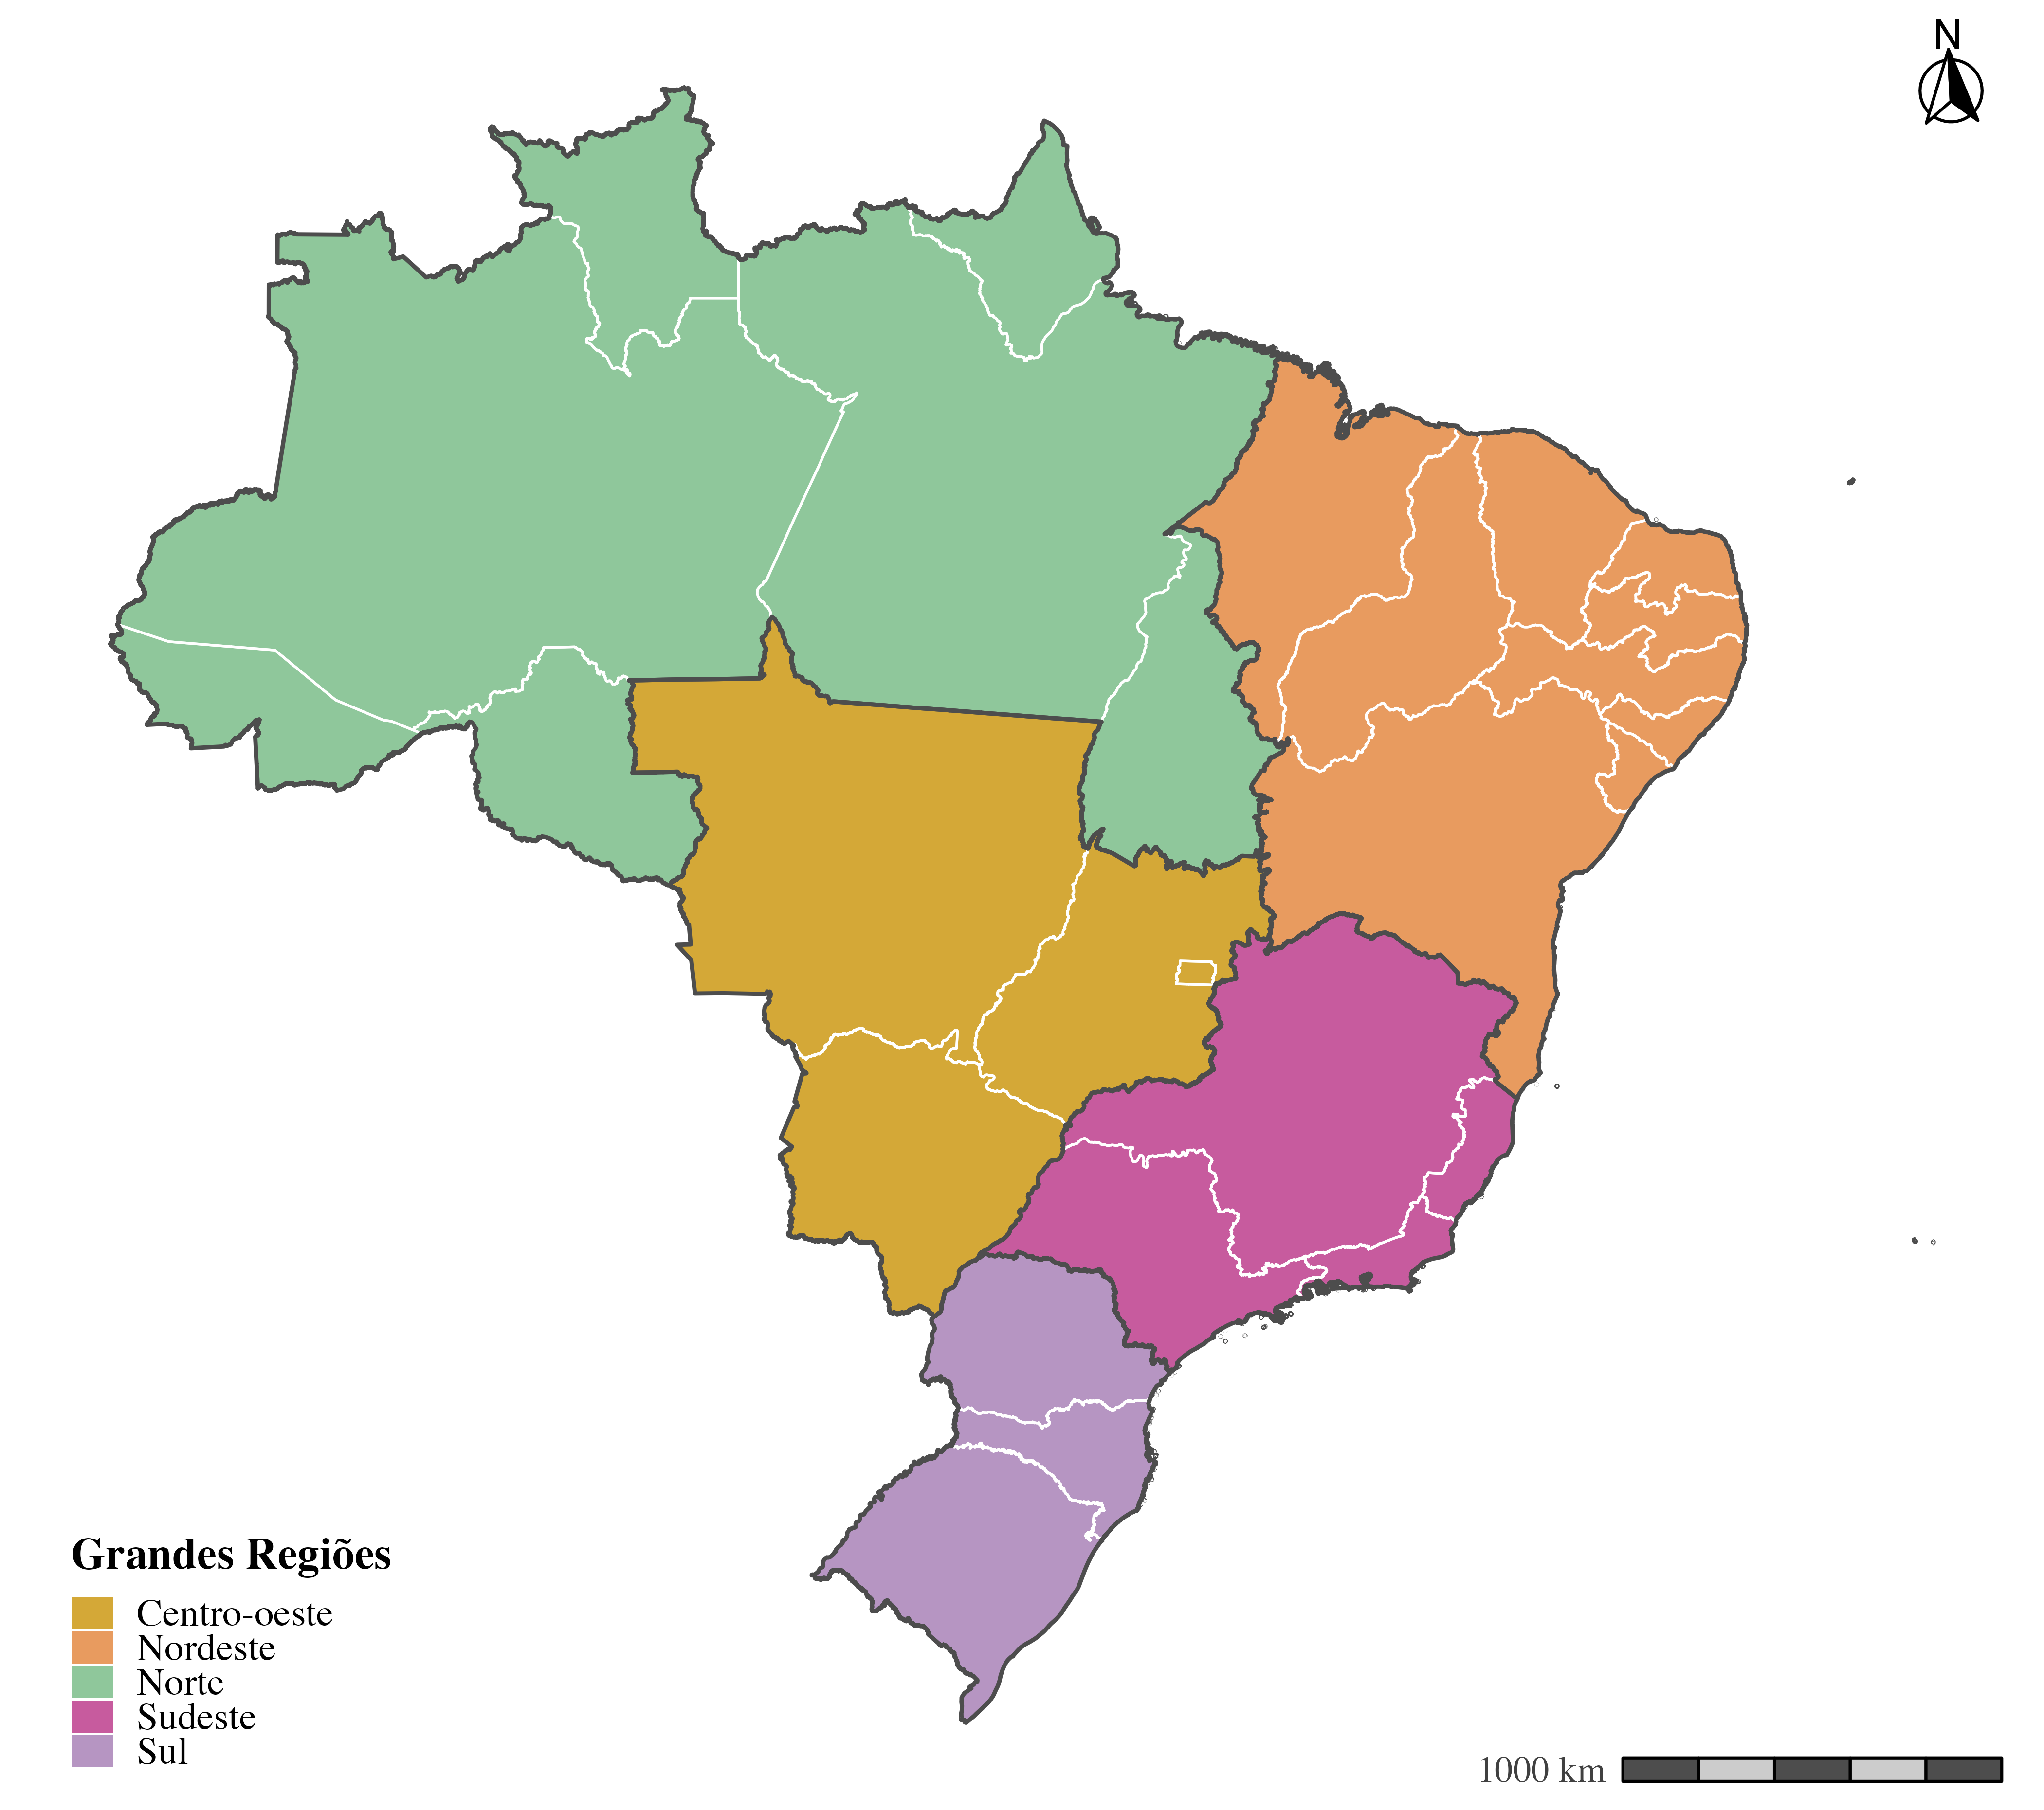
\includegraphics[width=0.76\textwidth]{fig_mapa_grandes_regioes.png}
    \caption{Divisão do território brasileiro por Grande Região. Fonte: IBGE.}
\label{fig:mapa_regioes}
    \vspace{0.3em}
    {\footnotesize\noindent\textit{Nota:} Divisão regional do IBGE; a malha municipal de análise segue a referência espacial de 2010.\par}
\end{figure}

\noindent \textbf{Grandes Regiões}

As características demográficas, territoriais e climáticas das grandes regiões vêm do Censo Demográfico 2022 \cite{ibge2022censo}, do Atlas Nacional do Brasil Milton Santos \cite{ibge2022atlas} e do Mapa de Clima do Brasil \cite{ibge2002clima}.

No Norte vivem aproximadamente 17,4 milhões de habitantes, com a menor densidade demográfica do país. Predomina a Floresta Amazônica, com grandes distâncias entre os principais centros urbanos. O clima é equatorial, com temperaturas elevadas, alta umidade e precipitação alta ao longo do ano.

Com cerca de 54,7 milhões de habitantes, o Nordeste contrasta a faixa litorânea, onde se concentram centros urbanos importantes, com o interior semiárido. Predominam climas tropicais, que variam com a proximidade do mar, a latitude e o relevo.

Aproximadamente 16,3 milhões de habitantes vivem no Centro-Oeste, em extensa área territorial com predomínio de Cerrado e Pantanal e baixa densidade demográfica. O clima é tropical sazonal, com períodos chuvosos e secos ao longo do ano.

O Sudeste, com cerca de 84,8 milhões de habitantes, tem urbanização elevada, forte integração entre áreas metropolitanas e participação expressiva na economia nacional. O clima varia entre tropical e subtropical, conforme latitude, relevo e altitude.

No Sul vivem aproximadamente 29,9 milhões de habitantes, concentrados sobretudo em áreas urbanas. O clima é subtropical, com estações mais definidas e médias de temperatura abaixo das demais regiões, além de integração territorial elevada e presença forte de centros urbanos de médio e grande porte.

\section{Bases de Dados}
\label{sec:bases_dados}

A unidade de análise é o município brasileiro, observado por ano civil, em um banco de dados longitudinal de \PeriodoEstudo{}. Todas as bases de informação — territoriais e populacionais, socioespaciais, climáticas e epidemiológicas — seguem essa mesma configuração, com escalas de observação do ano e do município.

\noindent \textbf{Dados territoriais e populacionais}

As estimativas populacionais anuais são oriundas do IBGE, com a seguinte disposição: 2010 a partir da malha censitária; 2011 a 2024 a partir das estimativas anuais fornecidas ao Tribunal de Contas da União (TCU), com exceção de 2011 e 2018, obtidos da tabela 6579 do Sistema IBGE de Recuperação Automática (SIDRA), devido a divergências pontuais de informações; 2025 a partir da tabela 6579 do SIDRA.

Considerando a extensão do recorte temporal (2010--2025), o território nacional passou por alterações em sua divisão político-administrativa, com a emancipação e criação de novos municípios. Para assegurar a consistência topológica e a comparabilidade longitudinal das métricas espaciais, adotou-se como referência fixa a malha vetorial municipal do Censo Demográfico de 2010, disponibilizada pelo IBGE, no sistema de referência SIRGAS 2000 (EPSG:4674). A harmonização espacial reatribuiu aos municípios de origem as estimativas populacionais e as notificações de casos dos municípios emancipados após 2010, antes de qualquer agregação. Foram aplicados cinco pares de reatribuição: Mojuí dos Campos para Santarém (PA), Pescaria Brava para Laguna (SC), Balneário Rincão para Içara (SC), Pinto Bandeira para Bento Gonçalves (RS) e Paraíso das Águas para Costa Rica (MS). Os demais códigos criados após 2010 seguiram a tabela de compatibilização pelo critério de maior área de sobreposição. Registros cujo código não pertence à malha de 2010 não encontram par na junção com o painel e, por isso, não são contados no painel espacial; a parcela residual não atribuível é quantificada nas Limitações deste trabalho.

O distrito estadual de Fernando de Noronha (PE) foi excluído da área de estudo, visto que sua condição de arquipélago oceânico impõe dinâmicas de contiguidade espacial e perfis epidemiológicos atípicos em relação ao território continental, o que poderia introduzir vieses na interpretação dos achados. Os 1.229 casos notificados no distrito no período foram igualmente excluídos do painel espacial. O estudo utiliza \NumMunicipios{} municípios\footnote{Nesta contagem, como prática em análises espaciais no país, Brasília (DF) foi considerada como município.}.

\noindent \textbf{Dados socioespaciais}

As variáveis socioespaciais descrevem saneamento básico e infraestrutura domiciliar: abastecimento de água, esgotamento sanitário e coleta de resíduos sólidos, além de densidade demográfica e proporção da população em favelas e comunidades urbanas, vindas do Censo Demográfico de 2022 (IBGE), via SIDRA \cite{ibge2022sidra}. Os valores do Censo 2022 são únicos por município e repetem-se nos 16 anos do painel, pois não há observações anuais dessas variáveis para o recorte temporal considerado\footnote{As informações censitárias de 2022 foram mantidas constantes nos demais anos do painel por indisponibilidade de medidas anuais comparáveis.}. As variáveis consideradas são apresentadas na Tabela~\ref{tab:variaveis_socioespaciais}. Para o esgotamento sanitário, adotou-se a definição de esgotamento adequado, que soma o acesso à rede coletora e à fossa séptica, em alinhamento com a divulgação oficial do IBGE. A área municipal em quilômetros quadrados foi calculada a partir da malha de 2010 projetada para EPSG:5880, dividindo-se a área em metros quadrados por um milhão. As proporções de água, esgoto e lixo usam como denominador o total de domicílios do município. A densidade demográfica e a proporção em favelas usam como base populacional a população residente apurada no recenseamento de 2022, e não as estimativas populacionais anuais: a primeira divide essa população pela área municipal, e a segunda divide a população em favelas pela população residente de 2022 e multiplica o resultado por cem. A tabela de favelas cobre 656 municípios com informação positiva e atribui valor zero aos demais.

\begin{table}[H]
\centering
\caption{Variáveis socioespaciais e demográficas consideradas no estudo.}
\label{tab:variaveis_socioespaciais}
\begin{tabular}{L{5cm} L{9cm}}
\hline
\textbf{Variável} & \textbf{Descrição} \\
\hline
Densidade demográfica &
Número de habitantes por quilômetro quadrado no município (Censo 2022). \\
\hline
Cobertura de abastecimento de água &
Proporção de domicílios com abastecimento de água por rede geral como forma principal (\%). \\
\hline
Cobertura de esgotamento sanitário &
Proporção de domicílios com esgotamento adequado, por rede geral/pluvial ou fossa séptica (\%). \\
\hline
Cobertura de coleta de resíduos sólidos &
Proporção de domicílios atendidos por serviço de coleta de lixo (direta ou caçamba) (\%). \\
\hline
População em favelas e comunidades urbanas &
Proporção da população residente em favelas e comunidades urbanas no município (\%). \\
\hline
\end{tabular}
\end{table}

\noindent \textbf{Dados climáticos}

As variáveis climáticas foram obtidas a partir de produtos de reanálise do \textit{European Centre for Medium-Range Weather Forecasts} (ECMWF), disponibilizados pelo \textit{Copernicus Climate Data Store} (CDS) \cite{copernicus_era5,copernicus_era5land}, para o período contínuo de 1º de janeiro de 2010 a 31 de dezembro de 2025.

Para a caracterização térmica diária, processou-se a série de reanálise de superfície (resolução espacial nativa de aproximadamente 9~km; grade regular de 0,1$^\circ$), com quatro observações diárias (00, 06, 12 e 18 UTC) por célula de grade. Os valores originais em Kelvin foram convertidos para graus Celsius. Assim, a máxima diária corresponde ao máximo dos quatro horários disponíveis, e não ao máximo horário contínuo. A extração para os municípios usou agregação ponderada pela área de interseção entre os polígonos dos 5.564 municípios da malha censitária de 2010 e as células da reanálise. Para cada município e dia da série, também foram calculadas a temperatura mínima e a média dos quatro horários.

A identificação de episódios de calor extremo foi parametrizada a partir da distribuição climatológica local. Para cada município, determinou-se o percentil 90 da distribuição empírica das temperaturas máximas diárias no período 2010--2025. Uma onda de calor foi definida operacionalmente como uma sequência de pelo menos três dias consecutivos com temperatura máxima diária igual ou superior ao percentil 90 local, identificada em série completa, de modo que um episódio que atravessa a passagem de ano conta como sequência única. Na série mensal dessa base, dois municípios insulares sem células de grade sobre o polígono, Itaparica (BA) e Madre de Deus (BA), receberam imputação espacial pelo valor do município vizinho mais próximo. A partir dessa base diária, derivaram-se cinco indicadores municipais anuais: o número de episódios no ano, o total de dias sob onda de calor, a temperatura máxima extrema do ano, a temperatura média anual e a contagem de noites com mínima igual ou superior a 20 graus Celsius.

Para a umidade relativa do ar, empregou-se o produto ERA5 no nível de pressão de 1.000~hPa (resolução de aproximadamente 31~km; grade de 0,25$^\circ$), com extração por média zonal anual; essa variável não representa uma medida exatamente na superfície. A precipitação pluviométrica foi obtida do \textit{Brazilian Unified Rainfall Dataset} (1885--2025) \cite{uniplu_br}, conjunto unificado de séries de estações de superfície, predominantemente da rede do Instituto Nacional de Meteorologia (INMET) \cite{inmet-bdmep}, organizado em arquivos \textit{parquet} por unidade federativa e ano; as séries diárias foram agregadas mensalmente e espacializadas para os municípios.

Os dados em formato matricial foram processados e agregados para o nível municipal por meio de média zonal ponderada pela área de sobreposição das células da grade com os polígonos municipais, sobre a malha municipal harmonizada de 2010. A Tabela~\ref{tab:variaveis_clima} reúne as variáveis climáticas consideradas no estudo.

\begin{table}[H]
\centering
\caption{Variáveis climáticas consideradas no estudo.}
\label{tab:variaveis_clima}
\begin{tabular}{L{5cm} L{9cm}}
\hline
\textbf{Variável} & \textbf{Descrição} \\
\hline
Episódios de onda de calor e dias sob onda de calor &
Número de episódios no ano e total de dias desses episódios no ano, por município, com onda definida por ao menos três dias consecutivos com máxima diária igual ou superior ao percentil 90 local do período (reanálise ERA5-Land). \\
\hline
Temperatura máxima extrema e média anual &
Máxima diária do ano e média dos quatro horários observados por dia, em graus Celsius (reanálise ERA5-Land). \\
\hline
Noites tropicais &
Número de noites por ano com mínima diária igual ou superior a 20 graus Celsius (reanálise ERA5-Land). \\
\hline
Umidade relativa média anual &
Média zonal anual no nível de pressão de 1.000 hPa, em percentual (reanálise ERA5). \\
\hline
Precipitação mensal &
Total mensal espacializado para o município a partir de estações de superfície, em milímetros (Brazilian Unified Rainfall Dataset). \\
\hline
\end{tabular}
\end{table}

A espacialização da precipitação consistiu na média das estações contidas no polígono municipal ou, na ausência destas, na imputação por média ponderada pela distância das três estações mais próximas com dados no mês, utilizando o fator de amortecimento $1/(d+1)^2$, em que $d$ é a distância entre um ponto interno representativo do polígono municipal e a estação pluviométrica.

O controle de qualidade da precipitação operou em dois níveis sobre as células estação-mês, aplicados nesta ordem, com limiares justificados pela climatologia de extremos do país e validados empiricamente no próprio painel. Primeiro, estações com acumulado anual superior a 8.000 mm, muito acima do máximo anual plausível no país (da ordem de 5.000 mm), foram removidas do ano correspondente por apresentarem padrão de acumulado não incremental, o que eliminou 105 estações-ano no período 2010--2025. Em seguida, totais mensais superiores a 1.500 mm foram tratados como ausentes, por excederem os máximos históricos documentados em estações brasileiras e os padrões de extremos descritos na literatura \cite{regoto2021}, e por incluírem artefatos evidentes de cadastro ou duplicação (no painel deste estudo, valores de até $8 \times 10^{7}$ mm/mês); o limiar situa-se além do percentil 99,95 da distribuição das células estação-mês ($\approx$ 1.406 mm) e anulou 414 células, cerca de 0,03\% das aproximadamente 1,56 milhão de células estação-mês do período.

A área urbanizada municipal foi obtida do Projeto MapBiomas, Coleção 11 da Série Anual de Mapas de Cobertura e Uso da Terra (resolução de 30~m, Landsat). A tabela por município informa áreas em hectares por classe de cobertura; a classe de área urbanizada foi convertida para quilômetros quadrados e os municípios presentes em mais de um bioma tiveram suas parcelas somadas por código municipal antes da harmonização. Aplicou-se a mesma harmonização à malha de 2010, com grade completa de 5.564 municípios por 16 anos e sem valores ausentes.

\noindent \textbf{Dados epidemiológicos}

Os dados epidemiológicos foram obtidos do Sistema de Informação de Agravos de Notificação (SINAN) \cite{datasus_sinan}, gerido pelo Departamento de Informática do Sistema Único de Saúde (DATASUS) do Ministério da Saúde. Os arquivos anuais de dengue foram obtidos para os anos de 2010 a 2025 e processados no \textit{software} R \cite{R}. Para o perfil demográfico, mantiveram-se registros sem classificação final informada, desde que não estivessem classificados como descartados ou atribuídos a outras arboviroses. O painel espacial exigiu classificação final válida e município de residência atribuível à malha de 2010, além de excluir Fernando de Noronha. Os totais dos dois universos e sua reconciliação são apresentados nos Resultados.

Para a análise dos dados, foram compilados os registros do agravo de dengue (código A90), entre 2010 e 2025, com o ano definido pelo ano epidemiológico da data de notificação. Para evitar a dupla contagem de notificações atrasadas, registros repetidos entre arquivos anuais consecutivos foram identificados por uma impressão digital de 12 campos e removidos antes de qualquer agregação; o procedimento eliminou 2.216 registros repetidos na virada de 2012 para 2013. Arquivos anuais ainda podem trazer o mesmo par de ano e município em mais de uma linha, considerando o formato da impressão digital adotado; nesses casos, as contagens foram somadas. Códigos operacionais do Distrito Federal iniciados em 53 foram reatribuídos a Brasília, o que reposicionou cerca de 22,9 mil casos. Casos confirmados correspondem às classificações finais 10, 11 e 12; óbitos correspondem ao campo de evolução igual a 2. No perfil descritivo bruto, foram mantidos registros sem classificação final, desde que não estivessem classificados como descartados ou atribuídos a outras arboviroses. No painel espacial, a regra foi mais restritiva, desconsiderando registros sem classificação final válida, classificados como descartados ou atribuídos a outras arboviroses. O município de residência foi harmonizado à malha de 2010 pelos mesmos cinco pares de reatribuição e pela compatibilização por maior área de sobreposição, que inclui, por exemplo, Boa Esperança do Norte (MT), atribuída a Nova Ubiratã (MT); os 121 registros remanescentes em 39 códigos sem correspondência na malha não são contados no painel espacial.

Os casos notificados foram filtrados e depurados, depois agregados por ano segundo o município de residência, com agregação mensal adicional para descrever a sazonalidade. Calculou-se a taxa de incidência ($TI$) anual por 100.000 habitantes para cada município $i$ no tempo $t$, definida como:
 \begin{equation}
    TI_{it} = \frac{C_{it}}{P_{it}} \times 100.000
 \end{equation}
onde $C_{it}$ são os casos prováveis do município $i$ no tempo $t$ e $P_{it}$ é a população residente do município $i$ no tempo $t$, para $i = 1, \ldots, n$, $t = 1, \ldots, T$. Para a descrição espacial do período, empregou-se a população média residente. A medida resultante é a razão entre os casos acumulados e a população média, e não uma taxa convencional por pessoa-tempo:
\begin{equation}
    TI_{i,\mathrm{acum}} = \frac{\sum_{t=2010}^{2025} C_{it}}{\overline{P}_i} \times 100.000,
    \label{eq:ti_acum}
\end{equation}
em que $\overline{P}_i$ é a média das populações anuais do município $i$. Essa razão é utilizada nos mapas do período acumulado, na análise LISA e na estratificação descritiva.

\section{Índices de Correlação Espacial}

A autocorrelação espacial mede o grau de dependência entre os valores de uma variável observados em diferentes unidades geográficas, indicando se localidades próximas tendem a apresentar valores mais semelhantes ou mais distintos do que seria esperado sob aleatoriedade espacial.

\subsection{Índice Global de Moran}
\label{subsec:moran_global}

O Índice Global de Moran mede a autocorrelação espacial: avalia se valores observados em áreas vizinhas tendem a ser semelhantes \cite{moran1950}. Considere uma variável observada em \(n\) unidades espaciais e uma matriz de pesos \(W=[w_{ij}]\), em que \(w_{ij}\) representa a vizinhança entre as áreas \(i\) e \(j\), com \(w_{ii}=0\). As observações vêm de um processo espacial estacionário, e a matriz de pesos é definida por distância, contiguidade ou outro método exógeno à variável estudada.

Seja \(y_i\) o valor da variável na unidade \(i\), \(\bar{y}\) a média global e
\begin{equation}
S_0=\sum_{i=1}^{n}\sum_{j=1}^{n}w_{ij}.
\label{eq:s0_moran}
\end{equation}
O Índice Global de Moran é dado por
\begin{equation}
I=\frac{n}{S_0}\,
\frac{\sum_{i=1}^{n}\sum_{j=1}^{n} w_{ij}(y_i-\bar{y})(y_j-\bar{y})}
{\sum_{i=1}^{n}(y_i-\bar{y})^2}.
\label{eq:moran_global_refeito}
\end{equation}

Valores positivos de \(I\) indicam autocorrelação espacial positiva, valores negativos indicam autocorrelação espacial negativa e valores próximos de zero sugerem ausência de padrão espacial global. Sob a hipótese nula de aleatoriedade espacial, o valor esperado do índice é
\begin{equation}
\mathbb{E}(I)=-\frac{1}{n-1}.
\label{eq:moran_esperado}
\end{equation}

As hipóteses associadas ao teste são:
\begin{equation*}
H_0:\ \text{ausência de autocorrelação espacial}
\label{eq:moran_h0}
\end{equation*}
\begin{equation*}
H_1:\ \text{presença de autocorrelação espacial}
\label{eq:moran_h1}
\end{equation*}

Na aplicação deste trabalho, o índice foi calculado para a taxa de incidência anual, em 16 testes, um por ano de 2010 a 2025, com matriz de vizinhança por contiguidade e pesos padronizados por linha. A significância foi avaliada por aproximação da distribuição da estatística sob aleatoriedade espacial, com teste unilateral para autocorrelação positiva. O único município sem vizinho por contiguidade teve sua vizinhança definida pelo vizinho mais próximo, assegurando a conectividade da matriz de pesos.

\subsection{Indicadores Locais de Associação Espacial}

Os Indicadores Locais de Associação Espacial (LISA) decompõem a autocorrelação espacial e medem a contribuição de cada unidade para o padrão global \cite{anselin1995}. Em vez de resumir a estrutura espacial em um único valor, calcula-se uma estatística para cada área \(i\), pela qual se detectam \textit{clusters} locais e observações atípicas em processos não estacionários. A formulação geral do indicador local de Moran é:
\begin{equation}
I_i
=
\frac{(y_i-\bar{y})}{S^2}
\sum_{j=1}^{n}w_{ij}(y_j-\bar{y}),
\label{eq:lisa}
\end{equation}
em que $S^2 = n^{-1}\sum_{i=1}^{n}(y_i-\bar{y})^2$ representa a variância calculada com divisor $n$, conforme a implementação utilizada.

A Equação \eqref{eq:lisa} mede o quanto a área \(i\) se associa ao seu entorno. O termo \((y_i-\bar{y})\) representa o desvio local, enquanto a soma ponderada \(\sum_j w_{ij}(y_j-\bar{y})\) descreve o comportamento médio da vizinhança. O índice local é alto quando a unidade e seus vizinhos apresentam valores simultaneamente elevados ou simultaneamente baixos, e pode assumir valor negativo quando a unidade difere do padrão de sua vizinhança.

A decomposição pode ser lida por quadrantes, a partir da variável padronizada e da média ponderada dos vizinhos: alto-alto, baixo-baixo, alto-baixo e baixo-alto. As duas primeiras indicam associação espacial positiva, com \textit{clusters} locais; as duas últimas indicam outliers espaciais, isto é, unidades cujo valor difere do contexto vizinho.

A inferência para os LISA usou 999 simulações condicionais. Para cada município, mantiveram-se fixos seu valor observado e os pesos de sua vizinhança. Em cada simulação, sortearam-se, com reposição, valores dos demais municípios para calcular a estatística local e compor a distribuição de referência. A análise usou a razão acumulada de casos por população média no período, com a mesma matriz de vizinhança do índice global. O valor-p bilateral foi obtido pela posição da estatística observada na distribuição simulada, com nível nominal de 5\%. Não houve correção para múltiplas comparações; por isso, a interpretação deve priorizar o padrão espacial conjunto dos quadrantes, evitando tratar os testes municipais isoladamente como resultados confirmatórios.

\section{Estatística de Varredura Espacial}
\label{sec:scan}

\subsection{Definição}

A Estatística de Varredura Espacial, proposta por \citeonline{kulldorff1997spatial}, detecta \textit{clusters} espaciais em dados georreferenciados e avalia sua significância, comparando a verossimilhança sob a hipótese nula com alternativas que admitem uma zona de risco elevado ou, ainda, uma zona de risco reduzido.

Considere uma região de estudo \(G\), particionada em unidades espaciais disjuntas, como municípios, setores censitários ou circunscrições administrativas. A varredura testa se a distribuição observada dos eventos é compatível com aleatoriedade espacial, ou se há uma ou mais zonas com intensidade maior que no restante da área. Para isso, define-se uma coleção de zonas candidatas \(Z \subset G\), obtidas por janela móvel circular no caso puramente espacial e cilíndrica no caso espaço-temporal.

Em cada zona candidata, compara-se o número observado de eventos com o número esperado sob a hipótese nula. No modelo sem ajuste, a hipótese nula assume risco homogêneo no território, proporcional à população sob risco; a hipótese alternativa admite uma zona \(Z\) com risco distinto do restante. Nos modelos ajustados, a hipótese nula admite riscos basais diferentes entre os estratos da covariável, mas não um excesso espacial adicional após a padronização. A zona candidata que maximiza a razão de verossimilhança \(\lambda(Z)\) é chamada de \textit{cluster} mais provável.

No caso geral, o método é formulado em termos de comparação entre duas taxas ou probabilidades, uma dentro da zona candidata e outra fora dela. Para o modelo de Poisson, considera-se que o número de eventos em uma área segue uma distribuição de Poisson com média proporcional à população sob risco. Denotando por \(C_Z\) o número observado de casos na zona \(Z\), por \(E_Z\) o número esperado sob a hipótese nula e por \(C_G\) o total de casos na região inteira, a hipótese nula e a alternativa podem ser escritas como
\begin{equation*}
H_0:\; p=q
\label{eq:h0_scan}
\end{equation*}
\begin{equation*}
H_1:\; p>q \ \text{para alguma zona } Z \in \mathcal{Z}
\label{eq:h1_scan}
\end{equation*}
em que \(p\) representa a taxa de incidência do evento (intensidade do processo de Poisson) dentro de \(Z\) e \(q\) a taxa de incidência fora de \(Z\). A coleção \(\mathcal{Z}\) denota o conjunto de todas as zonas candidatas examinadas pela varredura.

Quando o interesse recai sobre áreas com risco menor que o esperado, basta inverter a direção da desigualdade na hipótese alternativa ($H_1$). Na prática, porém, a forma mais comum é a busca por zonas de alto risco, como no estudo de doenças, em que se deseja localizar regiões com número de casos acima do esperado.

\subsection{Aplicação a dados de contagem}

Para dados de contagem, \citeonline{kulldorff1997spatial} propôs uma formulação baseada no modelo de Poisson. Seja \(Y_Z\) o número de casos observados na zona \(Z\). Sob a hipótese de que os eventos ocorrem com intensidade proporcional à população exposta, assume-se:
\begin{equation}
Y_Z \sim \mathrm{Poisson}(\mu_Z),
\label{eq:poisson_model}
\end{equation}
com \(\mathbb{E}(Y_Z)=\mu_Z\).

Se \(N_Z\) representa a população sob risco na zona \(Z\), e \(N_G\) a população total da região de estudo, o valor esperado sob a hipótese nula é proporcional à fração populacional da zona:
\begin{equation}
E_Z = C_G \frac{N_Z}{N_G},
\label{eq:expected_poisson}
\end{equation}
em que \(C_G\) é o total de casos observados em toda a região. Essa expressão representa o número esperado de eventos na zona caso o risco fosse homogêneo em todo o território.

O método permite a inserção de covariáveis categóricas como forma de controle. Neste caso, o esperado é obtido por padronização indireta entre estratos. Seja \(k = 1, \ldots, K\) um estrato da covariável, \(C_k\) o total regional de casos no estrato \(k\) e \(N_{Z,k}\) e \(N_{G,k}\) as populações sob risco do estrato \(k\) dentro da zona \(Z\) e em toda a região \(G\), respectivamente:
\begin{equation}
E_Z=\sum_{k=1}^{K}C_k\frac{N_{Z,k}}{N_{G,k}}.
\label{eq:expected_covariate}
\end{equation}
A formulação reduz-se à Equação \eqref{eq:expected_poisson} quando \(K = 1\); sob a hipótese nula, a taxa basal é própria de cada estrato e não há efeito espacial adicional.

Sob a alternativa, admite-se que a taxa dentro da zona candidata seja maior do que fora dela. Em notação simplificada, se \(p\) e \(q\) são as taxas interna e externa à zona, então \(p>q\), o que caracteriza a presença de \textit{cluster} de alto risco.

\subsection{Estatística de Varredura}

A estatística de varredura compara, para cada zona candidata, o número observado de casos com o esperado sob a hipótese nula. Na formulação puramente espacial, condiciona-se ao total de casos \(C_G\). Para uma zona \(Z\), sejam \(C_Z\) o número observado de casos e \(E_Z=C_GN_Z/N_G\) o número esperado sob risco espacial homogêneo, em que \(N_Z\) e \(N_G\) são, respectivamente, a população sob risco na zona e no território. Condicionalmente a \(C_G\), a contagem em \(Z\) tem distribuição binomial. Sob a hipótese nula, a probabilidade de um caso pertencer a \(Z\) é \(N_Z/N_G\); sob a alternativa, essa probabilidade é estimada pela proporção observada \(C_Z/C_G\). A razão entre as probabilidades maximizada sob a alternativa de risco elevado e sob a hipótese nula, após cancelar o coeficiente binomial comum, é
\begin{equation}
\lambda(Z)=
\begin{cases}
\left(\dfrac{C_Z}{E_Z}\right)^{C_Z}
\left(\dfrac{C_G-C_Z}{C_G-E_Z}\right)^{C_G-C_Z}, & C_Z>E_Z,\\[6pt]
1, & C_Z\le E_Z.
\end{cases}
\label{eq:lr_zone}
\end{equation}
Adota-se a convenção \(0^0=1\). Assim, somente zonas com mais casos observados que esperados têm razão de verossimilhança superior a um; quando \(C_Z\le E_Z\), a razão é unitária. Essa é a forma condicional da razão de verossimilhança usada na estatística de varredura de alto risco \cite{kulldorff1997spatial}.

Na formulação com covariável categórica, substitui-se o esperado homogêneo pela expectativa padronizada por estrato, definida na Equação~\eqref{eq:expected_covariate}. A razão ajustada é
\begin{equation}
\lambda_{\mathrm{aj}}(Z)=
\begin{cases}
\left(\dfrac{C_Z}{E_Z}\right)^{C_Z}
\left(\dfrac{C_G-C_Z}{C_G-E_Z}\right)^{C_G-C_Z}, & C_Z>E_Z,\\[6pt]
1, & C_Z\le E_Z,
\end{cases}
\label{eq:lr_covariate}
\end{equation}
onde \(E_Z=\sum_{k=1}^{K} C_kN_{Z,k}/N_{G,k}\). Sob a hipótese nula ajustada, o risco basal pode variar entre estratos, mas não há excesso espacial adicional após a padronização. No modelo sem ajuste, \(E_Z=C_GN_Z/N_G\), correspondente ao risco espacial homogêneo.

A estatística de teste da varredura espacial é então obtida tomando-se o máximo dessa razão sobre todas as zonas candidatas:
\begin{equation}
\lambda^\ast
=
\max_{Z\in\mathcal{Z}} \lambda(Z).
\label{eq:test_stat}
\end{equation}

A zona \(\widehat{Z}\) que atinge esse máximo é chamada de \textit{cluster} mais provável, isto é:
\begin{equation}
\widehat{Z}
=
\arg\max_{Z\in\mathcal{Z}} \lambda(Z).
\label{eq:most_likely_cluster}
\end{equation}

Em termos práticos, quanto maior o valor de \(\lambda^\ast\), maior a evidência contra a hipótese nula e maior a suspeita de que existe um \textit{cluster} espacial de alto risco. Como a distribuição exata de \(\lambda^\ast\) é analiticamente intratável, a significância estatística é avaliada por simulação de Monte Carlo.

\subsection{Método de Monte Carlo}

Como a distribuição amostral de \(\lambda^\ast\) não é conhecida em forma fechada, a significância do \textit{cluster} detectado é avaliada por Monte Carlo. Sob a hipótese nula, gera-se um grande número de réplicas dos dados, preservando o total de casos observados e a distribuição espacial esperada sob a medida de base. Para cada réplica \(b=1,\dots,B\), calcula-se a estatística \(\lambda_b^\ast\) da mesma forma que nos dados reais.

O valor-\(p\) empírico básico via Monte Carlo é então obtido por
\begin{equation}
\text{valor-}p
=
\frac{1+\sum_{b=1}^{B}\mathbf{1}\!\left(\lambda_b^\ast \geq \lambda^\ast_{\text{obs}}\right)}{B+1},
\label{eq:mc_pvalue}
\end{equation}
em que \(\lambda^\ast_{\text{obs}}\) é a estatística observada no conjunto original de dados. Com 999 réplicas, essa forma empírica tem resolução discreta mínima de 0,001.

A significância da estatística máxima é avaliada por simulações de Monte Carlo sob a hipótese nula, condicionadas ao total de casos observados. Nos modelos ajustados, as categorias das covariáveis são fornecidas nos arquivos de casos e de população, e os esperados por zona são calculados pela padronização indireta da Equação~\eqref{eq:expected_covariate}. As réplicas seguem o procedimento de randomização implementado pelo SaTScan; não se pressupõe uma permutação independente que fixe separadamente os totais de casos de cada estrato.

\subsection{Janela de varredura}

A escolha da janela de varredura determina as zonas candidatas \(\mathcal{Z}\). Na formulação espacial clássica, usa-se uma janela circular que se desloca sobre os centróides das áreas da região de estudo. O raio da janela varia de tamanho, desde valores pequenos até um limite máximo pré-estabelecido, frequentemente definido como uma fração da população total sob risco, por exemplo, 50\%. Simulações mostram que janelas muito amplas podem produzir aglomerados difusos, enquanto janelas muito restritas podem fragmentar o excesso de risco \cite{ribeirocosta2012}. Esse limite, portanto, influencia o método a formar ou não \textit{clusters} excessivamente grandes e pouco informativos.

Formalmente, para cada centróide \(i\), define-se uma sequência de círculos candidatos, denotada por \(Z_{i,1}, Z_{i,2}, \dots, Z_{i,m_i}\). O raio cresce progressivamente, e novas áreas são incluídas sempre que outro centróide passa a pertencer à janela. Em cada expansão, recalcula-se \(\lambda(Z)\). Assim, a busca pelo máximo na Equação \eqref{eq:test_stat} é feita sobre um conjunto finito de janelas, embora a região contínua permita infinitas posições possíveis.

\subsection{Identificação dos \textit{clusters}}

Além do \textit{cluster} mais provável, o método identifica \textit{clusters} secundários, outras zonas com alta razão de verossimilhança que não se sobrepõem ao principal, o que descreve múltiplas concentrações do evento. Neste trabalho, a leitura de cada zona usa o número observado contra o esperado, o risco relativo e a significância por Monte Carlo.

No modelo espacial puro, o risco relativo associado a uma zona \(Z\) pode ser escrito como
\begin{equation}
RR_Z
=
\frac{C_Z/N_Z}{(C_G-C_Z)/(N_G-N_Z)}.
\label{eq:rr}
\end{equation}
Valores de \(RR_Z>1\) indicam excesso de casos dentro da zona, enquanto valores inferiores a 1 indicam menor incidência que a esperada. No modelo estratificado, o risco relativo deve ser entendido como o valor reportado pelo SaTScan sob a expectativa padronizada $E_Z$ da Equação \eqref{eq:expected_covariate_thermal}; ele não é automaticamente igual à razão bruta da Equação \eqref{eq:rr}. A Estatística de Varredura Espacial detecta zonas de alta taxa e quantifica sua intensidade e localização.

\subsection{Estratificação por covariáveis e padronização indireta}
\label{subsec:estratificacao_termica}

Para verificar como a geografia dos excessos muda com a composição térmica, sanitária e urbana dos municípios, as taxas esperadas passaram por padronização indireta por covariáveis categóricas. Para uma covariável com $K$ estratos, a expectativa de casos em uma zona candidata $Z$ sob a hipótese nula de risco basal homogêneo condicional ao estrato é:
\begin{equation}
E_Z = \sum_{k=1}^{K} C_k \frac{N_{Z,k}}{N_{G,k}},
\label{eq:expected_covariate_thermal}
\end{equation}
em que $C_k$ representa o total nacional de casos prováveis observados no estrato $k$, $N_{G,k}$ é a população sob risco residente no estrato $k$ em todo o país e $N_{Z,k}$ é a população do estrato $k$ contida no interior da zona $Z$. A variável categórica é repassada simetricamente aos arquivos de casos e de população do programa de varredura. Modelos lineares generalizados ajustariam variáveis contínuas diretamente na varredura, mas este estudo não os implementou \cite{jung2009glm}.

A carga térmica acumulada de cada município corresponde ao total de dias entre 1º de janeiro de 2010 e 31 de dezembro de 2025 em que o município esteve sob onda de calor, isto é, dentro de algum episódio com ao menos três dias consecutivos de temperatura máxima diária igual ou superior ao percentil 90 local, conforme definido nas Bases de Dados. Para evitar superajuste pela autocorrelação espacial contínua da temperatura, a carga foi estratificada em tercis empíricos nacionais, considerando o número de dias sob onda de calor: 1.855 municípios com 165 a 362 dias (mediana de 320 dias), 1.855 municípios com 362 a 415 dias (mediana de 390 dias) e 1.854 municípios com 415 a 526 dias (mediana de 451 dias). Os valores empatados nos limites foram divididos entre níveis vizinhos pelo critério de ordem, de modo que o mesmo número inteiro de dias pode aparecer no máximo de um nível e no mínimo do seguinte. A direção é crescente: o nível 1 reúne os municípios menos expostos e o nível 3 os mais expostos.

A cobertura de esgotamento adequado (primeiro valor por município no painel consolidado) foi estratificada em tercis nacionais, ordenados da melhor para a pior condição: 76,18 a 100\%, 38,53 a 76,17\% e 0 a 38,52\% (1.855, 1.855 e 1.854 municípios). A direção vai do nível 1, com maior cobertura, ao nível 3, com menor cobertura.

A densidade urbana média (média 2010--2025 da razão entre população urbana e área urbanizada, em habitantes por quilômetro quadrado) foi estratificada em tercis nacionais: 246,93 a 2.493,75, 2.493,78 a 3.846,84 e 3.846,96 a 19.372,18 habitantes por quilômetro quadrado (1.855, 1.855 e 1.854 municípios). A população urbana anual multiplica a população do painel pela fração urbana do município. A fração urbana divide a população urbana pela população total do Censo, com valores de 2010 e 2022, interpolação linear de 2011 a 2021, repetição do valor de 2022 em 2023 a 2025 e limitação ao intervalo de zero a um. A direção vai do nível 1, com menor densidade, ao nível 3, com maior densidade.

A proporção urbana média (média 2010--2025 da razão entre área urbanizada e área municipal na malha de 2010)\footnote{Projeto MapBiomas, Coleção 11 da Série Anual de Mapas de Cobertura e Uso da Terra do Brasil, acessado em 2026-09-20 em \url{https://brasil.mapbiomas.org/downloads/estatisticas/}.} foi estratificada em tercis nacionais: 0,00001963 a 0,002886, 0,002888 a 0,007816 e 0,007819 a 0,9923 (1.855, 1.855 e 1.854 municípios). A direção vai do nível 1, com menor proporção, ao nível 3, com maior proporção.

A cobertura de abastecimento de água por rede (primeiro valor por município no painel consolidado) foi estratificada em tercis nacionais, ordenados da melhor para a pior condição: 83,41 a 100\%, 66,63 a 83,39\% e 0 a 66,58\% (1.855, 1.855 e 1.854 municípios). A cobertura de coleta de lixo (primeiro valor por município no painel consolidado) foi estratificada em tercis nacionais: 92,23 a 100\%, 75,47 a 92,22\% e 1,68 a 75,46\% (1.855, 1.855 e 1.854 municípios). A direção, nos dois casos, vai do nível 1, com maior cobertura, ao nível 3, com menor cobertura.

Em formulação complementar, definiu-se um índice socioambiental composto como a soma de cinco componentes padronizados pelo máximo municipal do período, todos orientados no sentido da pior condição: dias sob ondas de calor, carência de esgotamento adequado, proporção urbana média, carência de abastecimento de água por rede e carência de coleta de lixo. A padronização pelo máximo divide cada variável pelo respectivo valor máximo observado entre os municípios, de modo que cada componente varia de zero a um. O escore resultante varia de zero a cinco e cresce na direção da condição mais desfavorável. O índice foi estratificado em tercis nacionais do escore: 0,61 a 1,32, 1,32 a 1,94 e 1,94 a 3,50 (1.855, 1.855 e 1.854 municípios). A direção vai do nível 1, com a melhor condição, ao nível 3, com a pior.

A Tabela~\ref{tab:incidencia_tercis} reúne, para os sete indicadores, as faixas de estratificação, o número de municípios, os casos e a população-ano por nível.

\begin{table}[!h]
\centering
\caption{\label{tab:incidencia_tercis}Estratificação de tercis dos indicadores usados na padronização indireta da varredura espacial, Brasil, 2010--2025.}
\centering
\fontsize{9}{11}\selectfont
\begin{tabular}[t]{ccccc}
\toprule
Nível & Faixa & Municípios & Casos & \shortstack{População-ano\\ (milhões)} \\
\midrule
\addlinespace[0.3em]
\multicolumn{5}{l}{\textbf{Dias sob ondas de calor}}\\
\hspace{1em}1 & 165 a 362 & 1.855 & 7.139.639 & 1.653,8 \\
\hspace{1em}2 & 362 a 415 & 1.855 & 5.776.759 & 782,5 \\
\hspace{1em}3 & 415 a 526 & 1.854 & 9.181.608 & 843,3 \\
\addlinespace[0.3em]
\multicolumn{5}{l}{\textbf{Esgotamento adequado (\%)}}\\
\hspace{1em}1 & 76,18 a 100 & 1.855 & 17.200.526 & 2.156,6 \\
\hspace{1em}2 & 38,53 a 76,17 & 1.855 & 3.387.115 & 700,6 \\
\hspace{1em}3 & 0 a 38,52 & 1.854 & 1.510.365 & 422,5 \\
\addlinespace[0.3em]
\multicolumn{5}{l}{\textbf{Densidade urbana (hab/km²)}}\\
\hspace{1em}1 & 246,93 a 2.493,75 & 1.855 & 2.318.772 & 378,2 \\
\hspace{1em}2 & 2.493,78 a 3.846,84 & 1.855 & 6.076.811 & 790,8 \\
\hspace{1em}3 & 3.846,96 a 19.372,18 & 1.854 & 13.702.423 & 2.110,5 \\
\addlinespace[0.3em]
\multicolumn{5}{l}{\textbf{Proporção urbana (fração da área municipal)}}\\
\hspace{1em}1 & 0,00001963 a 0,002886 & 1.855 & 1.678.021 & 384,5 \\
\hspace{1em}2 & 0,002888 a 0,007816 & 1.855 & 2.543.647 & 455,6 \\
\hspace{1em}3 & 0,007819 a 0,9923 & 1.854 & 17.876.338 & 2.439,5 \\
\addlinespace[0.3em]
\multicolumn{5}{l}{\textbf{Abastecimento de água por rede (\%)}}\\
\hspace{1em}1 & 83,41 a 100 & 1.855 & 17.041.425 & 2.073,9 \\
\hspace{1em}2 & 66,63 a 83,39 & 1.855 & 3.420.189 & 680,6 \\
\hspace{1em}3 & 0 a 66,58 & 1.854 & 1.636.392 & 525,0 \\
\addlinespace[0.3em]
\multicolumn{5}{l}{\textbf{Coleta de lixo (\%)}}\\
\hspace{1em}1 & 92,23 a 100 & 1.855 & 17.966.394 & 2.306,4 \\
\hspace{1em}2 & 75,47 a 92,22 & 1.855 & 2.757.547 & 523,4 \\
\hspace{1em}3 & 1,68 a 75,46 & 1.854 & 1.374.065 & 449,7 \\
\addlinespace[0.3em]
\multicolumn{5}{l}{\textbf{Índice socioambiental (escore 0 a 5)}}\\
\hspace{1em}1 & 0,61 a 1,32 & 1.855 & 15.006.333 & 1.900,8 \\
\hspace{1em}2 & 1,32 a 1,94 & 1.855 & 5.618.093 & 932,5 \\
\hspace{1em}3 & 1,94 a 3,50 & 1.854 & 1.473.580 & 446,3 \\
\bottomrule
\end{tabular}
\end{table}

\subsection{Configuração e comparação analítica da varredura}
\label{subsec:config_satscan}

A varredura espacial foi estruturada sob oito formulações concorrentes:
\begin{enumerate}
    \item \textbf{Sem ajuste (linha de base):} modelo discreto de Poisson puramente espacial sem ajuste, no qual os casos esperados são proporcionais exclusivamente à população;
    \item \textbf{Ajuste por calor:} padronização indireta pelos tercis de dias em onda de calor;
    \item \textbf{Ajuste por esgoto:} padronização indireta pelos tercis de esgotamento adequado;
    \item \textbf{Ajuste por densidade urbana:} padronização indireta pelos tercis de densidade urbana;
    \item \textbf{Ajuste por proporção urbana:} padronização indireta pelos tercis de proporção urbana;
    \item \textbf{Ajuste por água:} padronização indireta pelos tercis de abastecimento de água por rede;
    \item \textbf{Ajuste por lixo:} padronização indireta pelos tercis de coleta de lixo;
    \item \textbf{Índice composto:} padronização indireta pelos tercis do índice socioambiental composto.
\end{enumerate}
Nenhum desses ajustes identifica efeito causal; todos são exercícios exploratórios de sensibilidade da geografia dos excessos à estratificação.

As oito formulações compartilharam os mesmos parâmetros inferenciais e topológicos. A entrada reuniu casos acumulados e população média do período, em 5.564 locais, com o ano de 2025 como rótulo do período agregado. As coordenadas usam os centróides municipais em SIRGAS 2000. O painel completo contém 89.024 linhas (5.564 municípios em 16 anos):
\begin{itemize}
    \item \textbf{Janela e geometria:} janela circular móvel centrada nos centróides municipais, com limite duplo: máximo de \ScanJanelaPop{} da população sob risco e máximo de \ScanRaioMaxKm{}~km de raio;
    \item \textbf{Inferência estatística:} 999 réplicas de Monte Carlo para a distribuição nula empírica, com parametrização padrão do programa;
    \item \textbf{Critério de reporte:} agrupamentos hierárquicos, retendo apenas zonas de alta taxa com nível nominal de 5\% e sem sobreposição geográfica.
\end{itemize}
Com o programa de varredura utilizado neste estudo, uma zona é reportada como de taxa alta somente quando contém ao menos 2 casos observados; com menos de dois casos dentro da janela, mesmo que a razão de verossimilhança seja elevada, a zona não entra no reporte.

\subsection{Qualidade do ajuste à base observada}
\label{subsec:wmape}

Como cada formulação produz uma distribuição própria de casos esperados municipais por meio da padronização indireta, a proximidade entre esperado e observado foi resumida em uma medida única nacional. Para cada município $i$, o programa reporta o número observado $O_i$ e o esperado padronizado $E_i$ da respectiva formulação; o erro absoluto percentual médio ponderado (WMAPE, do inglês \textit{weighted mean absolute percentage error}) foi calculado como
\begin{equation}
\mathrm{WMAPE}
=
100 \cdot \frac{\sum_{i=1}^{N} \lvert O_i - E_i \rvert}{\sum_{i=1}^{N} O_i},
\label{eq:wmape}
\end{equation}
em que $N = 5.564$ é o número de municípios e o denominador é o total de casos observados do painel. A medida pondera o erro pelo volume de casos, dispensa a divisão por valores municipais nulos e resulta em um único percentual por formulação. Valores menores indicam maior proximidade agregada entre a distribuição esperada pela padronização e a distribuição observada no mesmo conjunto de dados, sem caracterizar validação preditiva, pois o cálculo é interno à amostra analisada.

A redução do WMAPE foi lida em conjunto com a coleção de zonas significativas de cada formulação. Um ajuste que aproxima o esperado do observado a ponto de absorver todo o excesso espacial reduz a métrica, mas elimina a detecção; por isso, a leitura conjunta valoriza a formulação que reduz o WMAPE preservando \textit{clusters} residuais (zonas que seguem significativas após a padronização) e de risco relativo elevado, e não necessariamente a de menor valor da métrica.

\subsection{Comparação espacial entre formulações}
\label{subsec:jaccard}

Como cada formulação produz uma coleção de zonas com tamanho e composição próprios, a comparação entre elas não se resume ao número de zonas. Para dois conjuntos de municípios $A$ e $B$, o índice de Jaccard \cite{jaccard1901} é definido como
\begin{equation}
J(A,B)=\frac{\lvert A \cap B \rvert}{\lvert A \cup B \rvert},
\label{eq:jaccard}
\end{equation}
em que $\lvert A \cap B \rvert$ é o número de municípios presentes nas duas coleções e $\lvert A \cup B \rvert$ é o número de municípios presentes em pelo menos uma delas. O índice varia de zero, quando as coleções não compartilham nenhum município, a um, quando são idênticas, de modo que a concordância e o tamanho das coleções entram na mesma medida.

Neste estudo, o índice foi calculado sobre o conjunto de municípios pertencentes a zonas significativas (nível de 5\%) de cada formulação, sempre para pares de coleções, com dois usos organizando a leitura. O primeiro compara cada ajuste com o modelo sem ajuste e mede quanto a estratificação desloca a coleção, servindo de insumo à escolha do ajuste destacado. O segundo compara os cenários com e sem os casos de 2024 e mede a estabilidade temporal das zonas. A leitura é descritiva e em termos relativos: valores altos indicam que as duas coleções recobrem praticamente os mesmos municípios, enquanto valores baixos indicam que a estratificação ou o período altera a composição das zonas, sem que o índice determine qual coleção é mais adequada.

\subsection{Sensibilidade temporal}
\label{subsec:sensibilidade_2024}

O ano de 2024 concentrou 29,1\% dos casos do painel e correspondeu ao maior pico da série. No estado do Rio de Janeiro, uma investigação de amostras de casos suspeitos de dengue identificou circulação de Oropouche entre amostras negativas para dengue, Zika e chikungunya \cite{costa2025oropouche}. Esse achado motiva cautela ao interpretar o ano, mas não permite estimar eventual contribuição de outras etiologias ao painel nacional. Para avaliar a sensibilidade dos resultados a esse ano, as oito formulações foram reexecutadas com os casos de 2010--2023 e 2025, mantendo os mesmos parâmetros espaciais e inferenciais e os mesmos critérios de padronização. Os totais de casos e a população média foram recalculados para esse conjunto de anos; no arquivo de parâmetros, a data inicial de 2011 funciona como rótulo para a anualização da varredura puramente espacial, não como exclusão de 2010. A comparação entre os cenários usa a sobreposição municipal das zonas significativas (índice de Jaccard) e as mudanças de polo primário e de número de zonas.

\subsection{Definições descritivas}
\label{subsec:definicoes_descritivas}

Os estratos descritivos usam a razão acumulada de casos por população média: baixa, abaixo de 100 casos por 100 mil habitantes; média, de 100 a 300; e alta, acima de 300. A persistência epidêmica conta, por município, o número de anos de 2010 a 2025 com taxa anual acima de 300 por 100 mil. A sazonalidade resume a média mensal de casos no período. O perfil demográfico usa sexo e faixa etária dos registros do perfil bruto.

\section{Recursos Computacionais}
\label{sec:recursos}

O tratamento dos dados, as análises e a geração das figuras foram realizados no ambiente R, versão 4.6.1 (2026-06-24), em sistema macOS de 64 bits (arquitetura aarch64). A varredura espacial foi executada pelo programa SaTScan, versão 10.3.2. Os pacotes empregados, com as versões utilizadas, foram: \texttt{dplyr} 1.2.1 e \texttt{tidyr} 1.3.2, para manipulação dos dados; \texttt{readr} 2.2.0, para leitura e escrita; \texttt{lubridate} 1.9.5, para datas; \texttt{sf} 1.1.2, \texttt{units} 1.0.1 e \texttt{s2} 1.1.11, para geometrias e operações espaciais; \texttt{spdep} 1.4.2, para as matrizes de vizinhança e as medidas de autocorrelação espacial; \texttt{rsatscan} 1.0.10, para a interface com o SaTScan; \texttt{ggplot2} 4.0.3, \texttt{ggspatial} 1.1.10, \texttt{patchwork} 1.3.2, \texttt{cowplot} 1.2.0, \texttt{colorspace} 2.1.3, \texttt{viridisLite} 0.4.3 e \texttt{scales} 1.4.0, para as figuras; \texttt{kableExtra} 1.4.1, para as tabelas; e \texttt{showtext} 0.9.8, para a tipografia. As sementes de simulação e os parâmetros de cada execução estão registrados nos Métodos e nos arquivos de auditoria do projeto.

Na implementação deste trabalho, a inteligência artificial foi utilizada como ferramenta de apoio à programação e à revisão textual, incluindo a conferência de consistência entre resultados, tabelas e figuras. As decisões metodológicas, a verificação dos resultados e a responsabilidade pelo conteúdo são do autor.


\chapter{Análise dos Resultados}
\label{cap:resultados}

Este capítulo reúne os resultados do banco consolidado, segundo os métodos do Capítulo \ref{cap:matmet}. A análise descritiva cobre perfil epidemiológico, dinâmica temporal, distribuição espacial da incidência e caracterização socioespacial e climática nos níveis nacional e de Grandes Regiões, além da estratificação dos municípios, da autocorrelação espacial e da varredura espacial.

\section{Análise Descritiva}
\label{sec:descritiva}

\subsection{Perfil epidemiológico dos casos prováveis}

No perfil epidemiológico bruto, entre 2010 e 2025 foram contabilizados \TotalCasosProvaveis{} registros não descartados de dengue. O painel espacial harmonizado à malha municipal de 2010 reúne \ScanTotalCasos{} casos em \NumMunicipios{} municípios. A diferença entre os totais decorre dos critérios de classificação e inclusão territorial descritos em Métodos. No período, foram registrados \TotalObitos{} óbitos pela doença, o que corresponde a uma letalidade de \Letalidade{} no universo descritivo. A taxa de incidência acumulada nacional do painel espacial, calculada com a população média municipal do período, foi de \TIAccumBrasil{} casos por 100 mil habitantes.

O perfil demográfico dos casos é apresentado na Tabela~\ref{tab:perfil_demografico}. As mulheres corresponderam a \PctSexoFeminino{} dos casos, enquanto os homens representaram \PctSexoMasculino{}. Quanto à faixa etária, a maior concentração de casos ocorreu entre adultos jovens, com \PctFaixaVinteATrintaNove{} dos casos no grupo de 20 a 39 anos, seguida do grupo de 40 a 59 anos; a população de 60 anos ou mais respondeu por \PctFaixaSessentaMais{} dos casos e crianças de 0 a 4 anos por \PctFaixaZeroAQuatro{}.

\begin{table}[H]
\centering
\caption{Perfil demográfico dos casos prováveis de dengue, Brasil, 2010--2025.}
\label{tab:perfil_demografico}
\centering\begingroup\fontsize{9}{11}\selectfont

\resizebox{\ifdim\width>\linewidth\linewidth\else\width\fi}{!}{
\begin{tabular}{lc}
\toprule
Indicador & Valor\\
\midrule
Total de casos prováveis & 22.187.924\\
\addlinespace[0.3em]
\multicolumn{2}{l}{\textbf{Sexo (\%)}}\\
\hspace{1em}Feminino & 54,9\\
\hspace{1em}Masculino & 44,9\\
\hspace{1em}Ignorado & 0,1\\
\addlinespace[0.3em]
\multicolumn{2}{l}{\textbf{Faixa etária (\%)}}\\
\hspace{1em}0 a 4 & 2,6\\
\hspace{1em}5 a 9 & 5,2\\
\hspace{1em}10 a 14 & 7,3\\
\hspace{1em}15 a 19 & 9,1\\
\hspace{1em}20 a 39 & 36,8\\
\hspace{1em}40 a 59 & 25,9\\
\hspace{1em}60 ou mais & 11,9\\
\hspace{1em}Ignorado & 1,2\\
\addlinespace[0.3em]
\multicolumn{2}{l}{\textbf{Desfecho}}\\
\hspace{1em}Óbitos & 16.975\\
\hspace{1em}Letalidade (\%) & 0,08\\
\bottomrule
\end{tabular}}
\endgroup{}

\par\vspace{0.4em}
\parbox{0.9\linewidth}{\footnotesize\textit{Nota:} Percentuais calculados sobre os casos prováveis com informação válida ou categoria de ignorado explicitamente reportada.}
\end{table}

\subsection{Série temporal e sazonalidade}

A Figura~\ref{fig:serie_temporal} apresenta, no painel (a), a evolução anual da taxa de incidência nacional e, no painel (b), o padrão sazonal médio mensal de casos prováveis. A série alterna picos e anos de menor transmissão. O ano de 2024 teve o maior volume no período 2010--2025, com \CasosDoisMilVinteQuatro{} casos prováveis e incidência de \TIDoisMilVinteQuatro{} casos por 100 mil habitantes. No painel espacial, 2025 reuniu \CasosDoisMilVinteCinco{} casos e foi o terceiro ano mais intenso no período 2010--2025, atrás de 2024 e 2015. Os anos de 2020 e 2021 coincidem com o período de reorganização da vigilância durante a pandemia de Covid-19.

\begin{figure}[H]
    \centering
    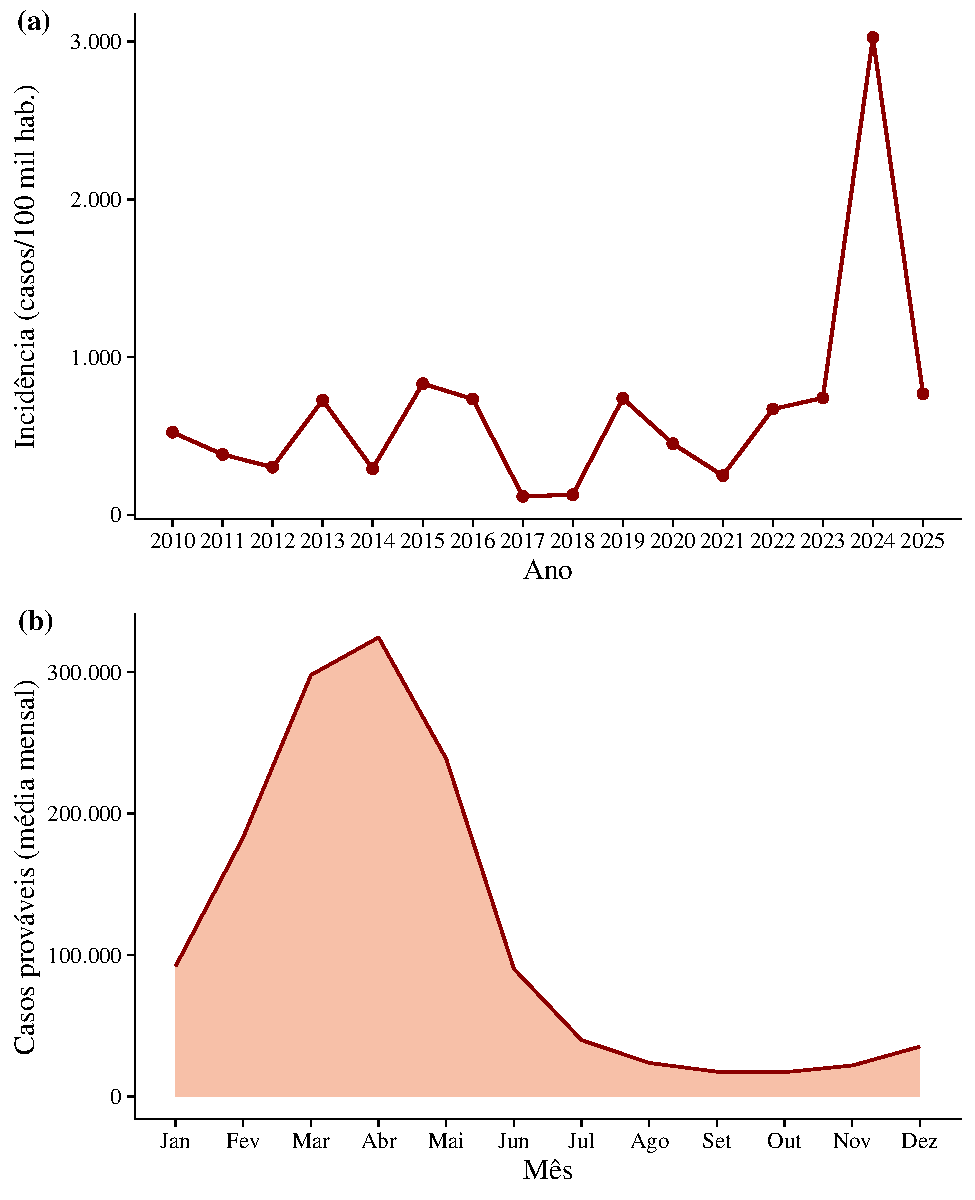
\includegraphics[width=0.95\textwidth]{fig_serie_temporal_dengue.pdf}
    \caption{Série temporal da dengue no Brasil, 2010--2025: (a) taxa de incidência anual, em casos prováveis por 100 mil habitantes; (b) média mensal de casos prováveis, em casos. Fontes: SINAN e IBGE.}
    \label{fig:serie_temporal}
\end{figure}

O padrão sazonal observado no painel (b) concentra a transmissão no primeiro semestre, com máximo em abril, seguido de março e de maio.

\subsection{Distribuição regional da incidência}

A Figura~\ref{fig:series_regioes} apresenta as séries temporais anuais da incidência por Grande Região, com a linha tracejada representando o valor nacional como referência. As regiões Centro-Oeste e Sudeste concentraram as maiores incidências acumuladas do período, com taxas de \TIRegiaoCentroOeste{} e \TIRegiaoSudeste{} casos por 100 mil habitantes, respectivamente, seguidas pelas regiões Sul (\TIRegiaoSul{}), Nordeste (\TIRegiaoNordeste{}) e Norte (\TIRegiaoNorte{}).

\begin{figure}[H]
    \centering
    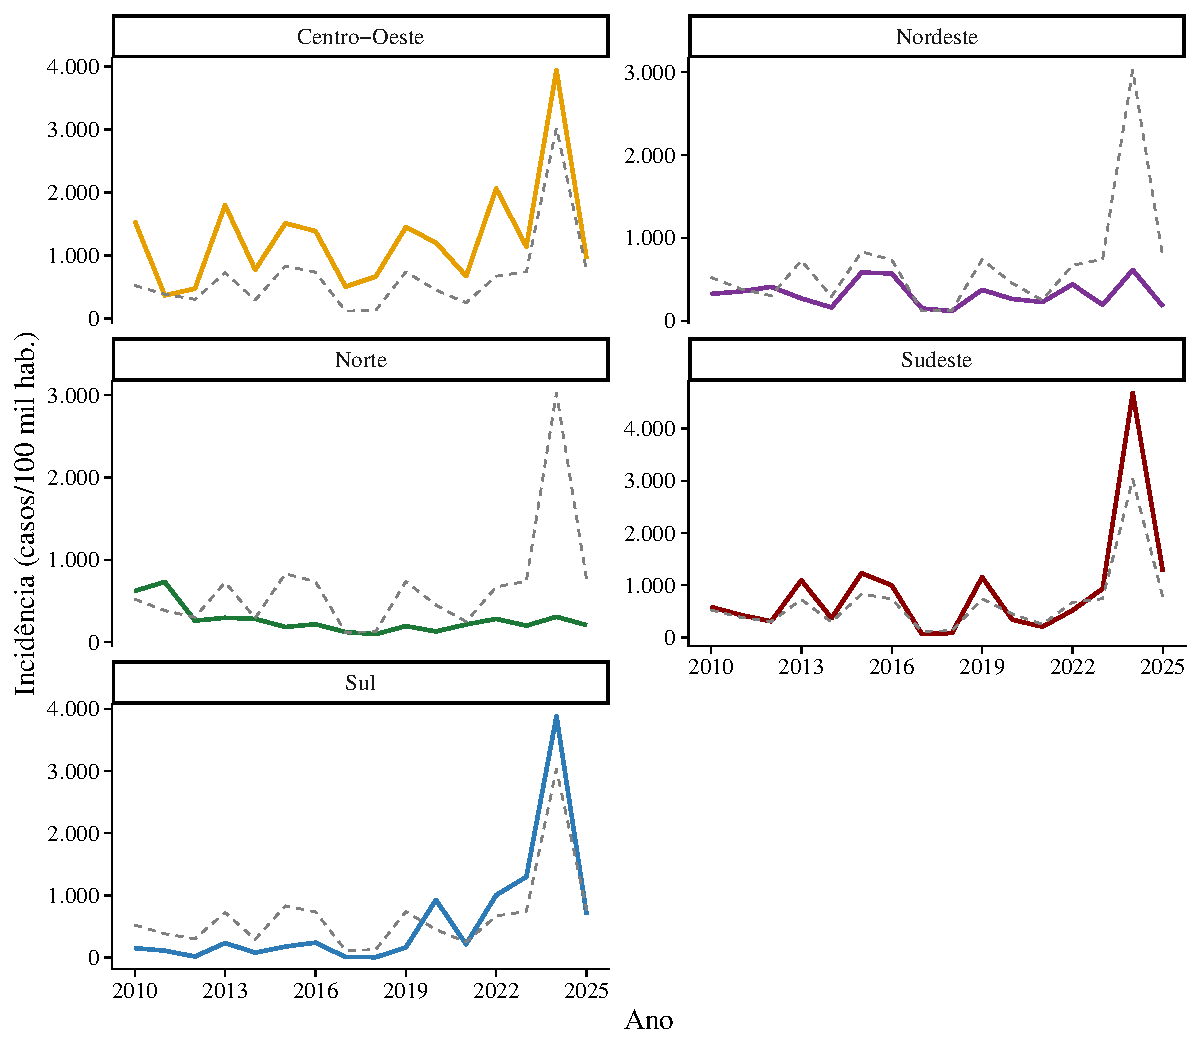
\includegraphics[width=0.95\textwidth]{fig_series_regioes.pdf}
    \caption{Taxa de incidência anual de dengue por Grande Região, Brasil, 2010--2025, em casos por 100 mil habitantes, com referência nacional tracejada. Fontes: SINAN e IBGE.}
    \label{fig:series_regioes}
\end{figure}

\begin{figure}[H]
    \centering
    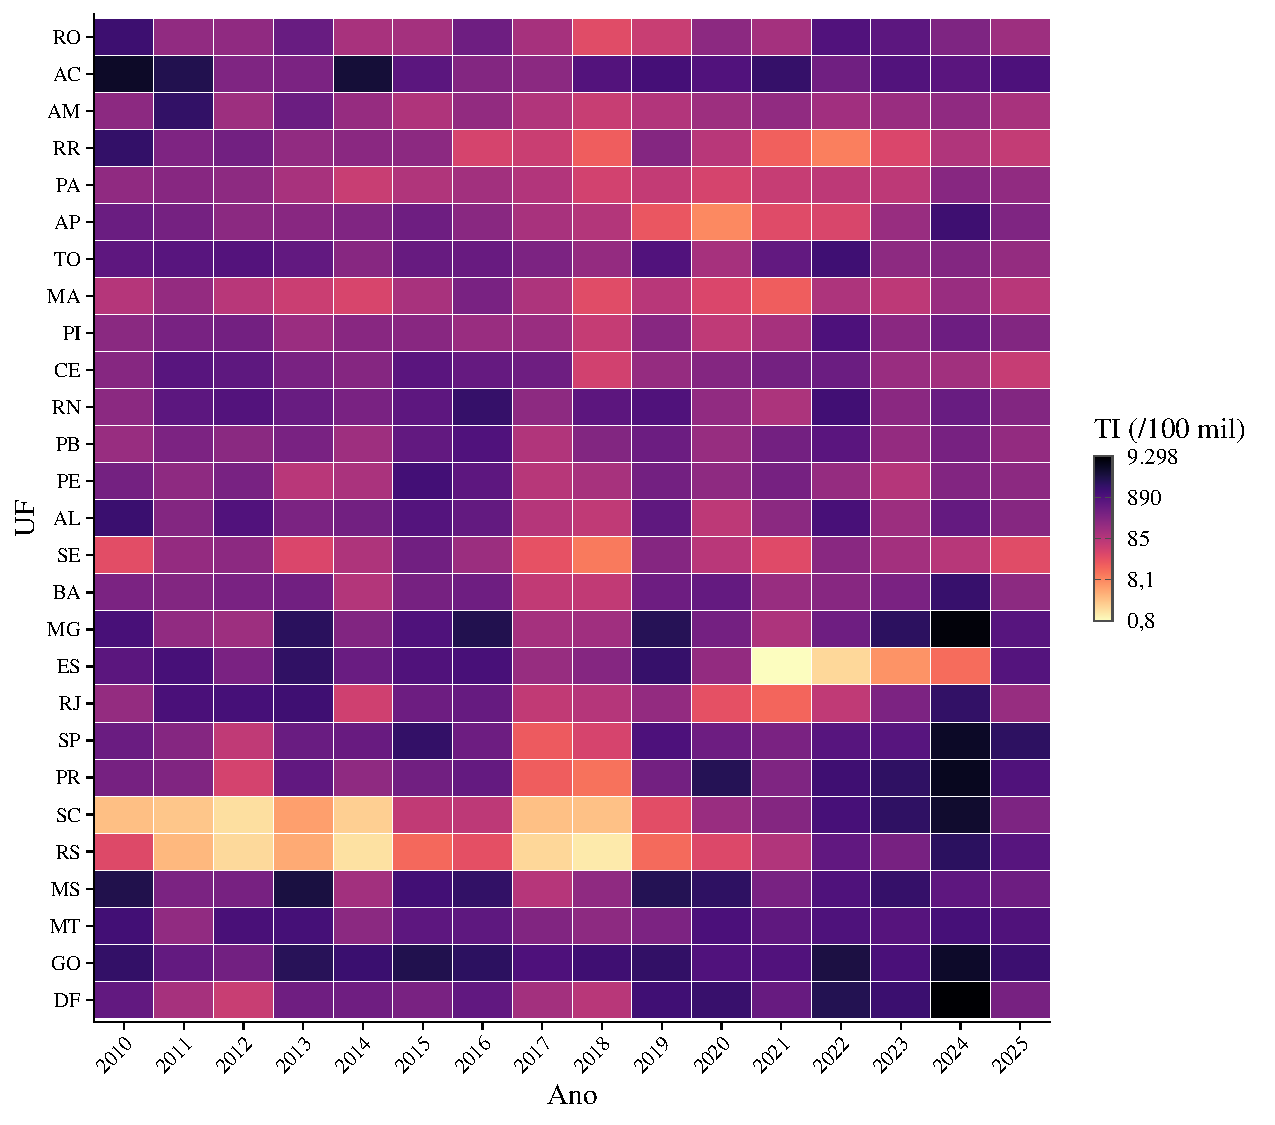
\includegraphics[width=0.95\textwidth]{fig_heatmap_incidencia_uf_ano.pdf}
    \caption{Taxa de incidência de dengue por UF e ano, Brasil, 2010--2025, em casos por 100 mil habitantes, com cor em logaritmo de base 10. Fontes: SINAN e IBGE.}
    \label{fig:heatmap_uf_ano}
    \vspace{0.3em}
    {\footnotesize\noindent\textit{Nota:} A taxa vai de \TIMinTI{} (\TIMinUF{} em \TIMinUFAno{}) a \TIMaxTI{} (\TIMaxUF{} em \TIMaxUFAno{}); em escala linear, os valores baixos comprimem a escala e reduzem o contraste.\par}
\end{figure}

A Figura~\ref{fig:heatmap_uf_ano} abre o mesmo dado por UF e ano. O ano de 2024 corresponde ao máximo de incidência em 10 das 27 UFs; em seguida vêm 2010, com 5 UFs, e 2011 e 2016, com 3 cada. Na Região Sul, as incidências anuais elevaram-se a partir da segunda metade do período 2010--2025.

\subsection{Autocorrelação espacial}

A Figura~\ref{fig:evolucao_moran} apresenta a evolução anual do Índice Global de Moran para a taxa de incidência municipal, calculado com matriz de vizinhança por contiguidade. O índice foi positivo e estatisticamente significativo em todos os anos do período (nível de 5\%), variando de \MoranMin{} a \MoranMax{}.

\begin{figure}[H]
    \centering
    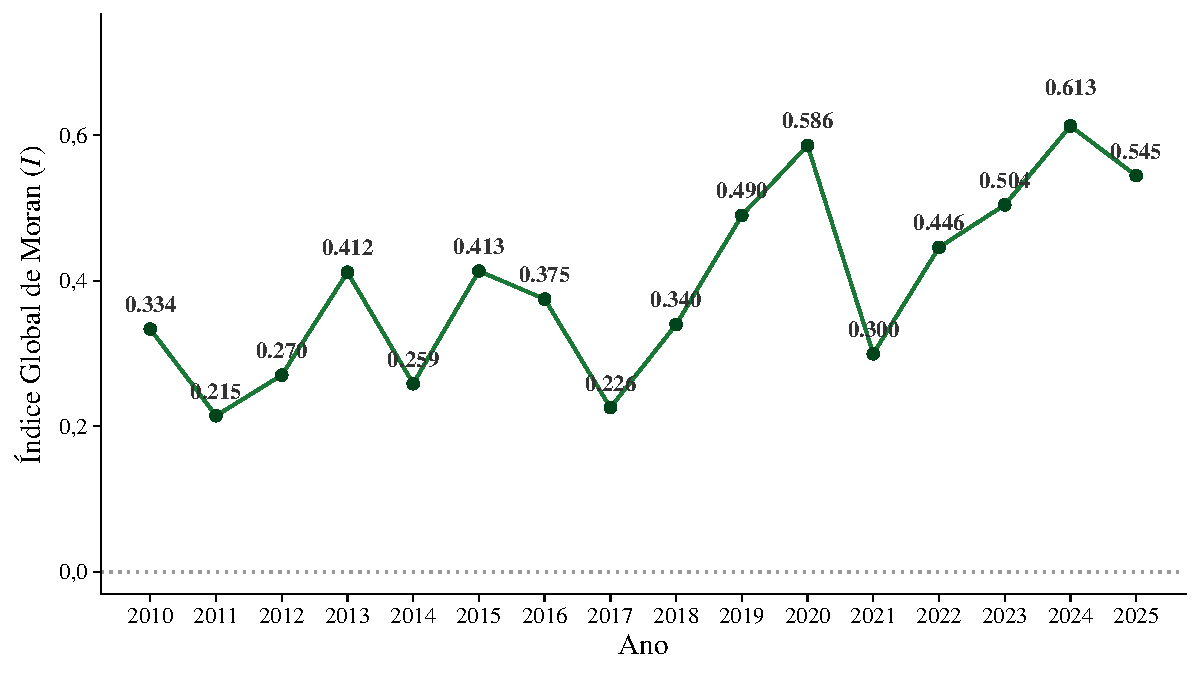
\includegraphics[width=0.95\textwidth]{fig_evolucao_moran.pdf}
    \caption{Evolução anual do Índice Global de Moran para a taxa de incidência municipal de dengue, Brasil, 2010--2025, calculado sobre casos prováveis por 100 mil habitantes. Fontes: SINAN e IBGE.}
    \label{fig:evolucao_moran}
\end{figure}

A autocorrelação espacial variou ao longo do tempo, com valores mais elevados nos anos de 2020 e, em especial, 2024 (\MoranDoisMilVinteQuatro{}), onde a incidência atingiu seu máximo. Valores relativamente menores foram encontrados nos anos 2011, 2017 e 2014.

Para identificar onde se concentram os \textit{clusters} de alto e de baixo risco, aplicou-se o Moran Local (LISA) à razão acumulada de casos por população média no período (2010--2025), com a mesma estrutura de vizinhança do índice global e 999 simulações condicionais (nível nominal de 5\%), sem correção para comparações múltiplas. A Figura~\ref{fig:mapa_lisa} apresenta a classificação dos municípios nos quadrantes do diagrama de dispersão de Moran: \LisaSig{} municípios (\LisaPctSig{}) foram classificados como associação local significativa pelo valor-p bilateral por simulação, dos quais \LisaHH{} (\LisaPctHH{}) formam o quadrante alto-alto e \LisaLL{} (\LisaPctLL{}) o quadrante baixo-baixo; os quadrantes alto-baixo e baixo-alto reuniram apenas \LisaHL{} e \LisaLH{} municípios, respectivamente, enquanto os \LisaNS{} municípios restantes (\LisaPctNS{}) não atingiram o nível nominal de significância.

\begin{figure}[H]
    \centering
    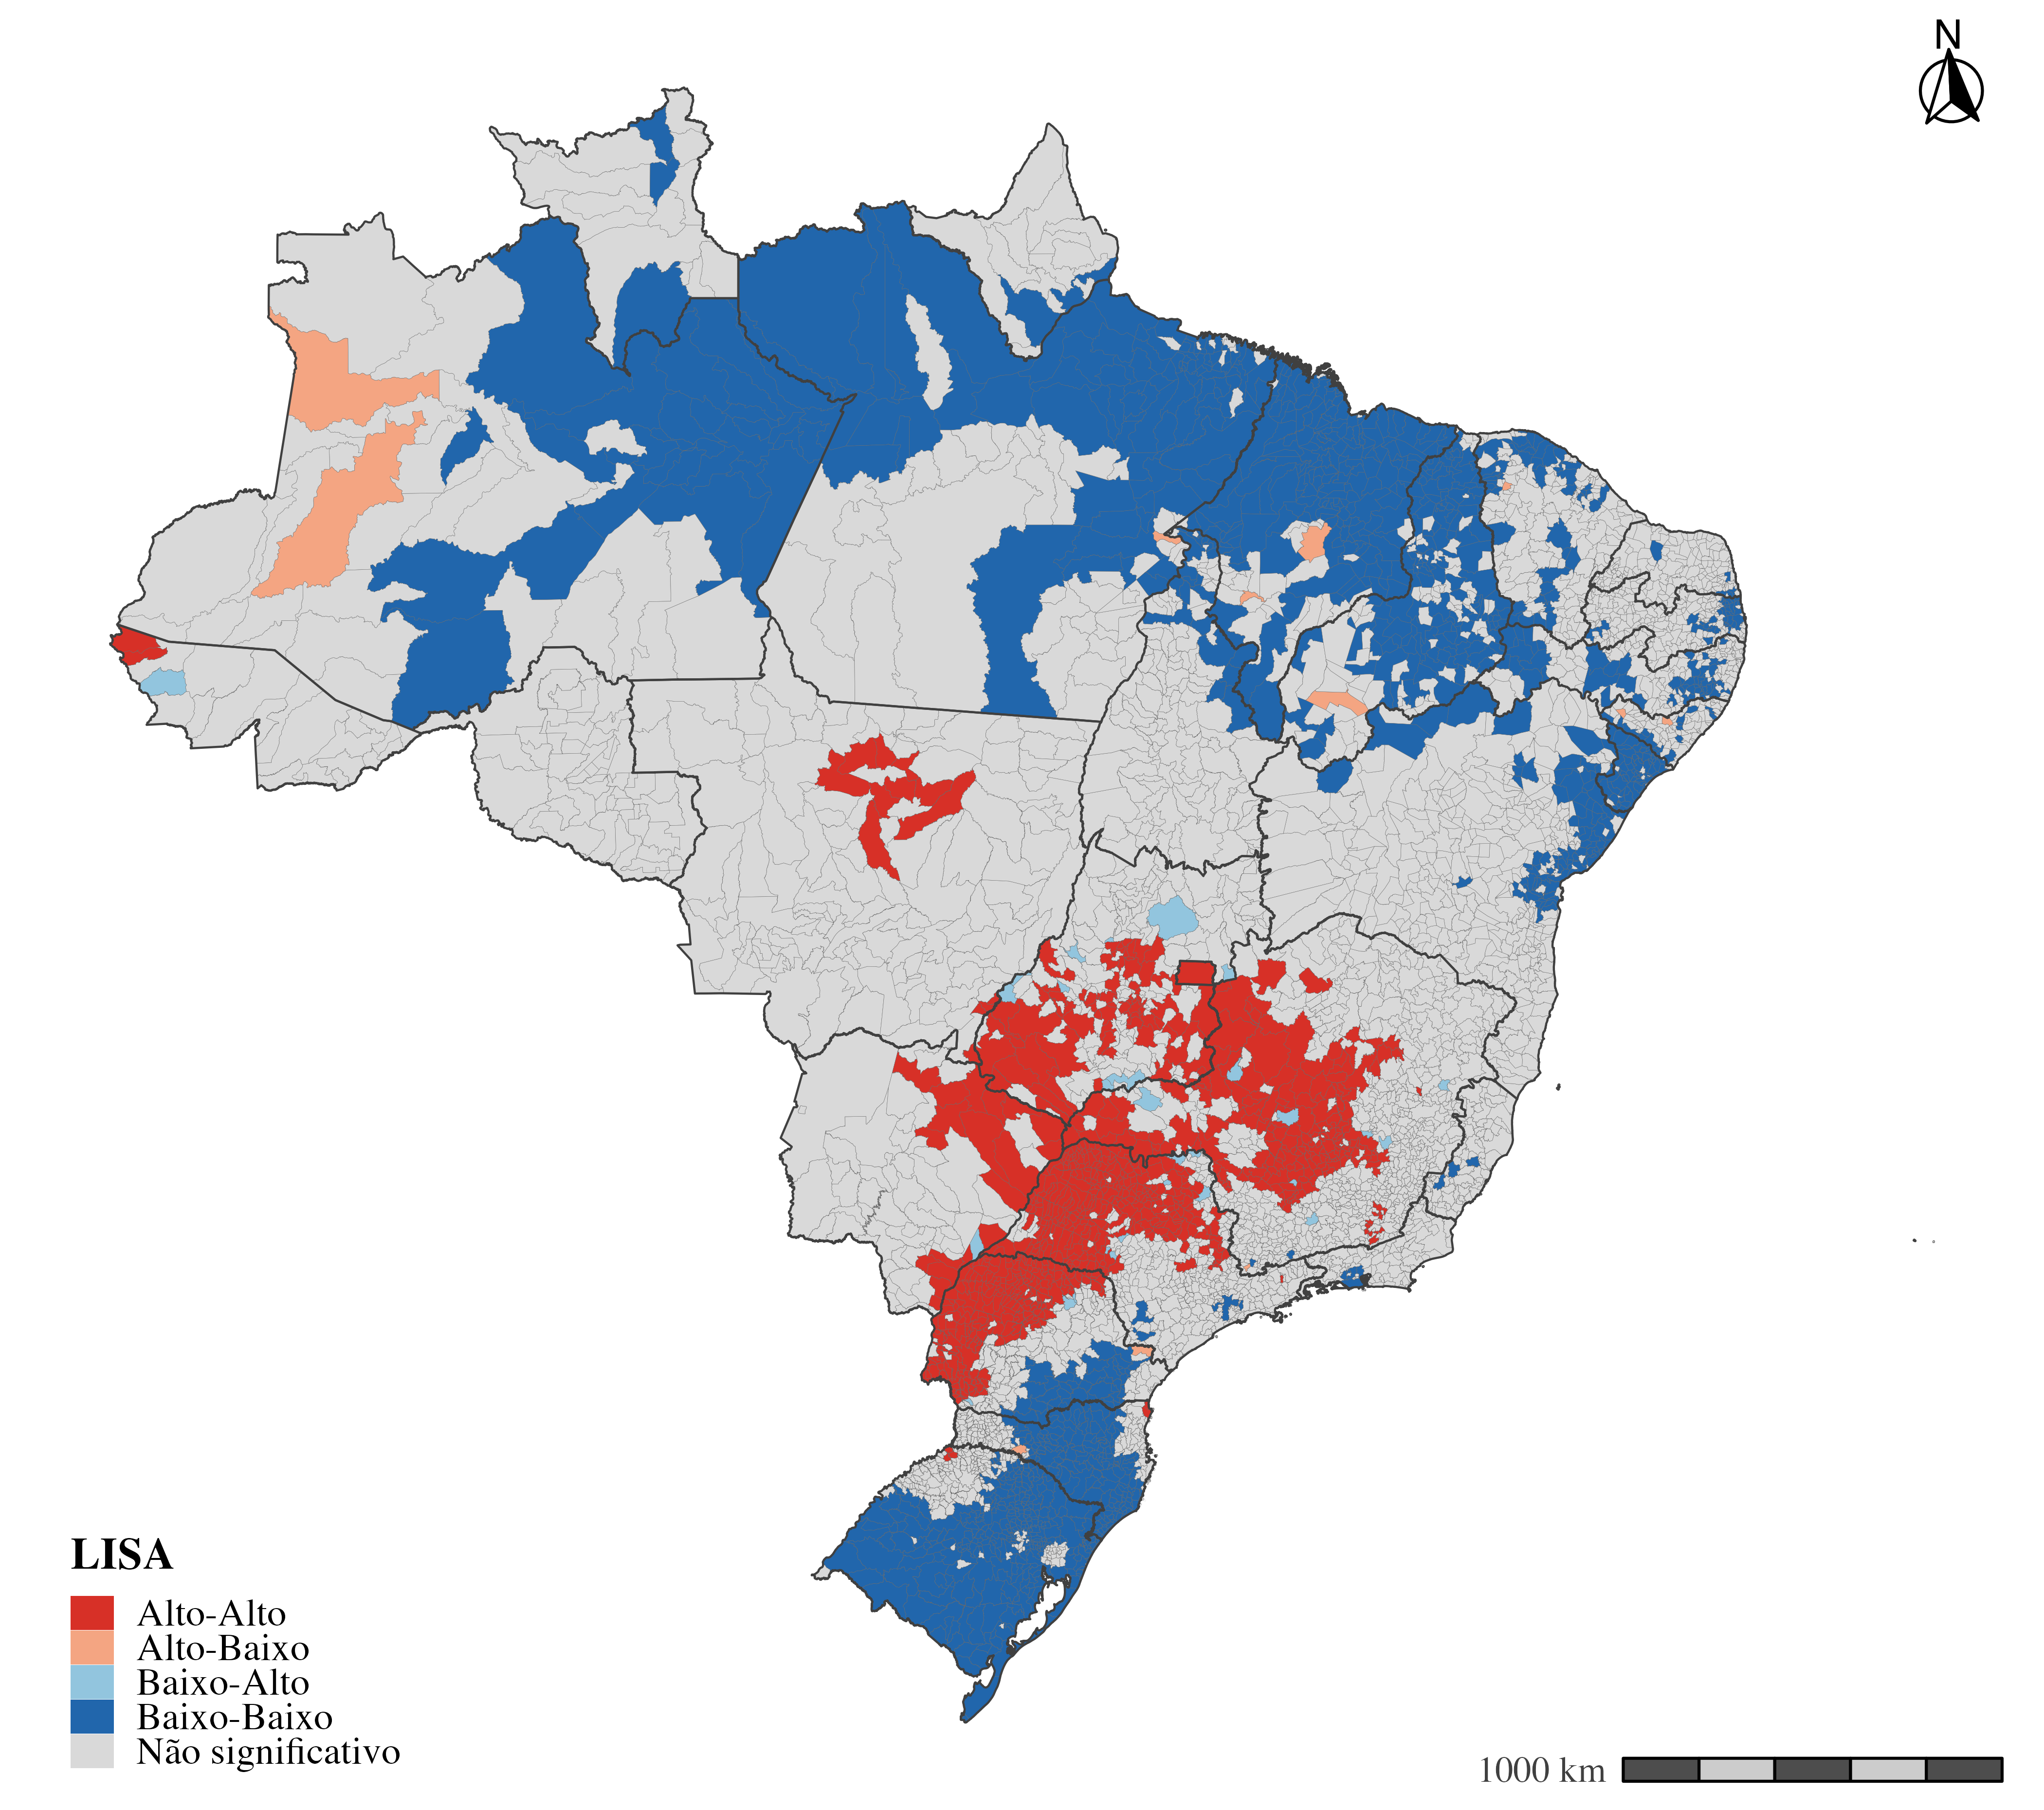
\includegraphics[width=0.64\textwidth]{fig_mapa_lisa.png}
    \caption{Quadrantes locais de associação espacial da razão acumulada de casos por população média, Brasil, 2010--2025. Fontes: SINAN e IBGE.}
    \label{fig:mapa_lisa}
    \vspace{0.3em}
    {\footnotesize\noindent\textit{Nota:} Classificação local com 999 simulações condicionais e nível nominal de 5\%.\par}
\end{figure}

\subsection{Caracterização socioespacial e climática}

As Tabelas~\ref{tab:resumo_socioespacial} e \ref{tab:resumo_clima} sintetizam, por Grande Região e para o Brasil, as medidas-resumo das variáveis socioespaciais (Censo 2022) e climáticas (reanálise climática), respectivamente.

\begin{table}[!h]
\centering
\caption{\label{tab:resumo_socioespacial}Medidas-resumo das variáveis socioespaciais por Grande Região (Censo 2022).}
\centering
\resizebox{\ifdim\width>\linewidth\linewidth\else\width\fi}{!}{
\fontsize{9}{11}\selectfont
\begin{tabular}[t]{lcccccc}
\toprule
Medida & Brasil & Norte & Nordeste & Sudeste & Sul & Centro-Oeste\\
\midrule
\addlinespace[0.3em]
\multicolumn{7}{l}{\textbf{Abastecimento de água por rede geral (\%)}}\\
\hspace{1em}Média (D.P.) & 71,7 (19,6) & 53,4 (22,8) & 67,3 (20,0) & 79,1 (15,6) & 74,3 (18,1) & 73,5 (15,4)\\
\hspace{1em}Mediana (IIQ) & 75,8 (26,2) & 57,6 (32,9) & 70,5 (25,4) & 82,8 (21,7) & 78,7 (25,8) & 75,7 (17,8)\\
\hspace{1em}Mínimo–Máximo & 0,0 – 100,0 & 0,0 – 95,0 & 0,0 – 99,6 & 22,5 – 100,0 & 10,2 – 99,6 & 3,4 – 96,6\\
\addlinespace[0.3em]
\multicolumn{7}{l}{\textbf{Esgotamento sanitário por rede (\%)}}\\
\hspace{1em}Média (D.P.) & 37,7 (33,0) & 7,4 (12,4) & 24,4 (23,9) & 70,6 (23,4) & 29,8 (29,3) & 20,7 (25,4)\\
\hspace{1em}Mediana (IIQ) & 32,3 (63,7) & 2,5 (6,4) & 17,0 (38,1) & 76,8 (32,3) & 18,9 (51,3) & 6,6 (34,0)\\
\hspace{1em}Mínimo–Máximo & 0,0 – 99,9 & 0,0 – 76,6 & 0,0 – 95,1 & 0,1 – 99,9 & 0,0 – 98,1 & 0,0 – 94,3\\
\addlinespace[0.3em]
\multicolumn{7}{l}{\textbf{Coleta de lixo (\%)}}\\
\hspace{1em}Média (D.P.) & 80,2 (17,4) & 66,2 (17,0) & 70,7 (17,8) & 89,1 (12,5) & 86,8 (13,5) & 81,6 (13,0)\\
\hspace{1em}Mediana (IIQ) & 85,1 (25,5) & 66,7 (25,8) & 72,5 (25,1) & 94,2 (12,3) & 91,3 (16,4) & 84,6 (17,1)\\
\hspace{1em}Mínimo–Máximo & 1,7 – 100,0 & 13,6 – 98,8 & 1,7 – 99,6 & 24,1 – 100,0 & 31,3 – 100,0 & 29,1 – 99,8\\
\addlinespace[0.3em]
\multicolumn{7}{l}{\textbf{População em favelas (\%)}}\\
\hspace{1em}Média (D.P.) & 1,0 (4,3) & 3,1 (8,9) & 0,8 (3,9) & 1,2 (4,2) & 0,5 (2,5) & 0,2 (1,1)\\
\hspace{1em}Mediana (IIQ) & 0,0 (0,0) & 0,0 (0,0) & 0,0 (0,0) & 0,0 (0,0) & 0,0 (0,0) & 0,0 (0,0)\\
\hspace{1em}Mínimo–Máximo & 0,0 – 69,2 & 0,0 – 69,2 & 0,0 – 45,4 & 0,0 – 42,6 & 0,0 – 47,2 & 0,0 – 11,8\\
\addlinespace[0.3em]
\multicolumn{7}{l}{\textbf{Densidade demográfica (hab/km²)}}\\
\hspace{1em}Média (D.P.) & 113,8 (585,8) & 23,1 (142,2) & 89,1 (395,6) & 205,7 (942,0) & 87,0 (285,8) & 36,1 (207,1)\\
\hspace{1em}Mediana (IIQ) & 24,1 (41,8) & 4,1 (9,0) & 28,6 (48,5) & 30,8 (53,0) & 25,5 (33,9) & 5,8 (12,2)\\
\hspace{1em}Mínimo–Máximo & 0,2 – 13.328,0 & 0,2 – 2.501,1 & 1,0 – 7.958,5 & 1,2 – 13.328,0 & 1,5 – 4.065,9 & 0,3 – 3.221,8\\
\bottomrule
\end{tabular}}
\end{table}


\begin{table}[!h]
\centering
\caption{\label{tab:resumo_clima}Medidas-resumo das variáveis climáticas por Grande Região, Brasil, 2010--2025.}
\centering
\resizebox{\ifdim\width>\linewidth\linewidth\else\width\fi}{!}{
\fontsize{9}{11}\selectfont
\begin{tabular}[t]{lcccccc}
\toprule
Medida & Brasil & Norte & Nordeste & Sudeste & Sul & Centro-Oeste\\
\midrule
\addlinespace[0.3em]
\multicolumn{7}{l}{\textbf{Temperatura máxima extrema anual (°C)}}\\
\hspace{1em}Média (D.P.) & 35,2 (2,5) & 36,2 (1,8) & 35,4 (2,4) & 34,9 (2,6) & 33,9 (2,4) & 37,4 (1,6)\\
\hspace{1em}Mediana (IIQ) & 35,4 (3,8) & 36,4 (2,3) & 35,8 (3,7) & 35,0 (3,6) & 34,0 (3,5) & 37,4 (2,2)\\
\hspace{1em}Mínimo–Máximo & 25,6 – 42,7 & 30,0 – 40,9 & 28,6 – 40,6 & 25,6 – 42,7 & 25,8 – 41,2 & 32,2 – 42,3\\
\addlinespace[0.3em]
\multicolumn{7}{l}{\textbf{Dias sob onda de calor (dias/ano)}}\\
\hspace{1em}Média (D.P.) & 24,1 (16,3) & 27,2 (21,3) & 22,7 (15,7) & 24,1 (16,7) & 22,8 (14,0) & 29,8 (15,5)\\
\hspace{1em}Mediana (IIQ) & 22,0 (22,0) & 24,0 (26,0) & 21,0 (21,0) & 22,0 (22,0) & 21,0 (21,0) & 29,0 (22,0)\\
\hspace{1em}Mínimo–Máximo & 0,0 – 151,0 & 0,0 – 151,0 & 0,0 – 100,0 & 0,0 – 104,0 & 0,0 – 83,0 & 0,0 – 86,0\\
\addlinespace[0.3em]
\multicolumn{7}{l}{\textbf{Umidade relativa média (\%)}}\\
\hspace{1em}Média (D.P.) & 70,7 (7,8) & 75,2 (8,2) & 69,3 (8,7) & 69,3 (6,6) & 75,5 (5,0) & 64,3 (5,0)\\
\hspace{1em}Mediana (IIQ) & 71,7 (12,1) & 77,5 (12,9) & 71,0 (14,9) & 69,4 (9,5) & 75,6 (6,3) & 62,9 (6,9)\\
\hspace{1em}Mínimo–Máximo & 46,3 – 90,6 & 53,3 – 90,6 & 46,3 – 86,1 & 46,8 – 87,4 & 59,0 – 87,1 & 53,3 – 83,0\\
\addlinespace[0.3em]
\multicolumn{7}{l}{\textbf{Precipitação anual acumulada (mm)}}\\
\hspace{1em}Média (D.P.) & 1.262,1 (572,7) & 1.916,6 (623,3) & 881,4 (491,3) & 1.162,2 (373,6) & 1.682,9 (438,9) & 1.380,3 (388,4)\\
\hspace{1em}Mediana (IIQ) & 1.236,3 (742,4) & 1.833,6 (808,9) & 777,5 (640,4) & 1.158,1 (470,6) & 1.650,0 (579,5) & 1.344,8 (441,8)\\
\hspace{1em}Mínimo–Máximo & 0,2 – 7.139,7 & 15,0 – 5.472,4 & 0,2 – 5.411,0 & 0,2 – 6.775,8 & 17,8 – 4.886,0 & 90,8 – 7.139,7\\
\bottomrule
\end{tabular}}
\end{table}


Em nível nacional, a cobertura média municipal de abastecimento de água por rede geral foi de \MediaMunAgua{} (atingindo \PropAguaRedeBrasil{} quando ponderada pelo número de domicílios do município), de esgotamento sanitário por rede de \MediaMunEsgoto{} (\PropEsgotoRedeBrasil{} ponderada) e de coleta de resíduos sólidos de \MediaMunLixo{} (\PropLixoBrasil{} ponderada), enquanto a proporção média de população residente em favelas e comunidades urbanas nos municípios foi de \MediaMunFavela{} (\PropFavelaBrasil{} no agregado populacional nacional). A Região Norte apresentou os menores patamares de infraestrutura de saneamento, enquanto o Sudeste concentrou os maiores indicadores de cobertura, como detalhado na Tabela~\ref{tab:resumo_socioespacial}.

Quanto ao clima, a temperatura máxima extrema anual média municipal foi de 35,2~$^\circ$C (34,6~$^\circ$C quando ponderada pela população), com umidade relativa de 70,7\% (73,6\% ponderada) e precipitação anual de 1.262,1 mm (\PrecipAnualBrasil{} ponderada). As Figuras~\ref{fig:mapa_temperatura}, \ref{fig:mapa_precipitacao} e \ref{fig:mapa_umidade} mostram a heterogeneidade climática do território: as maiores temperaturas ocorreram no Centro-Oeste; as maiores médias municipais de umidade relativa, no Sul e no Norte; a maior pluviosidade, na Amazônia e no Sul; e a menor umidade relativa, no interior do Nordeste e do Centro-Oeste. O Sul apresentou as temperaturas mais amenas.

\begin{figure}[H]
    \centering
    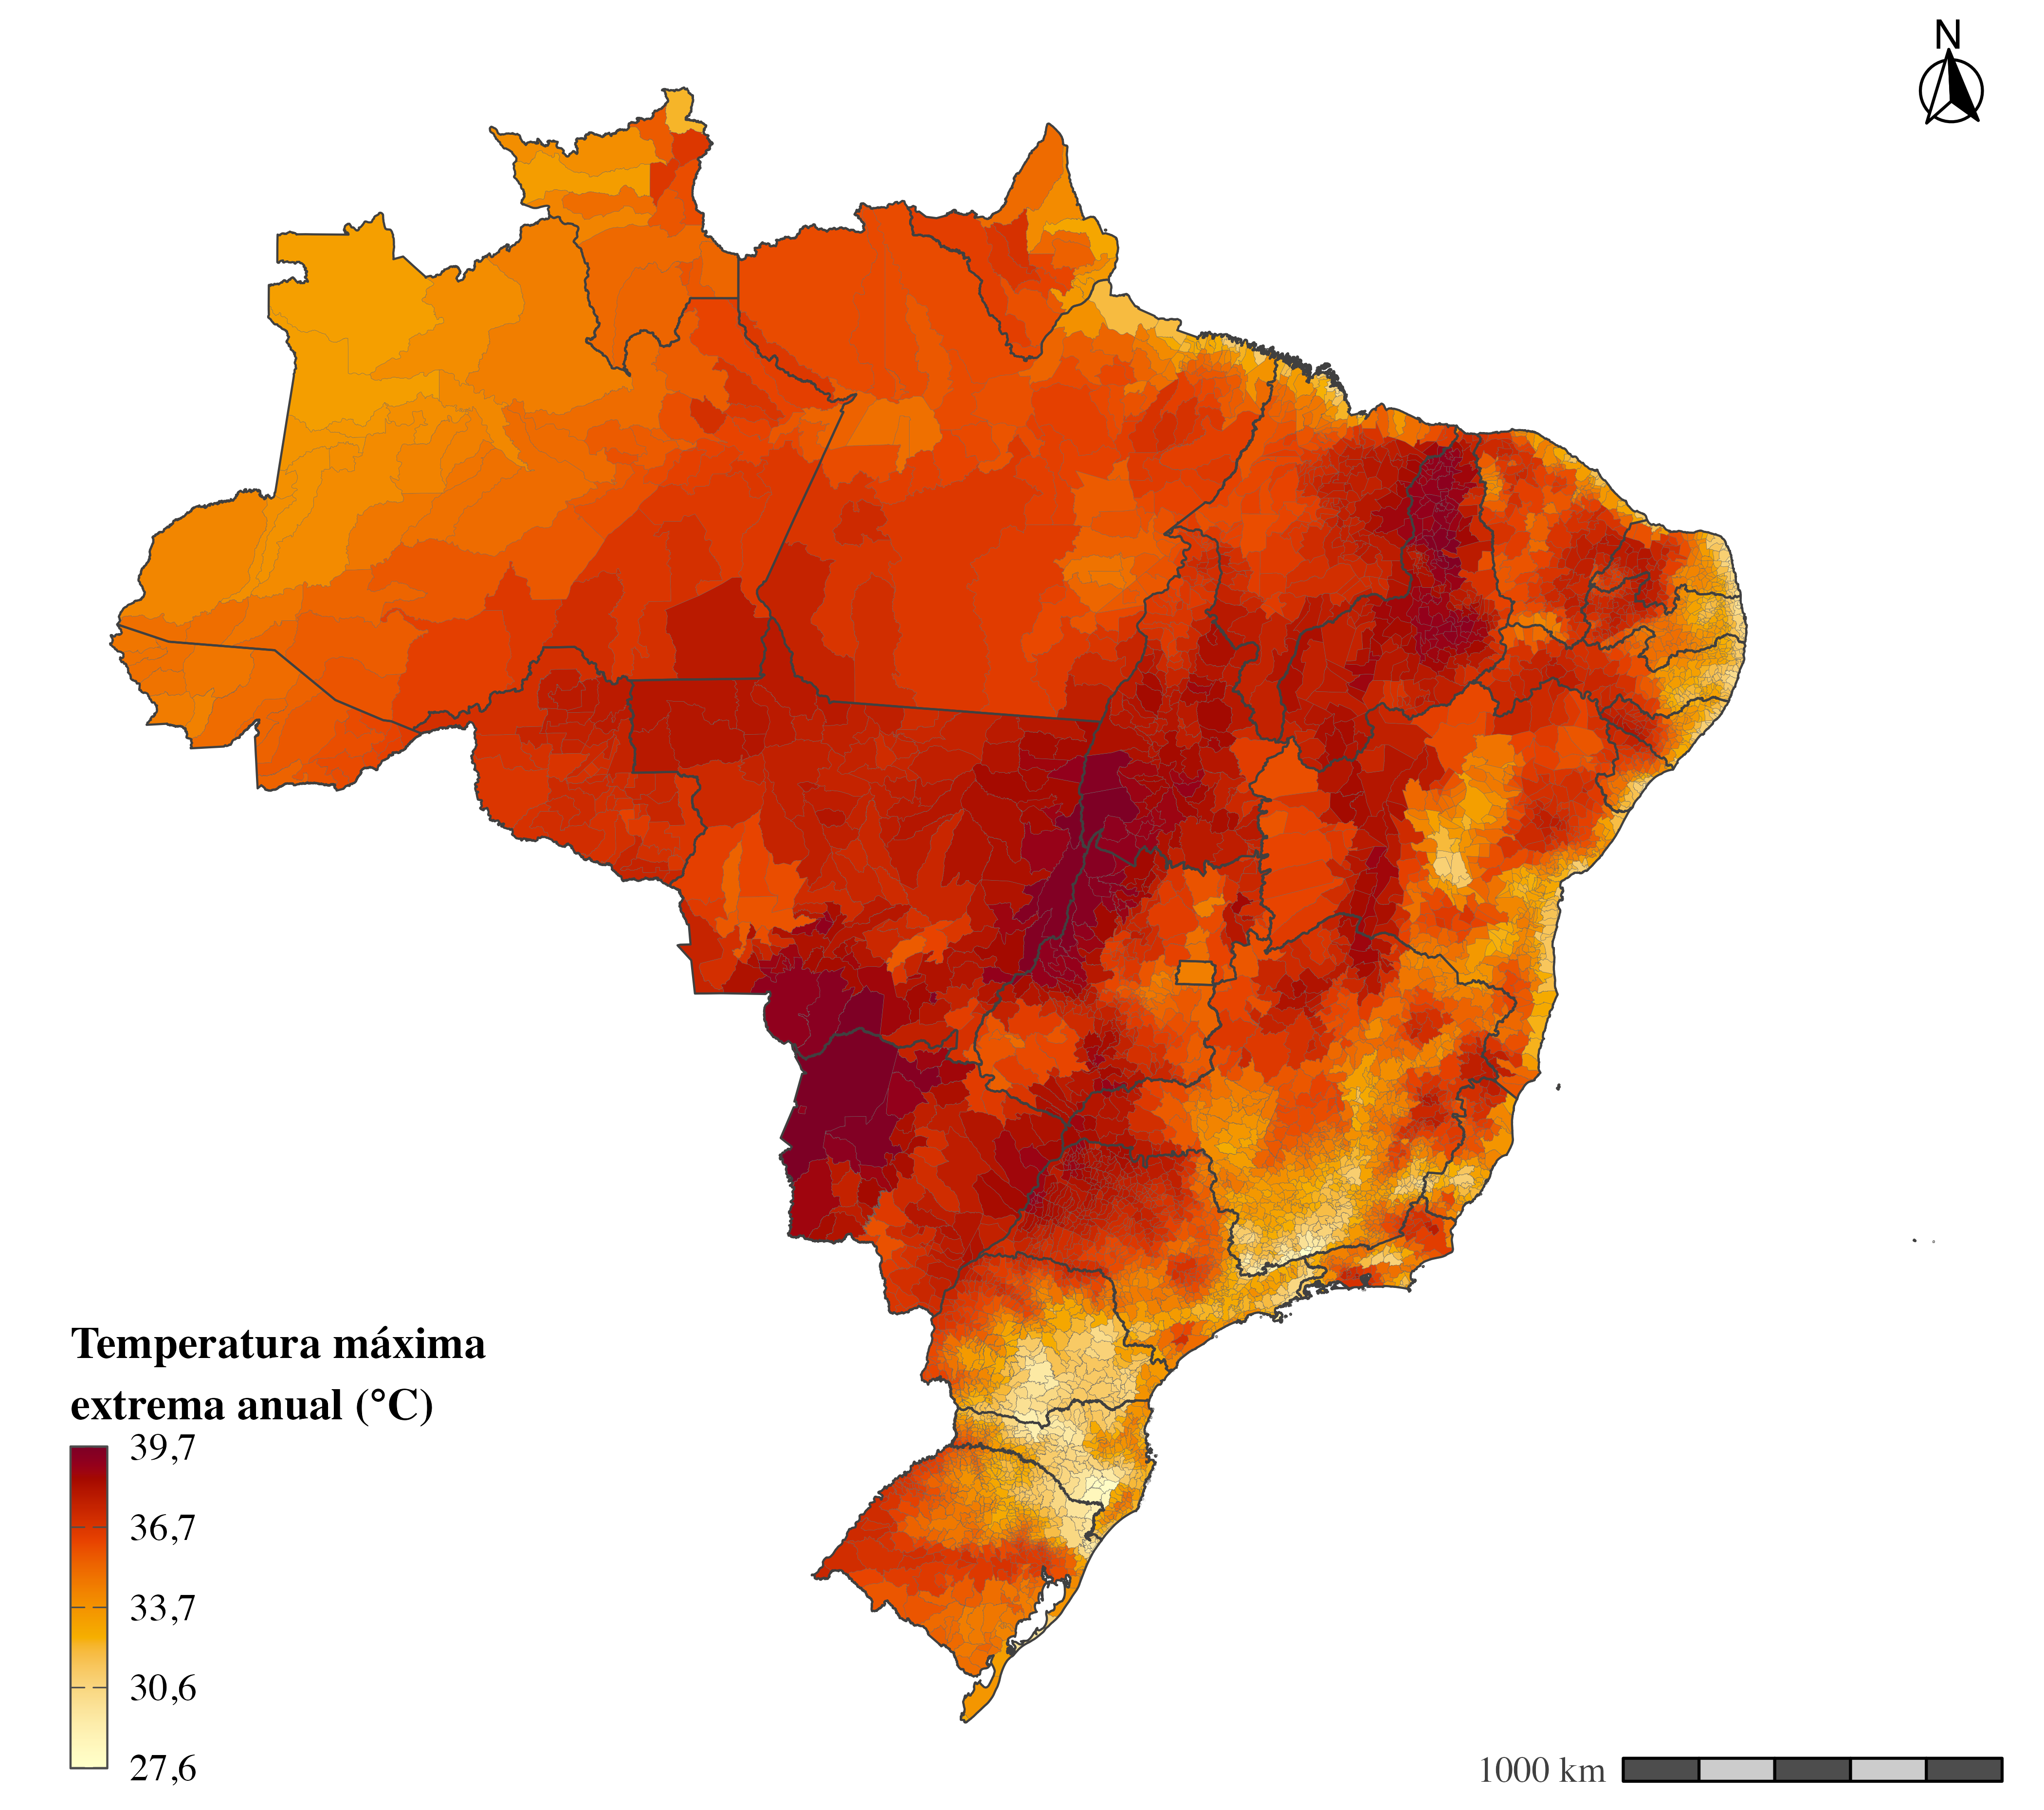
\includegraphics[width=0.64\textwidth]{fig_mapa_temperatura.png}
    \caption{Média municipal da máxima diária anual de temperatura, Brasil, 2010--2025, em graus Celsius. Fonte: reanálise climática.}
    \label{fig:mapa_temperatura}
\end{figure}

\begin{figure}[H]
    \centering
    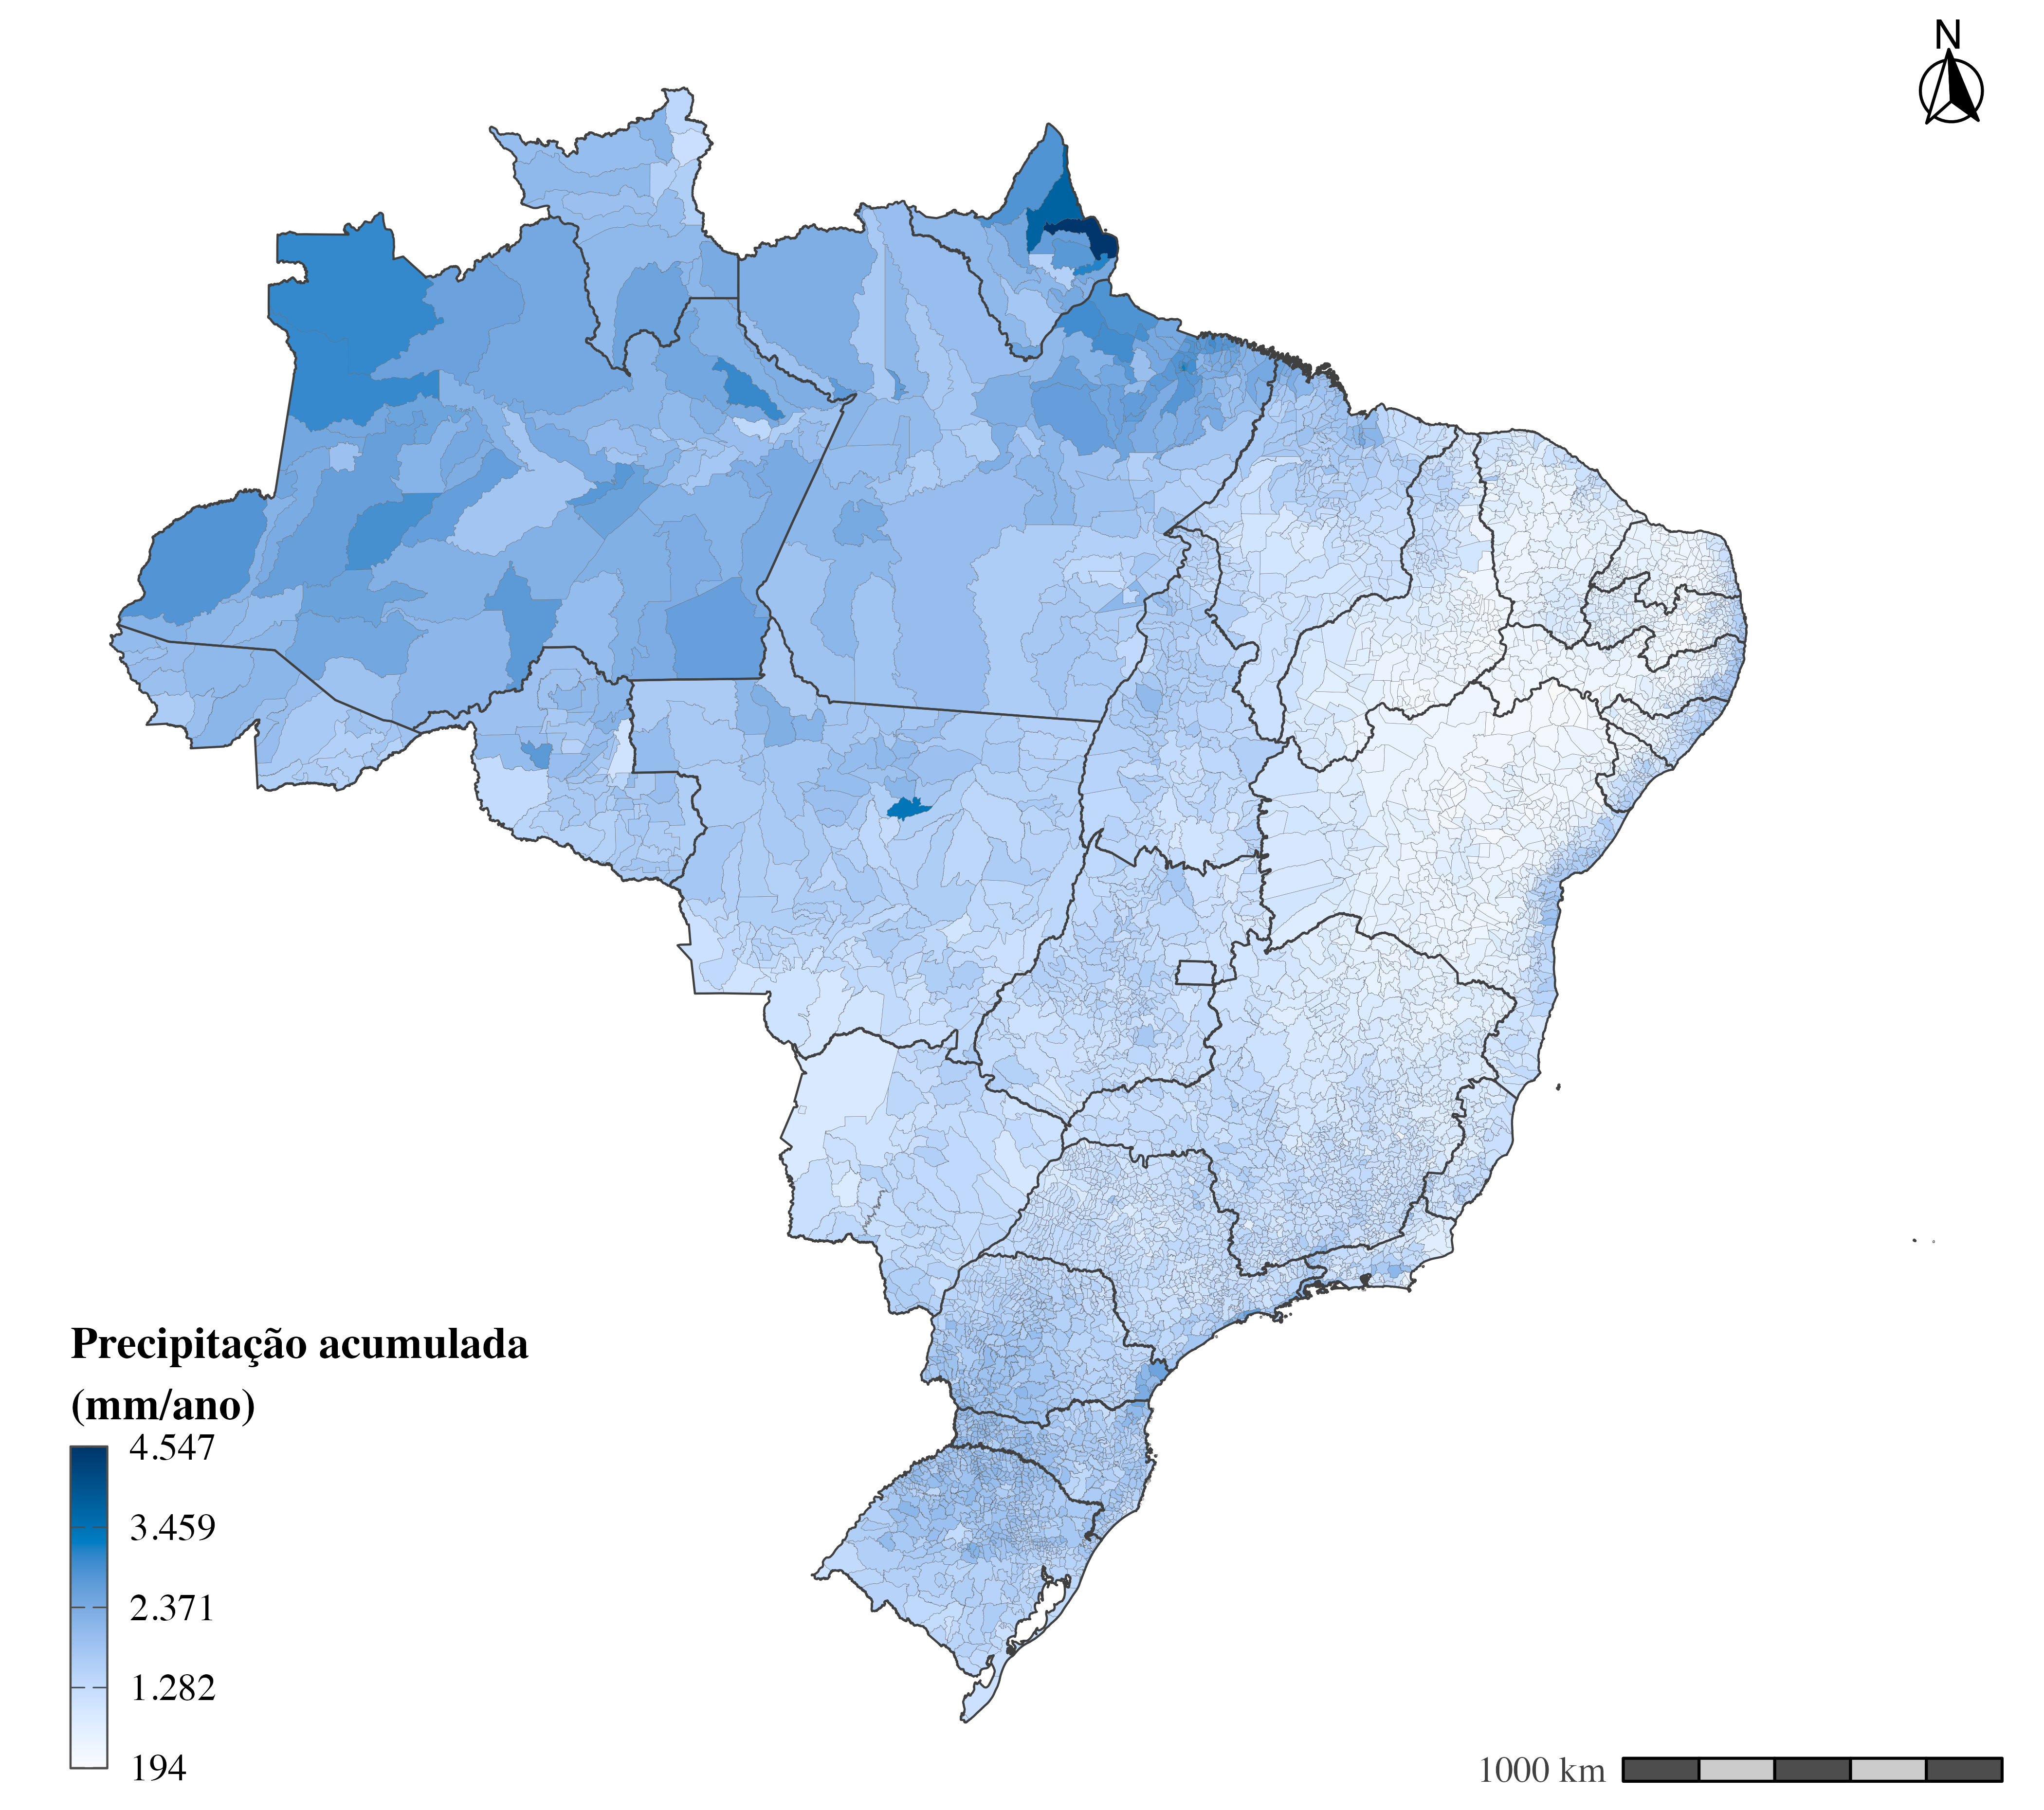
\includegraphics[width=0.64\textwidth]{fig_mapa_precipitacao.png}
    \caption{Precipitação anual acumulada por município, Brasil, 2010--2025, em milímetros por ano. Fonte: estações de superfície.}
    \label{fig:mapa_precipitacao}
\end{figure}

\begin{figure}[H]
    \centering
    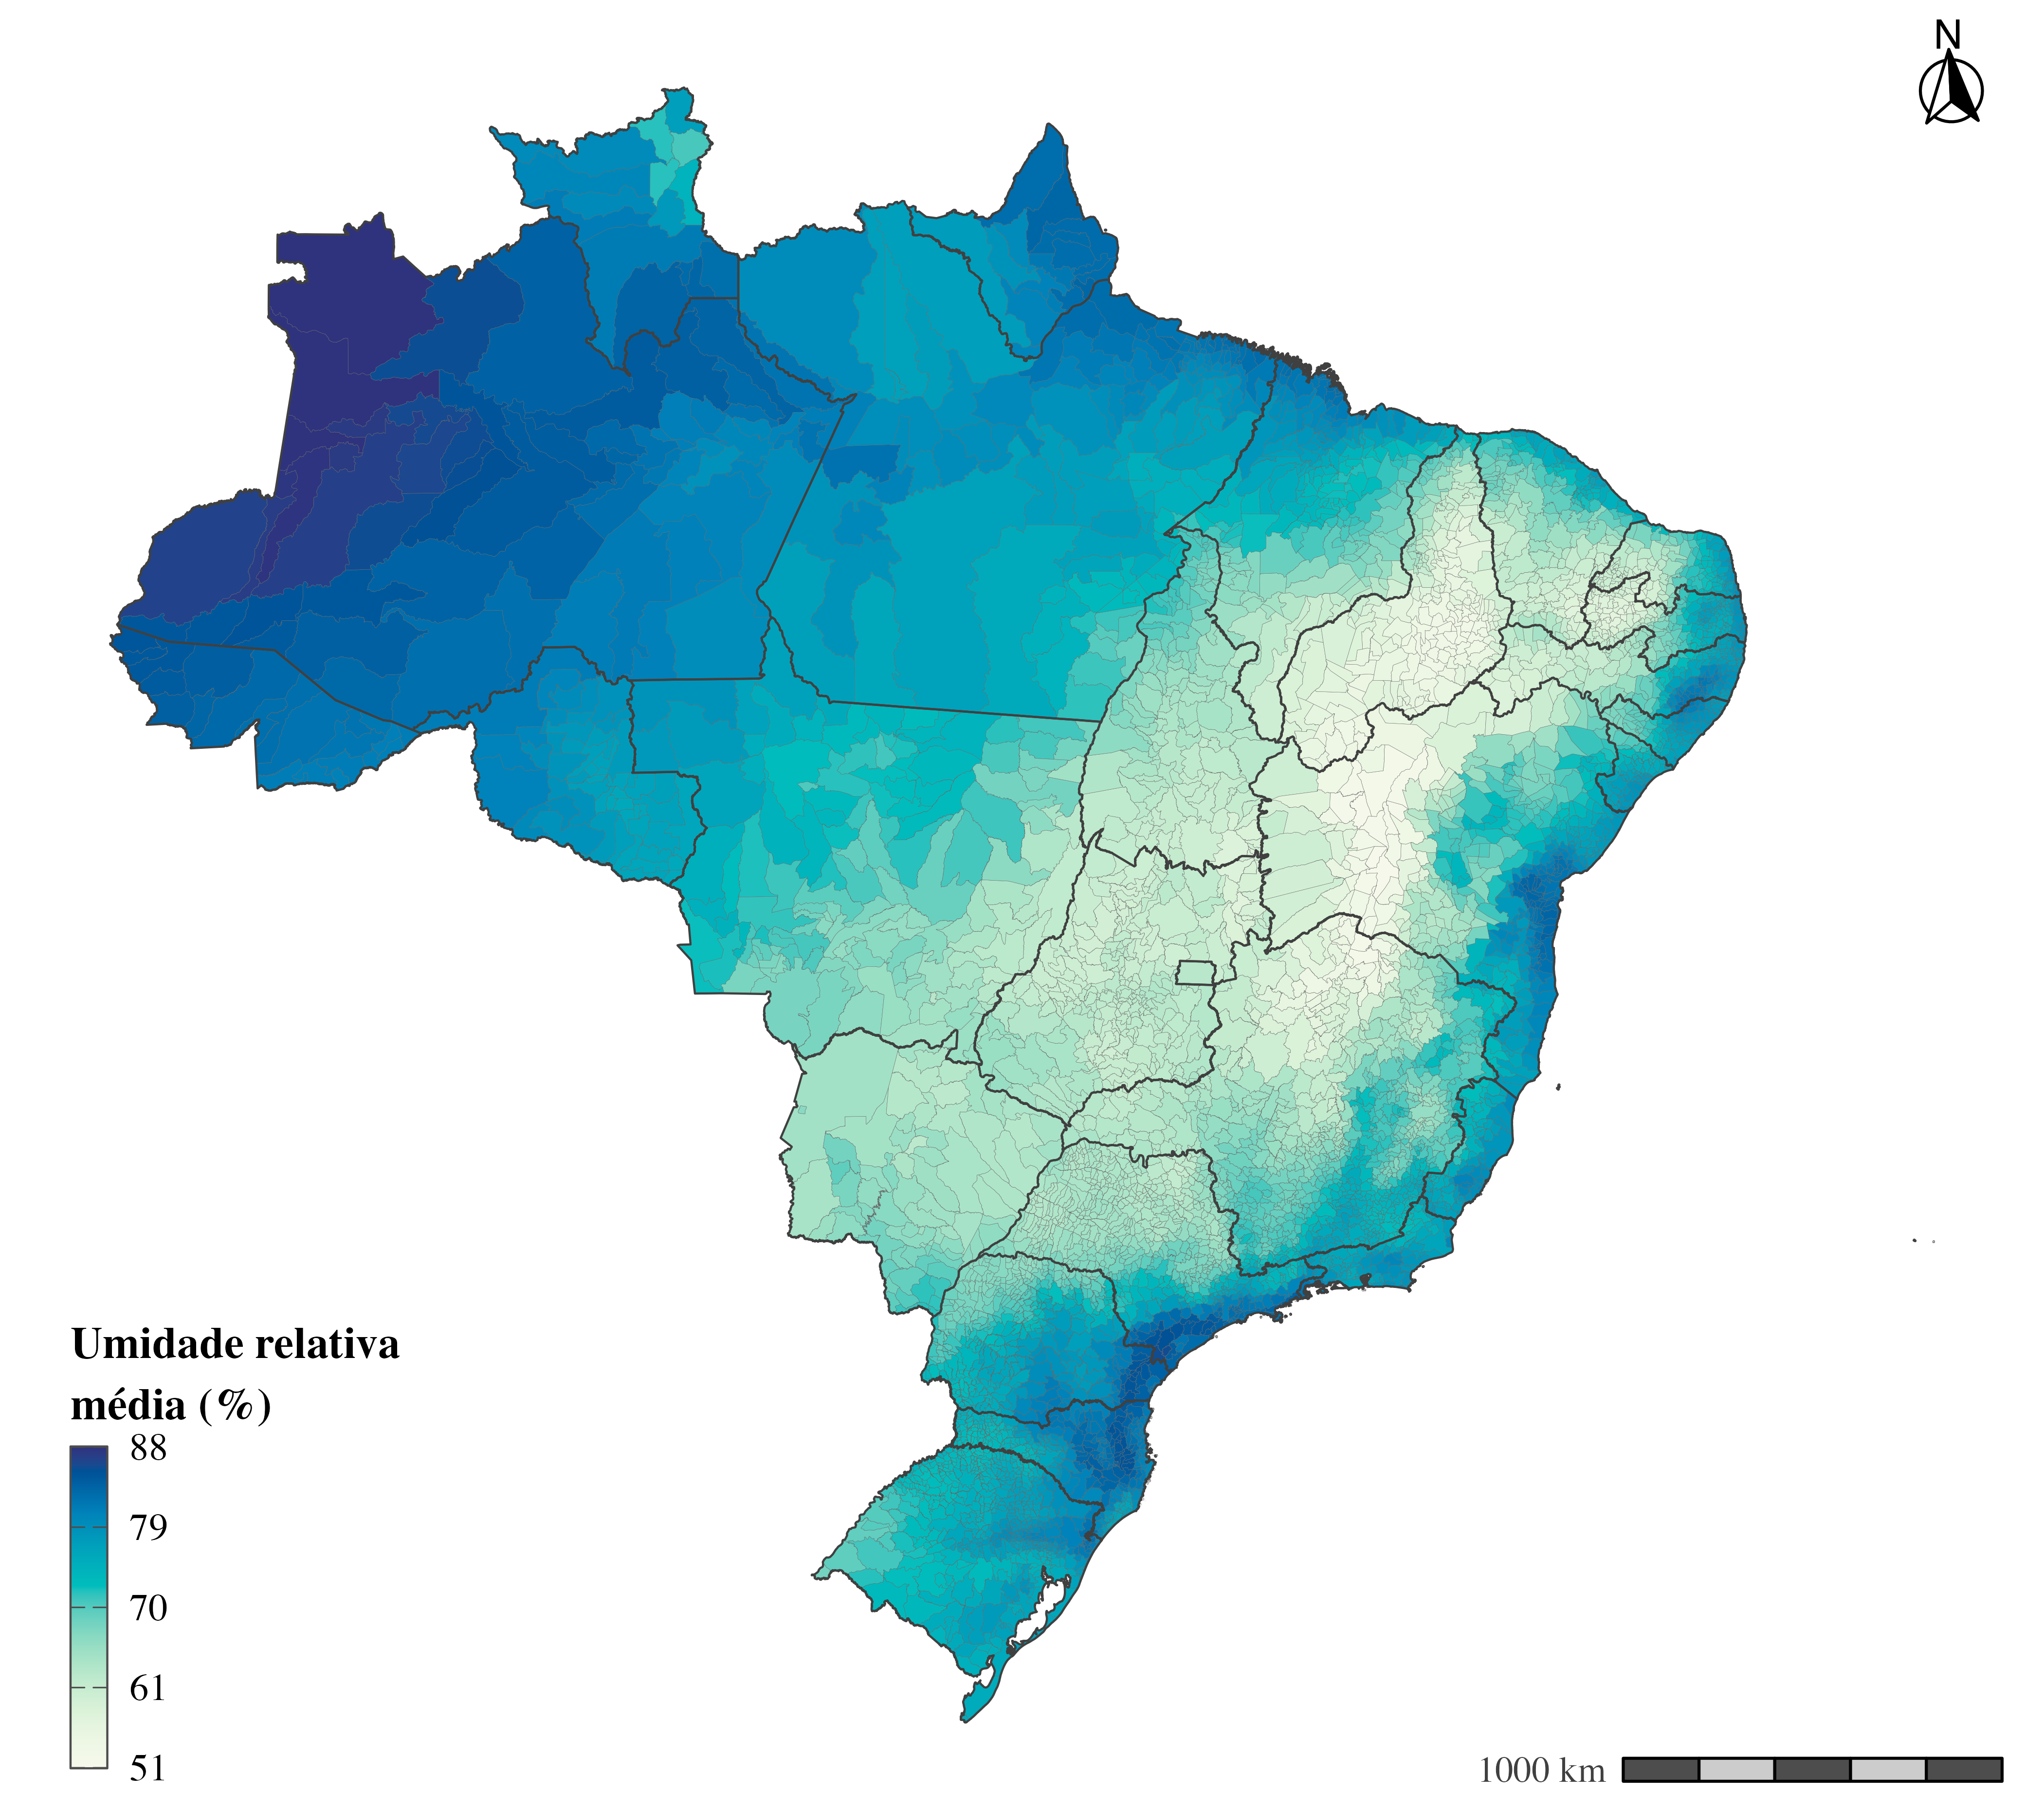
\includegraphics[width=0.64\textwidth]{fig_mapa_umidade.png}
    \caption{Média municipal da umidade relativa do ar, Brasil, 2010--2025, em percentual. Fonte: reanálise climática.}
    \label{fig:mapa_umidade}
\end{figure}

A variação mensal da temperatura acompanha o padrão descrito na Tabela~\ref{tab:resumo_clima}, com medianas mais altas no verão e mais baixas no inverno (Figura~\ref{fig:serie_boxplot_temperatura}).

\begin{figure}[H]
    \centering
    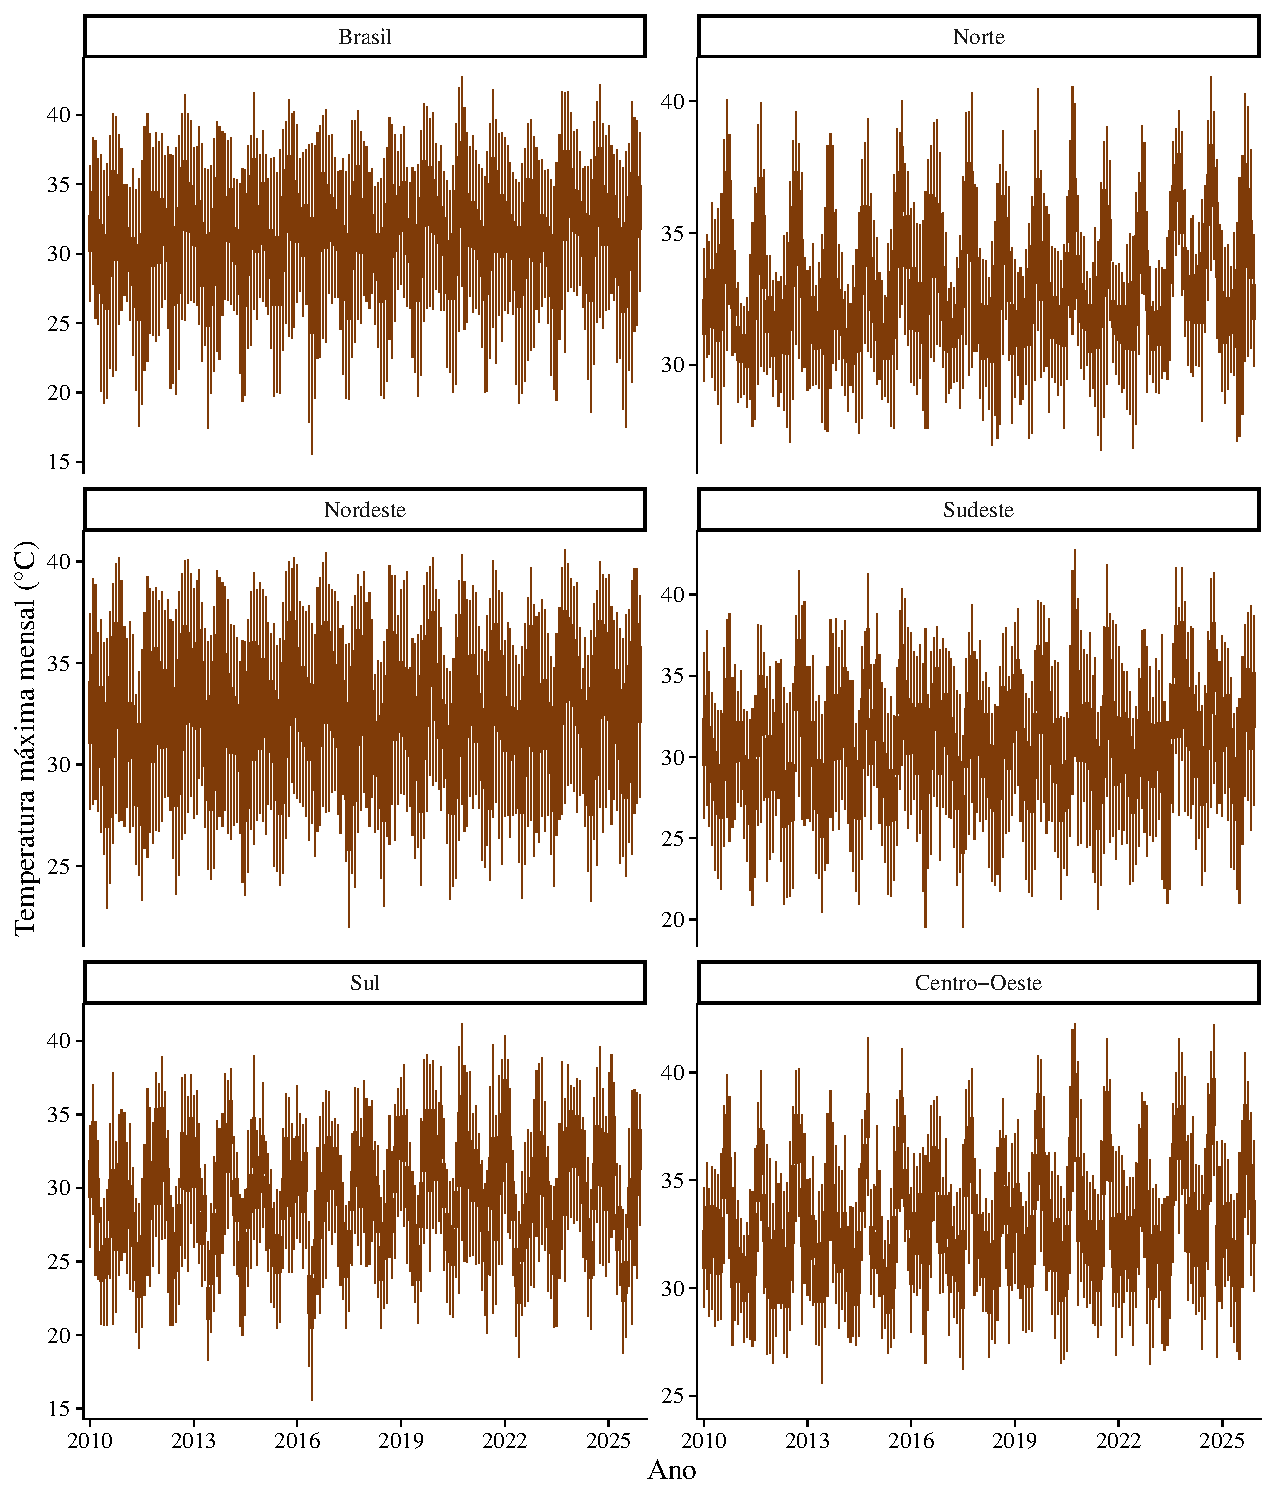
\includegraphics[width=0.95\textwidth]{fig_serie_boxplot_temperatura.pdf}
    \caption{Série mensal da temperatura máxima por Grande Região, Brasil, 2010--2025, em graus Celsius, com distribuição municipal resumida por mês. Fonte: reanálise climática.}
    \label{fig:serie_boxplot_temperatura}
\end{figure}

\subsection{Estratificação de risco e persistência epidêmica}
\label{subsec:resultados_estratificacao}

A Tabela~\ref{tab:estratificacao_risco} apresenta a distribuição dos \NumMunicipios{} municípios pelos estratos definidos para a razão acumulada de casos por população média: baixa (menos de 100 casos por 100 mil habitantes), média (100 a 300) e alta (mais de 300). No agregado nacional, \PctMunAltoRisco{} dos municípios ficaram no estrato alto, \PctMunMedioRisco{} no médio e \PctMunBaixoRisco{} no baixo. Nas regiões Sudeste e Centro-Oeste, praticamente todos os municípios enquadraram-se no estrato alto (99,9\% e 100,0\%, respectivamente), enquanto o Sul concentrou os de menor razão acumulada.

\begin{table}[!h]
\centering
\caption{\label{tab:estratificacao_risco}Distribuição dos municípios por estrato de risco e Grande Região, Brasil, 2010--2025.}
\centering
\resizebox{\ifdim\width>\linewidth\linewidth\else\width\fi}{!}{
\fontsize{9}{11}\selectfont
\begin{tabular}[t]{lcccccc}
\toprule
Estrato & Brasil & Norte & Nordeste & Sudeste & Sul & Centro-Oeste\\
\midrule
Baixa & 114 (2,0\%) & 8 (1,8\%) & 6 (0,3\%) & 0 (0,0\%) & 100 (8,4\%) & 0 (0,0\%)\\
Média & 254 (4,6\%) & 20 (4,5\%) & 42 (2,3\%) & 1 (0,1\%) & 191 (16,1\%) & 0 (0,0\%)\\
Alta & 5.196 (93,4\%) & 421 (93,8\%) & 1.745 (97,3\%) & 1.667 (99,9\%) & 897 (75,5\%) & 466 (100,0\%)\\
\bottomrule
\end{tabular}}
\end{table}


Na estratificação por tercis, as taxas por 100 mil pessoas-ano nos níveis 1 a 3 foram 797,6, 483,5 e 357,5 para esgotamento adequado; 821,7, 502,5 e 311,7 para abastecimento de água por rede; e 779,0, 526,8 e 305,5 para coleta de lixo. Para a densidade urbana, a taxa foi maior no nível intermediário (613,1; 768,4; e 649,2), enquanto para a proporção urbana aumentou entre os níveis (436,5; 558,3; e 732,8). Esses contrastes são descritivos e não estimam efeitos das covariáveis.

A Figura~\ref{fig:mapa_incidencia} apresenta a razão acumulada de casos por população média no período. \PctMunPersistencia{} dos municípios apresentaram dez ou mais anos com taxa anual acima de 300 por 100 mil habitantes, persistência mostrada na Figura~\ref{fig:mapa_persistencia}.

\begin{figure}[H]
    \centering
    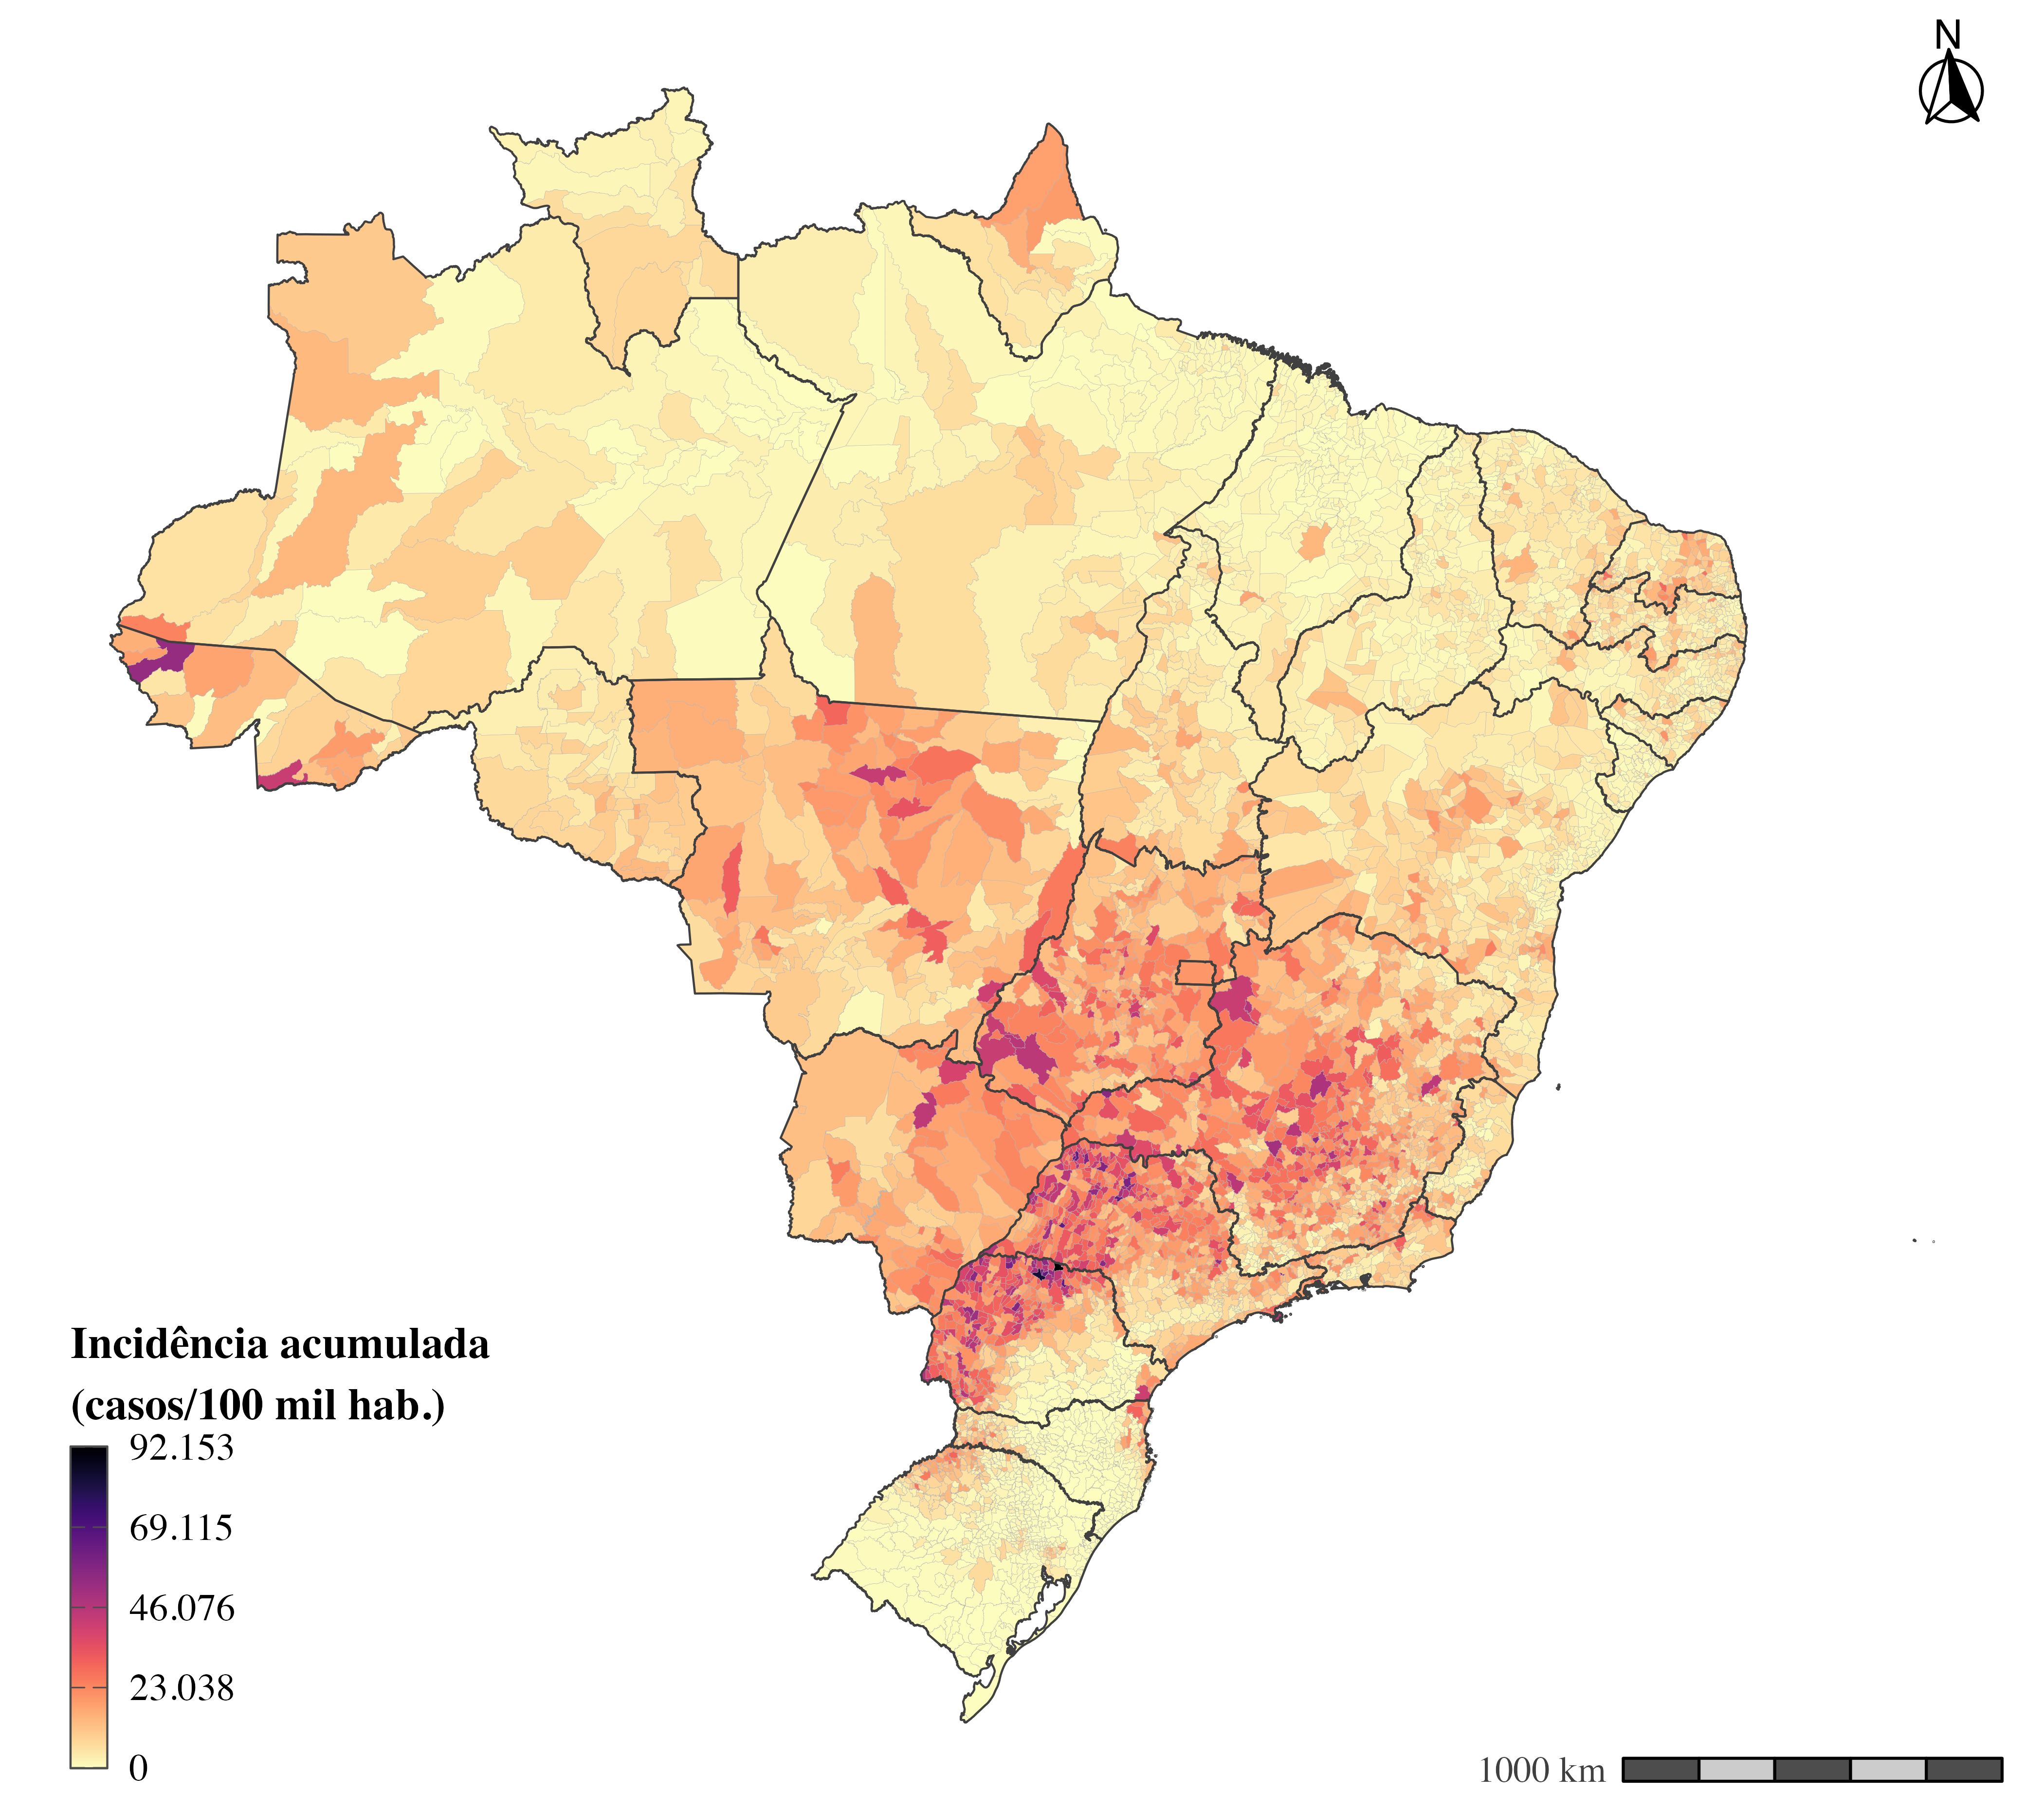
\includegraphics[width=0.76\textwidth]{fig_mapa_incidencia_acumulada.png}
    \caption{Razão acumulada de casos prováveis de dengue por população média municipal, Brasil, 2010--2025, expressa por 100 mil habitantes. Fontes: SINAN e IBGE.}
    \label{fig:mapa_incidencia}
\end{figure}

\begin{figure}[H]
    \centering
    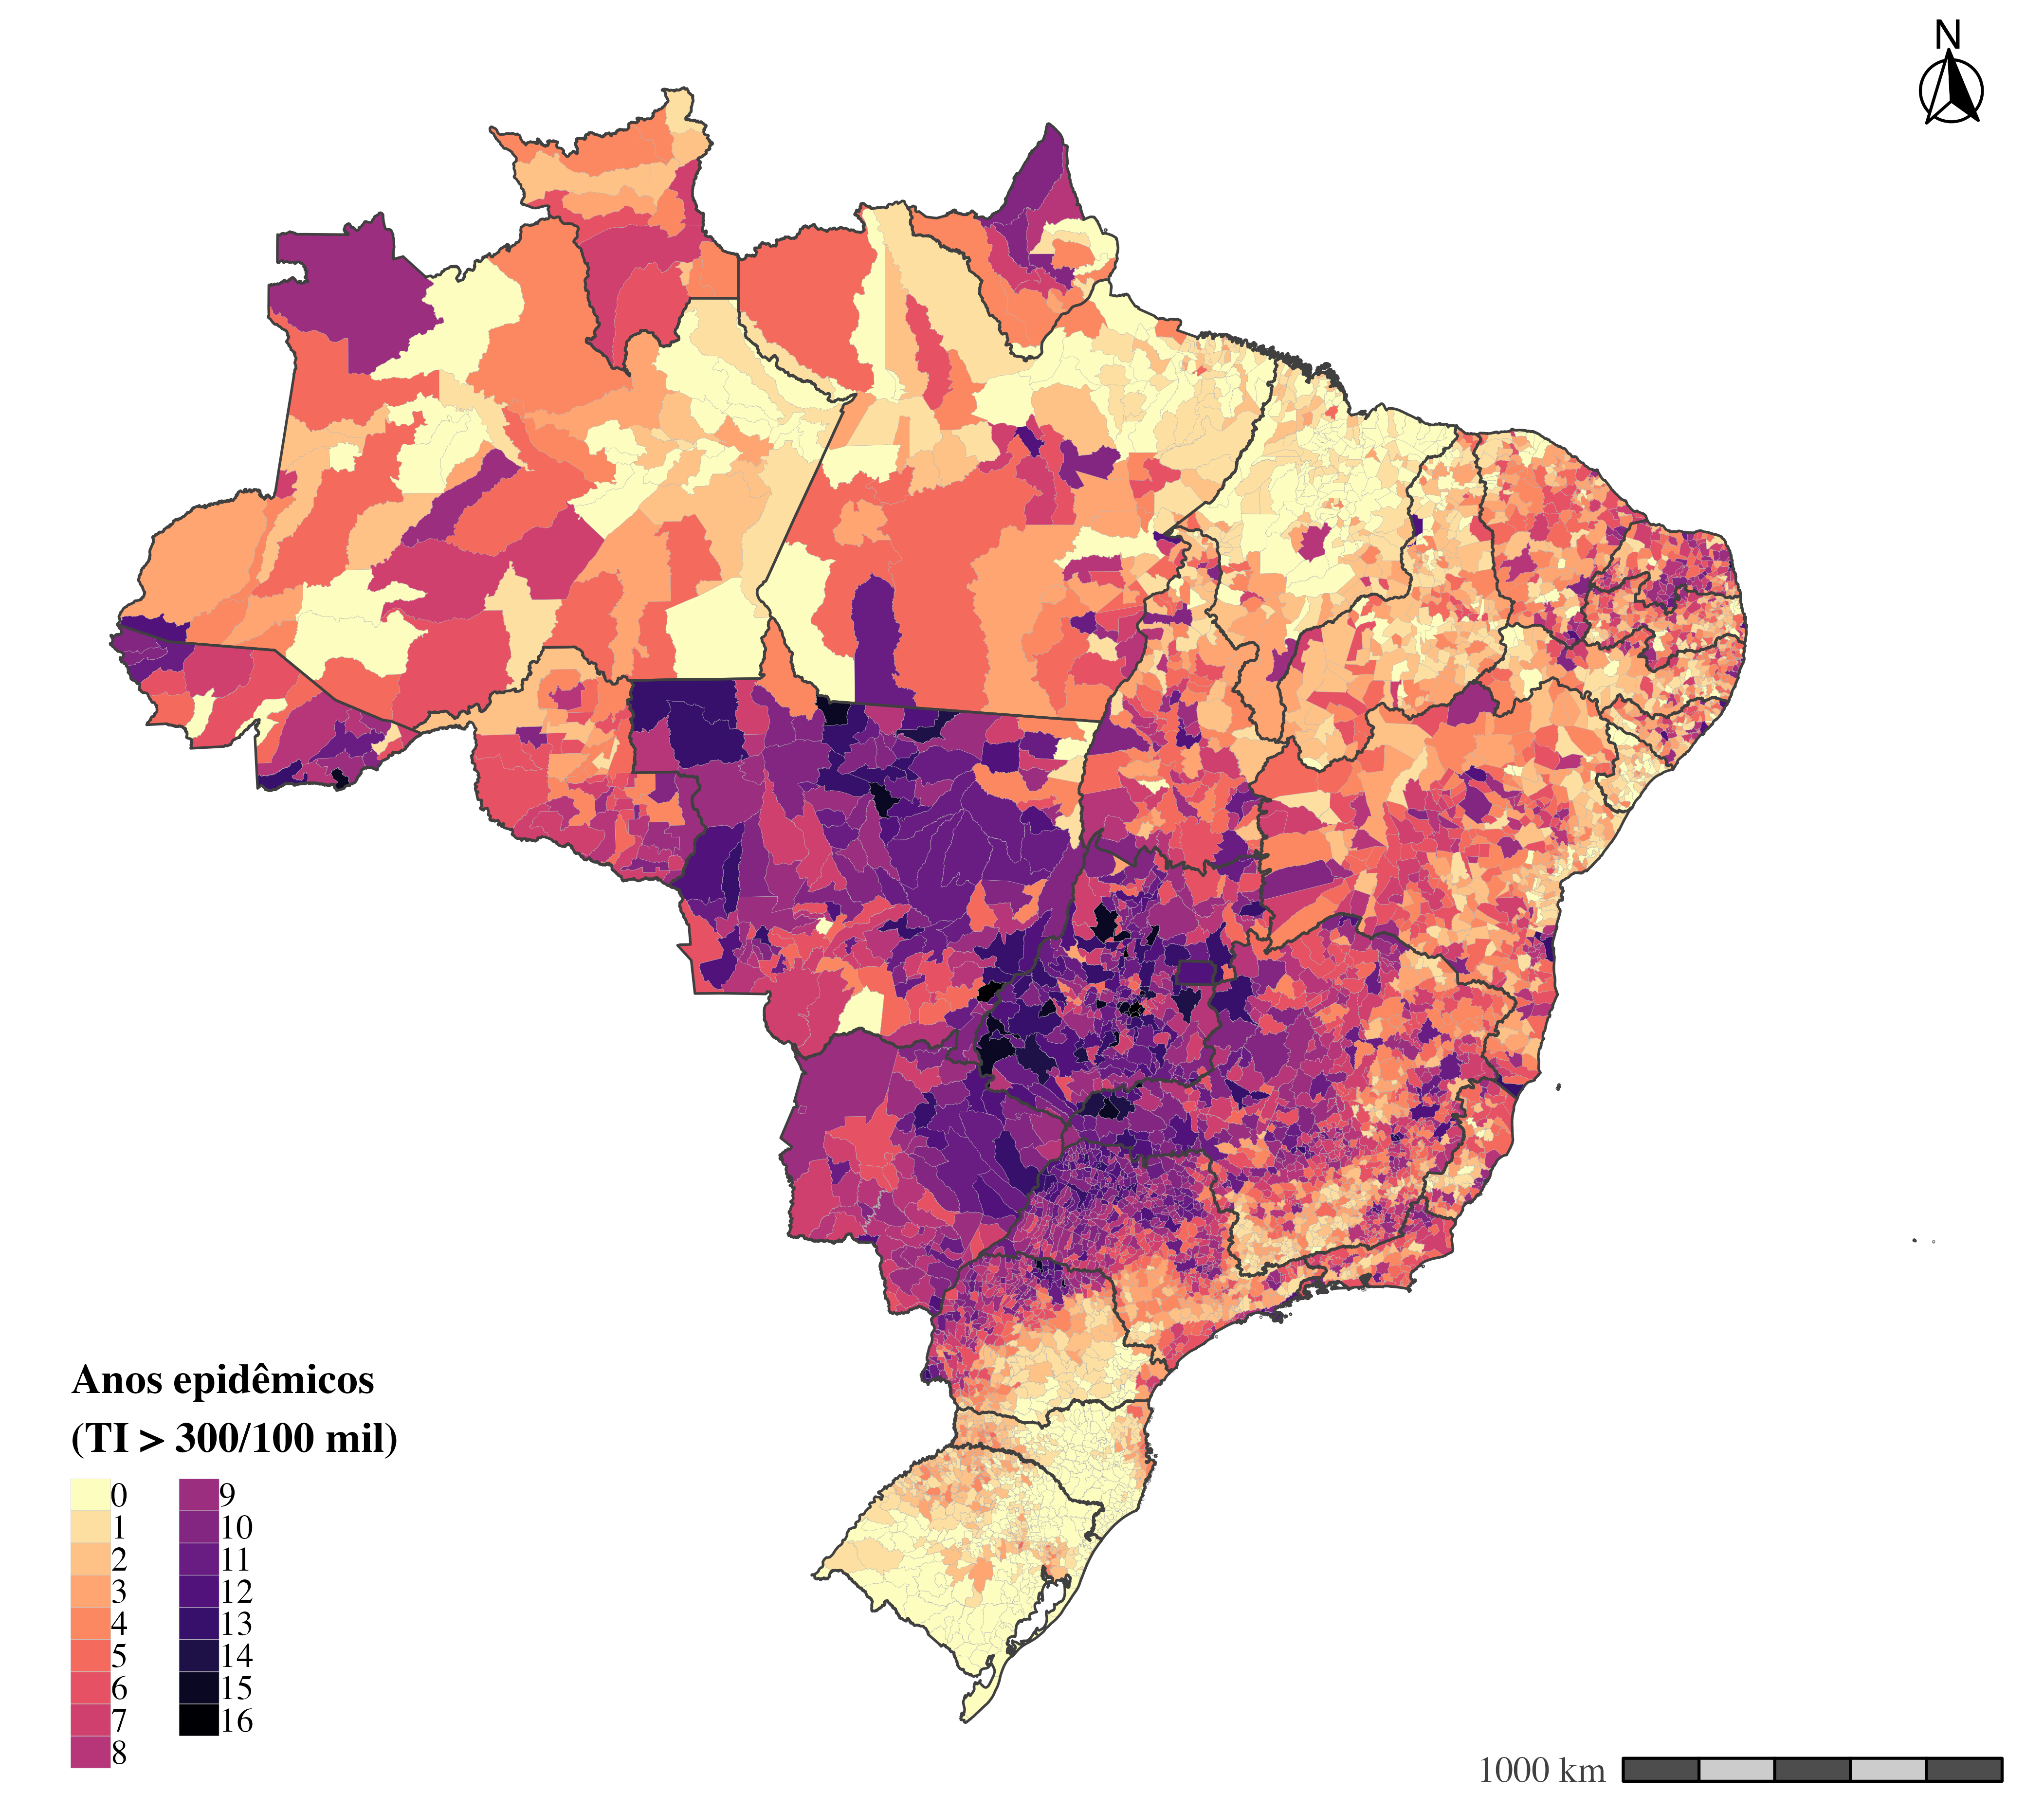
\includegraphics[width=0.76\textwidth]{fig_mapa_persistencia_epidemica.png}
    \caption{Número de anos, entre 2010 e 2025, com taxa de incidência acima de 300 casos por 100 mil habitantes, por município, Brasil. Fontes: SINAN e IBGE.}
    \label{fig:mapa_persistencia}
\end{figure}

Os quadrantes locais (Figura~\ref{fig:mapa_lisa}) mostram \textit{clusters} alto-alto entre Centro-Oeste e Sudeste e \textit{clusters} baixo-baixo na Amazônia Ocidental, em faixas do interior do Nordeste e no extremo Sul. A parcela sem associação local significativa foi de \LisaPctNS{}; a seção seguinte busca zonas de risco elevado pela estatística de varredura.

\section{Detecção e Análise de \textit{Clusters} Espaciais}
\label{sec:clusters}

A varredura espacial usou os \ScanTotalCasos{} casos do painel e a população média residente (\ScanPopulacao{} habitantes). Os casos de 2024 representam 29,1\% do total acumulado, de modo que a varredura reflete esse ano epidêmico. A comparação entre as oito formulações é descritiva e exploratória: o método delimita zonas de excesso, e não estima efeitos como uma regressão. Antes da apresentação detalhada dos \textit{clusters}, o modelo sem ajuste e os sete ajustes são confrontados quanto ao número e à posição das zonas, ao erro absoluto percentual ponderado e à sobreposição municipal; essa comparação orienta a leitura das subseções seguintes.

\subsection{Comparação entre as oito formulações}
\label{subsec:satscan_sensibilidade}

Cada formulação gerou uma coleção própria de zonas e uma distribuição própria de casos esperados municipais. A Tabela~\ref{tab:comparacao_satscan} resume os resultados. As coleções variaram de 128 (calor) a 195 (lixo) zonas significativas, com cobertura entre 62,5\% e 64,9\% dos casos do painel. O polo primário permaneceu no Centro-Sul em todas as formulações, com deslocamento entre Adolfo (SP) no modelo sem ajuste, Queluzito (MG) sob calor, Iacri (SP) sob esgoto, proporção urbana, água e lixo, e Araújos (MG) sob densidade urbana e índice composto. O WMAPE, que resume a proximidade entre esperado padronizado e observado, caiu de 75,1\% sem ajuste para 64,9\% sob calor, 70,5\% sob água, 71,9\% sob esgoto, 71,9\% sob o índice composto, 72,1\% sob lixo, 74,3\% sob densidade urbana e 74,4\% sob proporção urbana. A sobreposição municipal com o modelo sem ajuste (índice de Jaccard) ficou entre 56\% (calor) e 82\% (densidade urbana). Em nenhuma formulação a redução do WMAPE foi acompanhada do desaparecimento das zonas de excesso.

\begin{table}[!h]
\centering
\caption{\label{tab:comparacao_satscan}Comparação dos ajustes por covariáveis na varredura espacial: zonas significativas, polo primário, risco relativo, cobertura de casos e WMAPE nacional, Brasil, 2010--2025.}
\centering
\resizebox{\ifdim\width>\linewidth\linewidth\else\width\fi}{!}{
\fontsize{9}{11}\selectfont
\begin{tabular}[t]{lclcccc}
\toprule
Ajuste & Zonas & Primário (polo) & $RR$ & \% dos casos & WMAPE (\%) & Redução (p.p.)\\
\midrule
Sem ajuste & 129 & Adolfo (SP) & 2,99 & 64,1\% & 75,1 & —\\
Calor & 128 & Queluzito (MG) & 2,08 & 63,3\% & 64,9 & 10,2\\
Esgoto adequado & 178 & Iacri (SP) & 2,79 & 64,0\% & 71,9 & 3,2\\
Densidade urbana & 136 & Araújos (MG) & 2,73 & 63,2\% & 74,3 & 0,8\\
Proporção urbana & 158 & Iacri (SP) & 3,11 & 63,3\% & 74,4 & 0,6\\
\addlinespace
Água por rede & 193 & Iacri (SP) & 2,70 & 63,4\% & 70,5 & 4,6\\
Coleta de lixo & 195 & Iacri (SP) & 2,86 & 64,9\% & 72,1 & 3,0\\
Índice composto & 184 & Araújos (MG) & 2,58 & 62,5\% & 71,9 & 3,2\\
\bottomrule
\end{tabular}}
\end{table}


O ajuste por tercis de dias em onda de calor combinou a maior redução do WMAPE (de 75,1\% para 64,9\%, 10,2 pontos percentuais) com a manutenção de uma coleção extensa de zonas residuais, razão pela qual as subseções seguintes detalham o modelo sem ajuste e o ajuste por calor.

\subsection{Consistência das zonas entre as formulações}

Para resumir a robustez das zonas às diferentes estratificações, a Figura~\ref{fig:robustez} classifica cada município pelo número de formulações (o modelo sem ajuste e os sete ajustes, de uma a oito) em que ele pertence a uma zona significativa, sobrepondo as coleções de todos os modelos. Dos 5.564 municípios do painel, 3.016 (54,2\%) aparecem em pelo menos uma formulação, 1.655 (29,7\%) em seis ou mais e 967 (17,4\%) em todas as oito; 378 municípios aparecem em apenas uma. Os tons mais escuros concentram-se no Centro-Sul, sobretudo no Sudeste e no Centro-Oeste, enquanto a maior parte do Norte e do interior do Nordeste permanece fora de zonas ou em poucas formulações. A leitura é de robustez às formulações, e não de intensidade de risco: aparecer em todas elas indica que o excesso se mantém sob qualquer um dos esquemas de padronização testados, ao passo que aparecer em poucas acompanha os excessos marginais descritos no modelo sem ajuste. 
\begin{figure}[H]
    \centering
    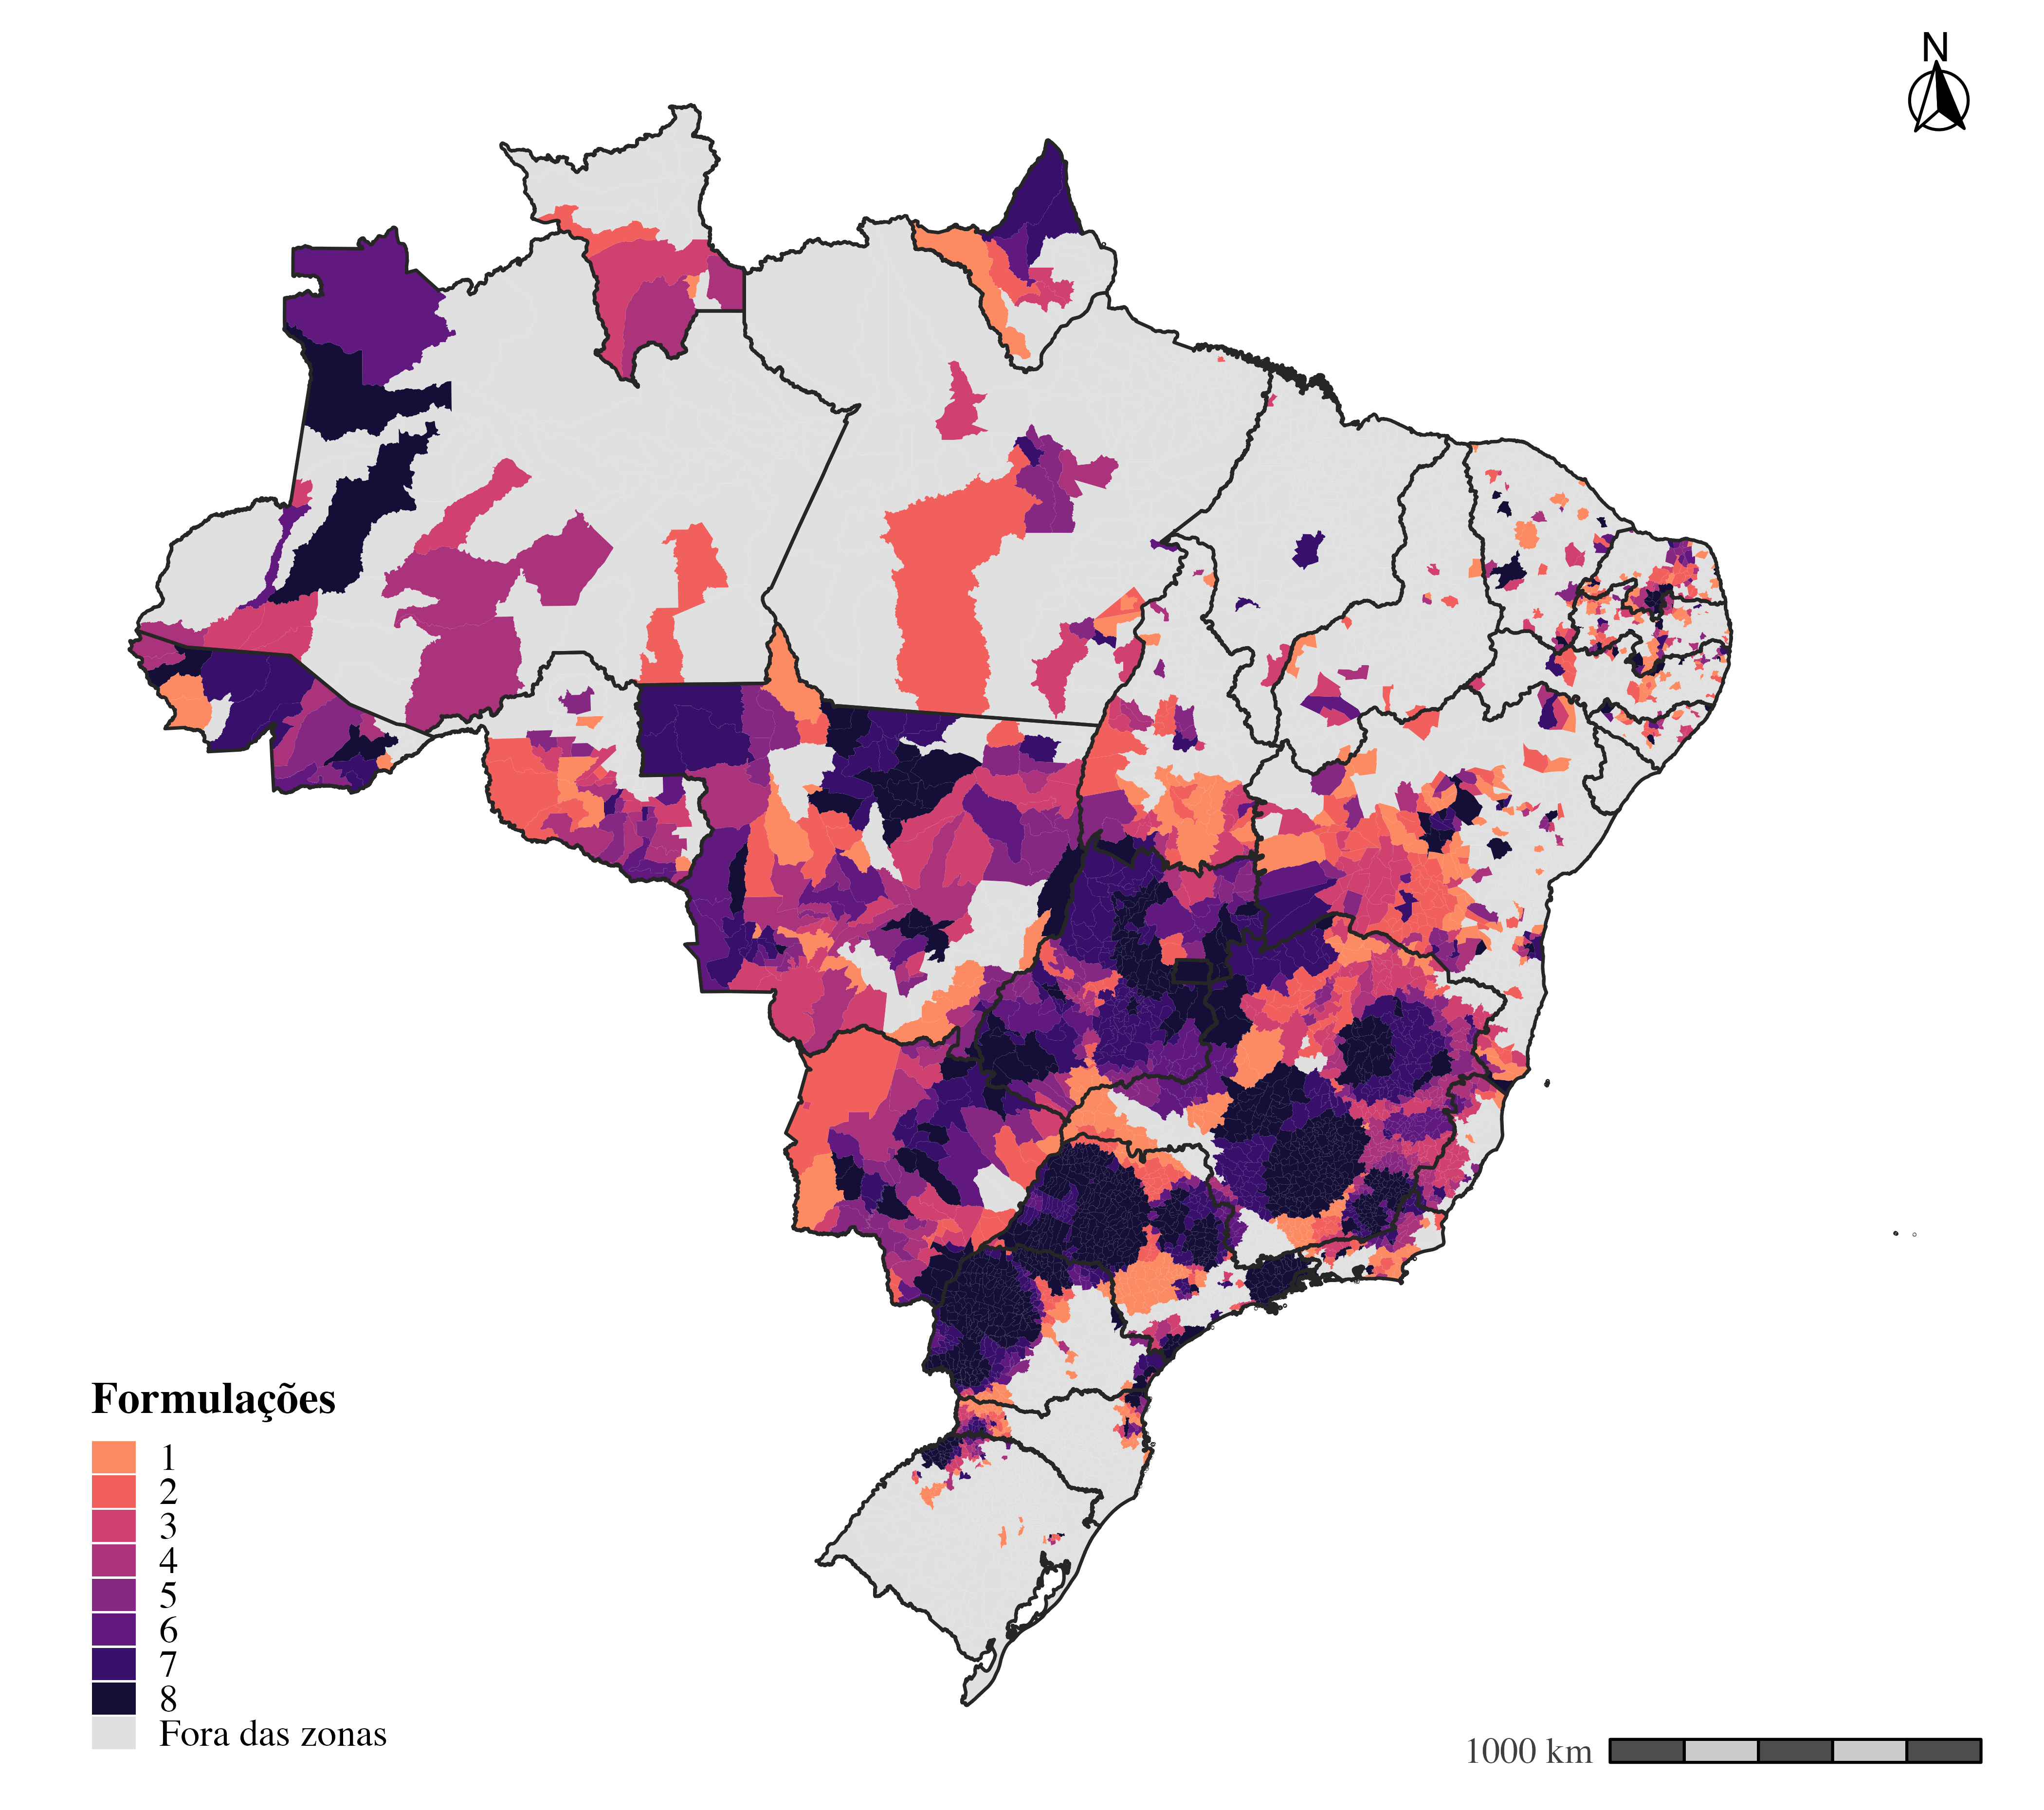
\includegraphics[width=0.76\textwidth]{fig_mapa_persistencia_ajustes.png}
    \caption{Consistência das zonas significativas de alto risco entre as formulações da varredura espacial, Brasil, 2010--2025: número de formulações, de uma a oito, em que cada município pertence a uma zona. Fontes: SINAN e IBGE.}
    \label{fig:robustez}
    \vspace{0.3em}
    {\footnotesize\noindent\textit{Nota:} Tons mais escuros indicam presença em mais formulações, no gradiente discreto de uma a oito; em cinza, municípios que não pertencem a zonas em nenhuma das oito formulações.\par}
\end{figure}

\subsection{Modelo sem ajuste}
\label{subsec:satscan_puro}

Com limite de 16\% da população e 200~km de raio, o modelo sem ajuste reteve 129 zonas sem sobreposição (nível de 5\%), que recobriram \ScanCobMunicipios{} municípios (\ScanCobMunicipiosPct{} dos municípios) e concentraram \ScanCobCasos{} casos (\ScanCobCasosPct{} dos casos do painel) em \ScanCobPopPct{} da população sob risco. Das 129 zonas significativas, 16 apresentam risco relativo abaixo de 1,2 e 70 abaixo de 1,5, de modo que parte da coleção corresponde a excessos marginais\footnote{Isto é, zonas cujo risco relativo é pouco maior que 1; a significância dessas zonas decorre sobretudo do volume acumulado sob o modelo de Poisson.}. A Figura~\ref{fig:mapas_zonas} mostra a extensão dessas zonas (painel a) e a coleção do ajuste por calor (painel b), para comparação; a Figura~\ref{fig:mapas_rr} usa os mesmos dois modelos para o risco relativo municipal.

O \textit{cluster} primário centrou-se em Adolfo (SP), com \ScanPrimMunicipios{} municípios em um raio de \ScanPrimRaioKm{}~km, \ScanPrimCasosObs{} casos observados contra \ScanPrimCasosEsp{} esperados, risco relativo de $RR = \ScanPrimRR{}$ ($p \ScanPrimPValor{}$; razão de verossimilhança logarítmica (LLR) $= \ScanPrimLLR{}$), abrangendo \ScanPrimPop{} habitantes (\ScanPrimPopPct{} da população) e \ScanPrimCasosPct{} dos casos. O segundo aglomerado centrou-se em Araújos (MG), com 229 municípios em raio de 199,8~km ($RR = 2{,}74$; 2.588.779 casos observados contra 1.019.064 esperados), seguido por Palmelo (GO), com 122 municípios em raio de 198,1~km ($RR = 2{,}54$; 2.259.957 casos contra 948.039 esperados). O maior risco relativo da coleção ocorreu em Cruzeiro do Sul (AC), zona unimunicipal com $RR = 4{,}95$ (46.111 casos). Nenhum raio primário ou secundário excede 200~km, consistente com o limite. A lista completa das 129 zonas consta do Apêndice~\ref{app:clusters}.

\begin{figure}[H]
    \centering
    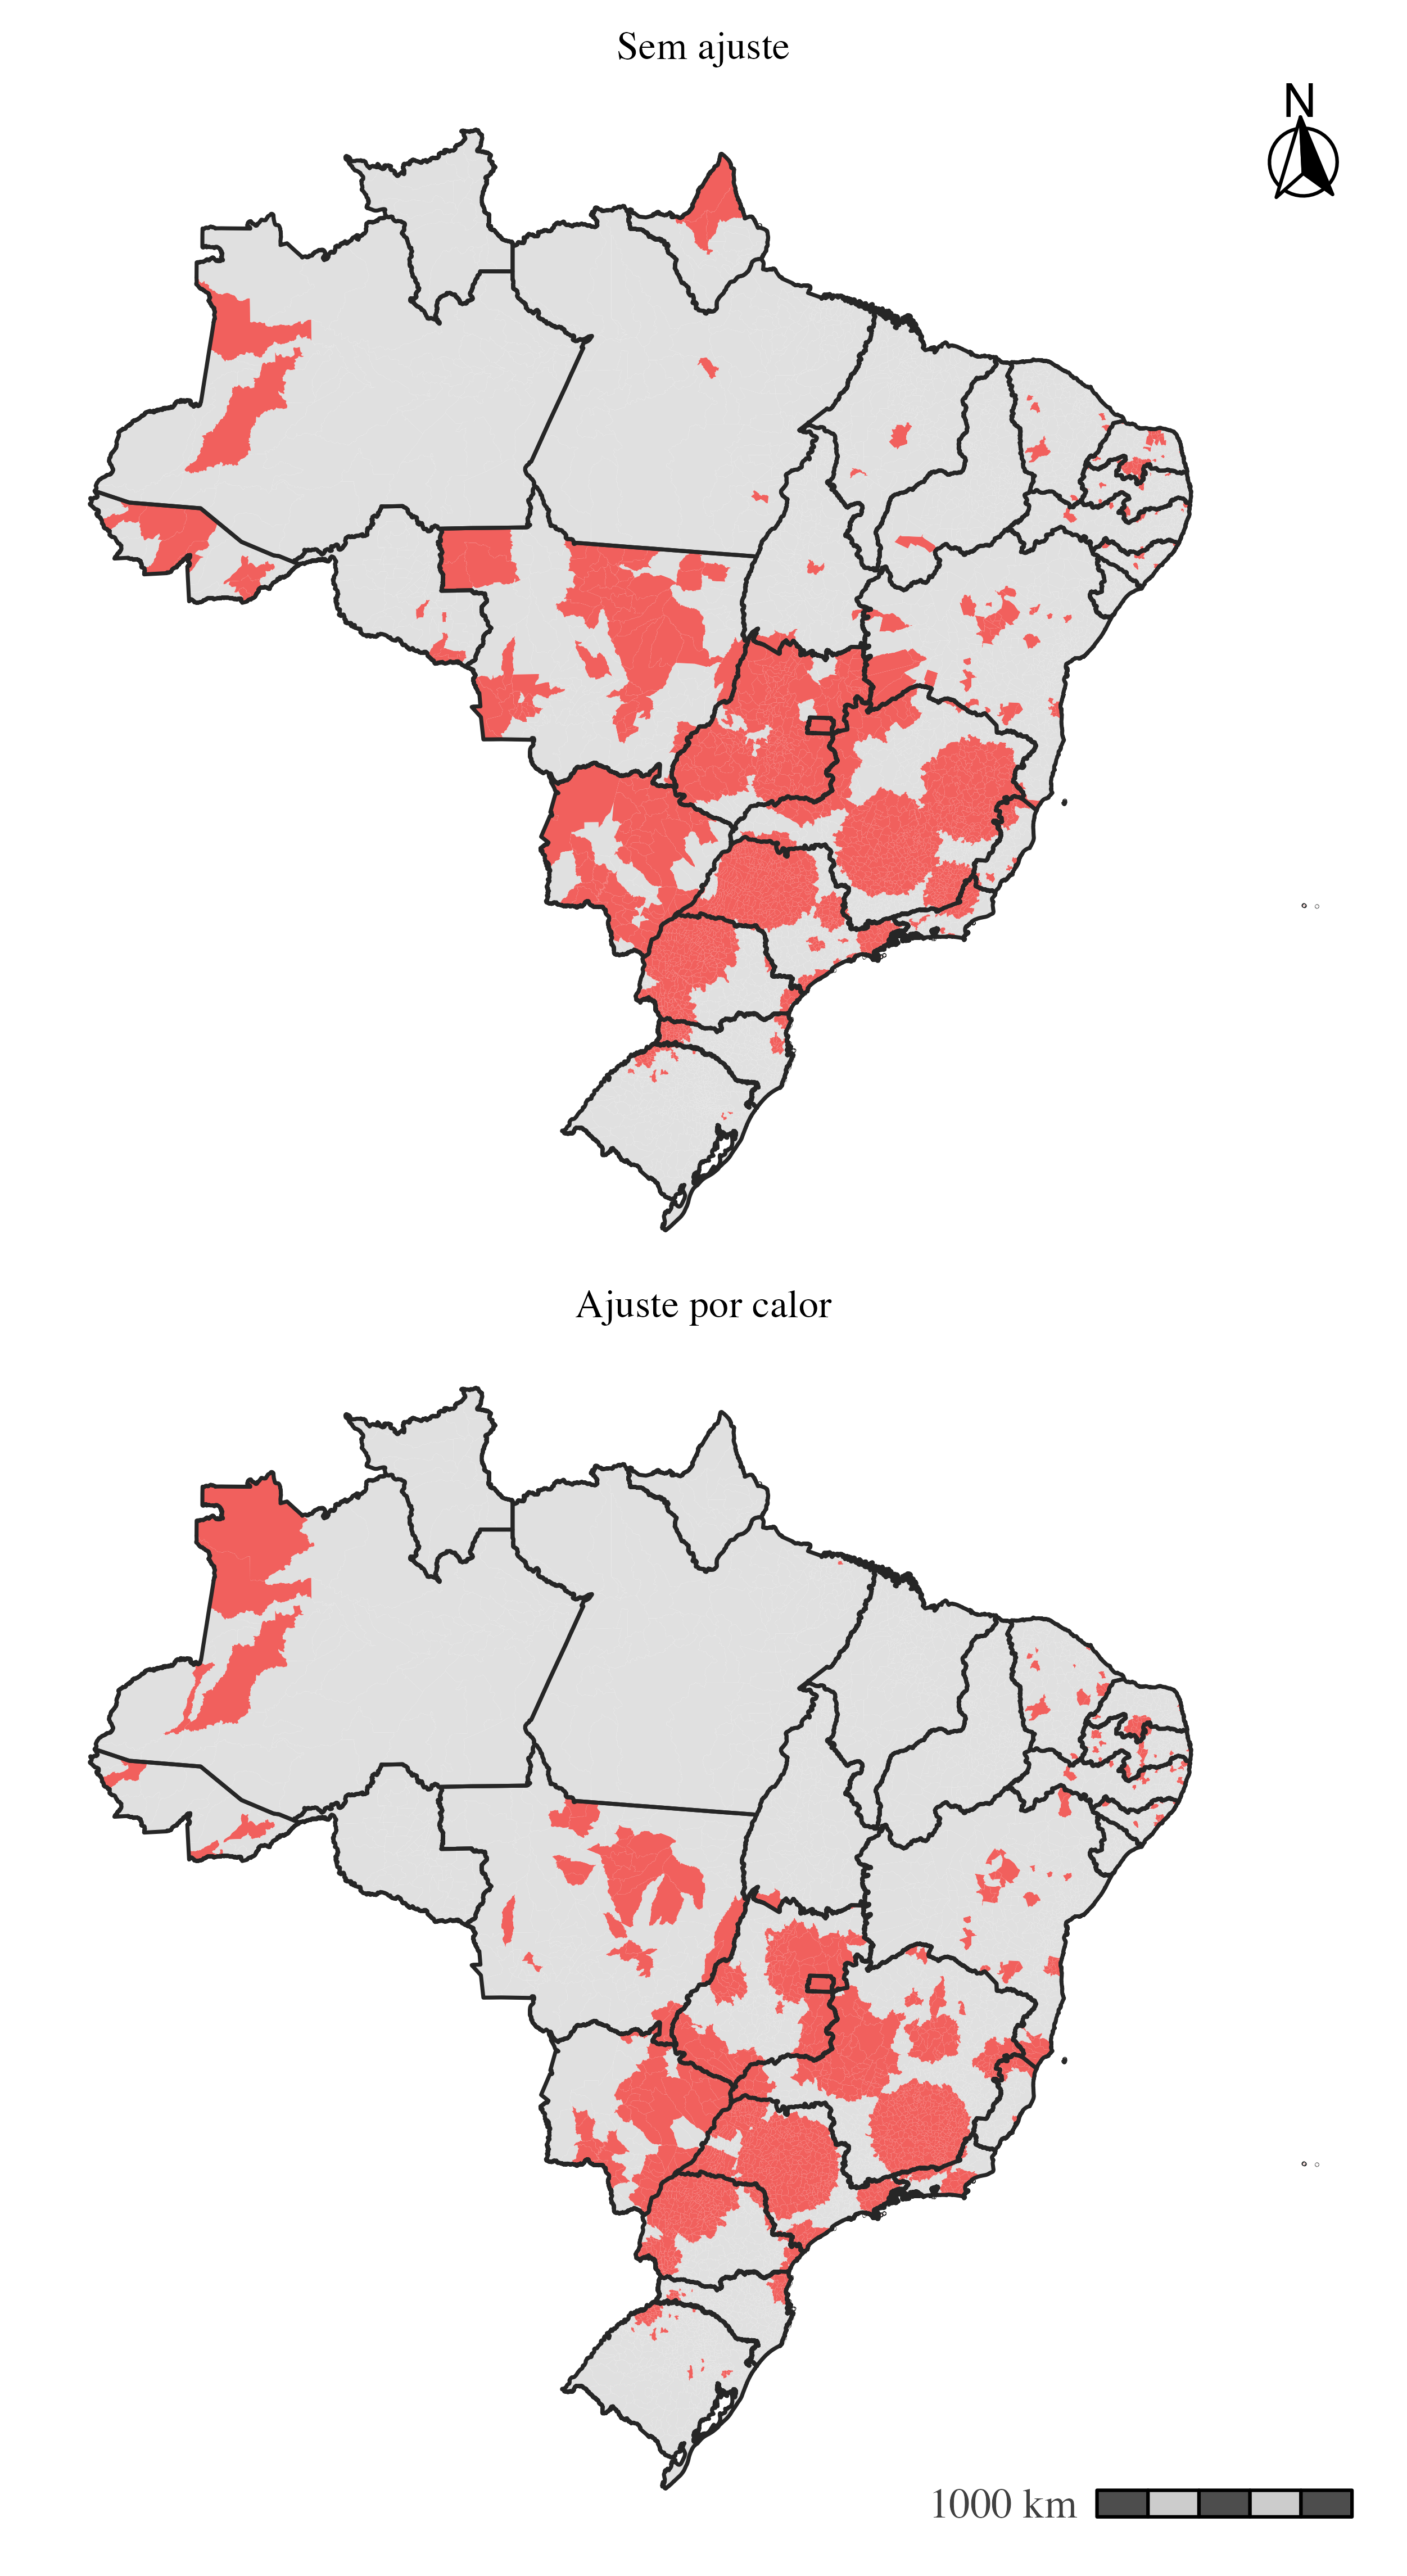
\includegraphics[width=0.66\textwidth]{fig_mapa_clusters_2x1_puro_calor.png}
    \caption{Zonas significativas de alto risco de dengue, Brasil, 2010--2025. (a) Sem ajuste. (b) Ajuste por calor. O modelo sem ajuste identificou 129 zonas sem sobreposição (nível de 5\%), com primário em Adolfo (SP), 319 municípios e risco relativo de 2,99, cobrindo 64,1\% dos casos do painel. O ajuste por calor identificou 128 zonas, com primário em Queluzito (MG), 362 municípios e risco relativo de 2,08, cobrindo 63,3\% dos casos. Fontes: SINAN e IBGE.}
    \label{fig:mapas_zonas}
    \vspace{0.3em}
    {\footnotesize\noindent\textit{Nota:} Em laranja, municípios em zonas com nível de 5\%; em cinza, municípios fora de zonas. Valores de casos, expectativa e risco relativo para 2010--2025.\par}
\end{figure}

\begin{figure}[H]
    \centering
    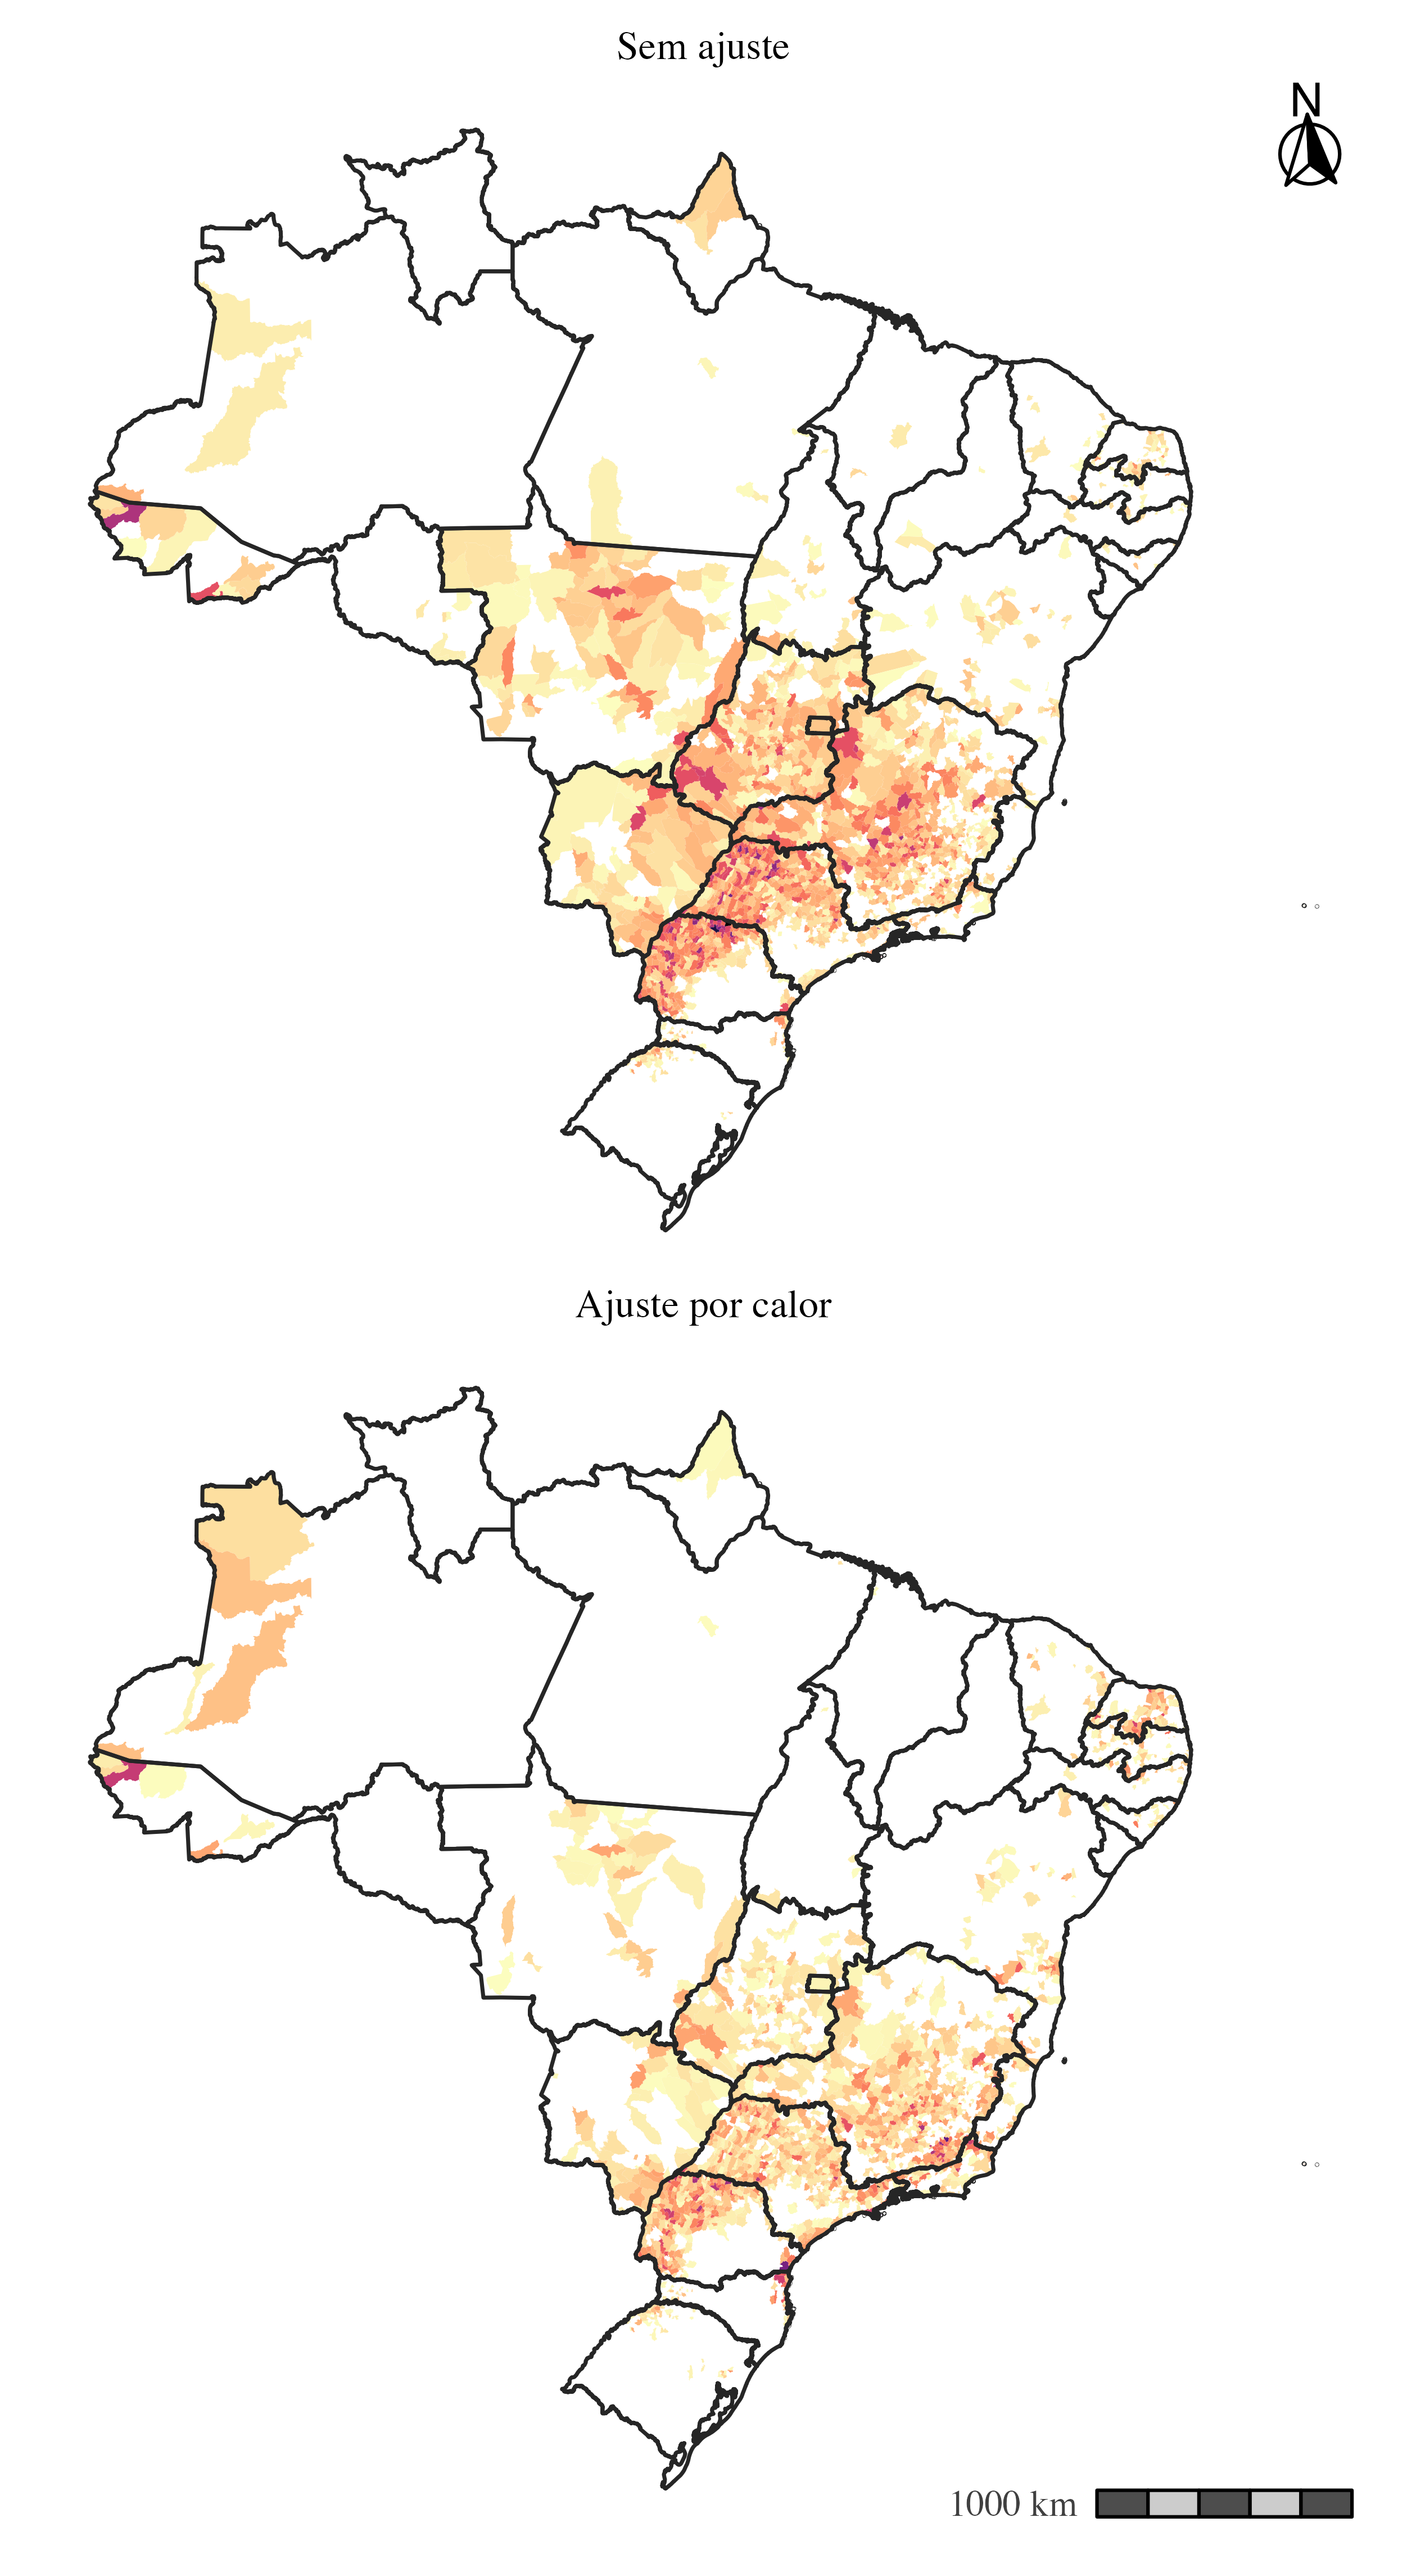
\includegraphics[width=0.66\textwidth]{fig_mapa_rr_2x1_puro_calor.png}
    \caption{Risco relativo municipal estimado pela varredura espacial sem ajuste (a) e sob ajuste por calor (b), Brasil, 2010--2025. Fontes: SINAN e IBGE.}
    \label{fig:mapas_rr}
    \vspace{0.3em}
    {\footnotesize\noindent\textit{Nota:} Tons mais escuros indicam risco relativo mais alto, na escala comum aos dois painéis, de 1,0 a 8,6; em branco, municípios com $RR \le 1{,}0$. O risco relativo é o reportado pelo programa sob a expectativa padronizada de cada modelo.\par}
\end{figure}

\subsection{Ajuste por calor}
\label{subsec:satscan_calor}

O ajuste por tercis de dias em onda de calor reteve 128 zonas, com cobertura de 1.679 municípios (30,2\%) e 13.989.139 casos (63,3\%) em 31,5\% da população. O primário deslocou-se para Queluzito (MG), com 362 municípios em raio de 199,5~km e $RR = 2{,}08$ (2.967.585 casos contra 1.533.663 esperados), seguido por Boracéia (SP), com 335 municípios ($RR = 1{,}86$), e por Goiânia (GO), janela compacta de 3 municípios em 18,8~km ($RR = 2{,}40$; 810.059 casos contra 344.386 esperados). A lista completa das 128 zonas consta do Apêndice~\ref{app:clusters_termica}.

As Figuras~\ref{fig:mapas_zonas} e \ref{fig:mapas_rr} comparam o modelo sem ajuste e o ajuste por calor. As Figuras~\ref{fig:prancha_clusters}, \ref{fig:prancha_clusters_sem2024} e \ref{fig:prancha_rr}, reunidas no Apêndice~\ref{app:pranchas}, apresentam, respectivamente, as zonas significativas das oito formulações no período completo, as zonas no cenário sem 2024 e os riscos relativos das seis formulações restantes. As Tabelas~\ref{tab:clusters_satscan_puro} e \ref{tab:clusters_satscan_termica}, nos Apêndices~\ref{app:clusters} e \ref{app:clusters_termica}, detalham as zonas municipais dos modelos sem ajuste e com ajuste por calor.

\subsection{Sensibilidade à exclusão de 2024}
\label{subsec:satscan_sens2024}

Para avaliar a sensibilidade ao ano epidêmico de 2024, as oito formulações foram reexecutadas sem os casos desse ano, com configuração idêntica (Figuras~\ref{fig:zonas_puro_2024} e \ref{fig:zonas_calor_2024}). A Tabela~\ref{tab:sensibilidade_satscan} apresenta o número de zonas, o polo primário e a sobreposição municipal entre os cenários. Sem 2024, o painel reúne 15.664.546 casos e o número de zonas significativas aumentou sem ajuste (de 129 para 169), sob calor (de 128 para 130), sob densidade urbana (de 136 para 168), sob proporção urbana (de 158 para 173) e sob o índice composto (de 184 para 196); sob esgoto, água e lixo, diminuiu ligeiramente. O polo primário sem ajuste deslocou-se de Adolfo (SP) para Ubarana (SP) e, sob calor, de Queluzito (MG) para Iacri (SP). A sobreposição municipal entre os cenários variou de 51\% (calor) a 63\% (esgoto). O WMAPE foi maior no cenário sem 2024 em todas as formulações (por exemplo, 81,0\% sem ajuste e 71,0\% sob calor), mas a ordenação relativa no topo foi preservada: calor e água permaneceram os menores valores nos dois cenários.

\begin{table}[!h]
\centering
\caption{\label{tab:sensibilidade_satscan}Sensibilidade à exclusão de 2024 na varredura espacial: número de zonas, polo primário e sobreposição municipal entre os cenários (2010--2025 e sem 2024), Brasil.}
\centering
\resizebox{\ifdim\width>\linewidth\linewidth\else\width\fi}{!}{
\fontsize{9}{11}\selectfont
\begin{tabular}[t]{lccllc}
\toprule
\multicolumn{1}{c}{ } & \multicolumn{2}{c}{Zonas (n)} & \multicolumn{2}{c}{Polo primário} & \multicolumn{1}{c}{Sobreposição entre cenários} \\
\cmidrule(l{3pt}r{3pt}){2-3} \cmidrule(l{3pt}r{3pt}){4-5} \cmidrule(l{3pt}r{3pt}){6-6}
Ajuste & Com 2024 & Sem 2024 & Com 2024 & Sem 2024 & Jaccard\\
\midrule
Sem ajuste & 129 & 169 & Adolfo (SP) & Ubarana (SP) & 61\%\\
Calor & 128 & 130 & Queluzito (MG) & Iacri (SP) & 51\%\\
Esgoto adequado & 178 & 174 & Iacri (SP) & Iacri (SP) & 63\%\\
Densidade urbana & 136 & 168 & Araújos (MG) & Ubarana (SP) & 55\%\\
Proporção urbana & 158 & 173 & Iacri (SP) & Ubarana (SP) & 58\%\\
\addlinespace
Água por rede & 193 & 188 & Iacri (SP) & Ubarana (SP) & 60\%\\
Coleta de lixo & 195 & 186 & Iacri (SP) & Ubarana (SP) & 60\%\\
Índice composto & 184 & 196 & Araújos (MG) & Ubarana (SP) & 61\%\\
\bottomrule
\end{tabular}}
\end{table}


\clearpage
\begin{figure}[H]
    \centering
    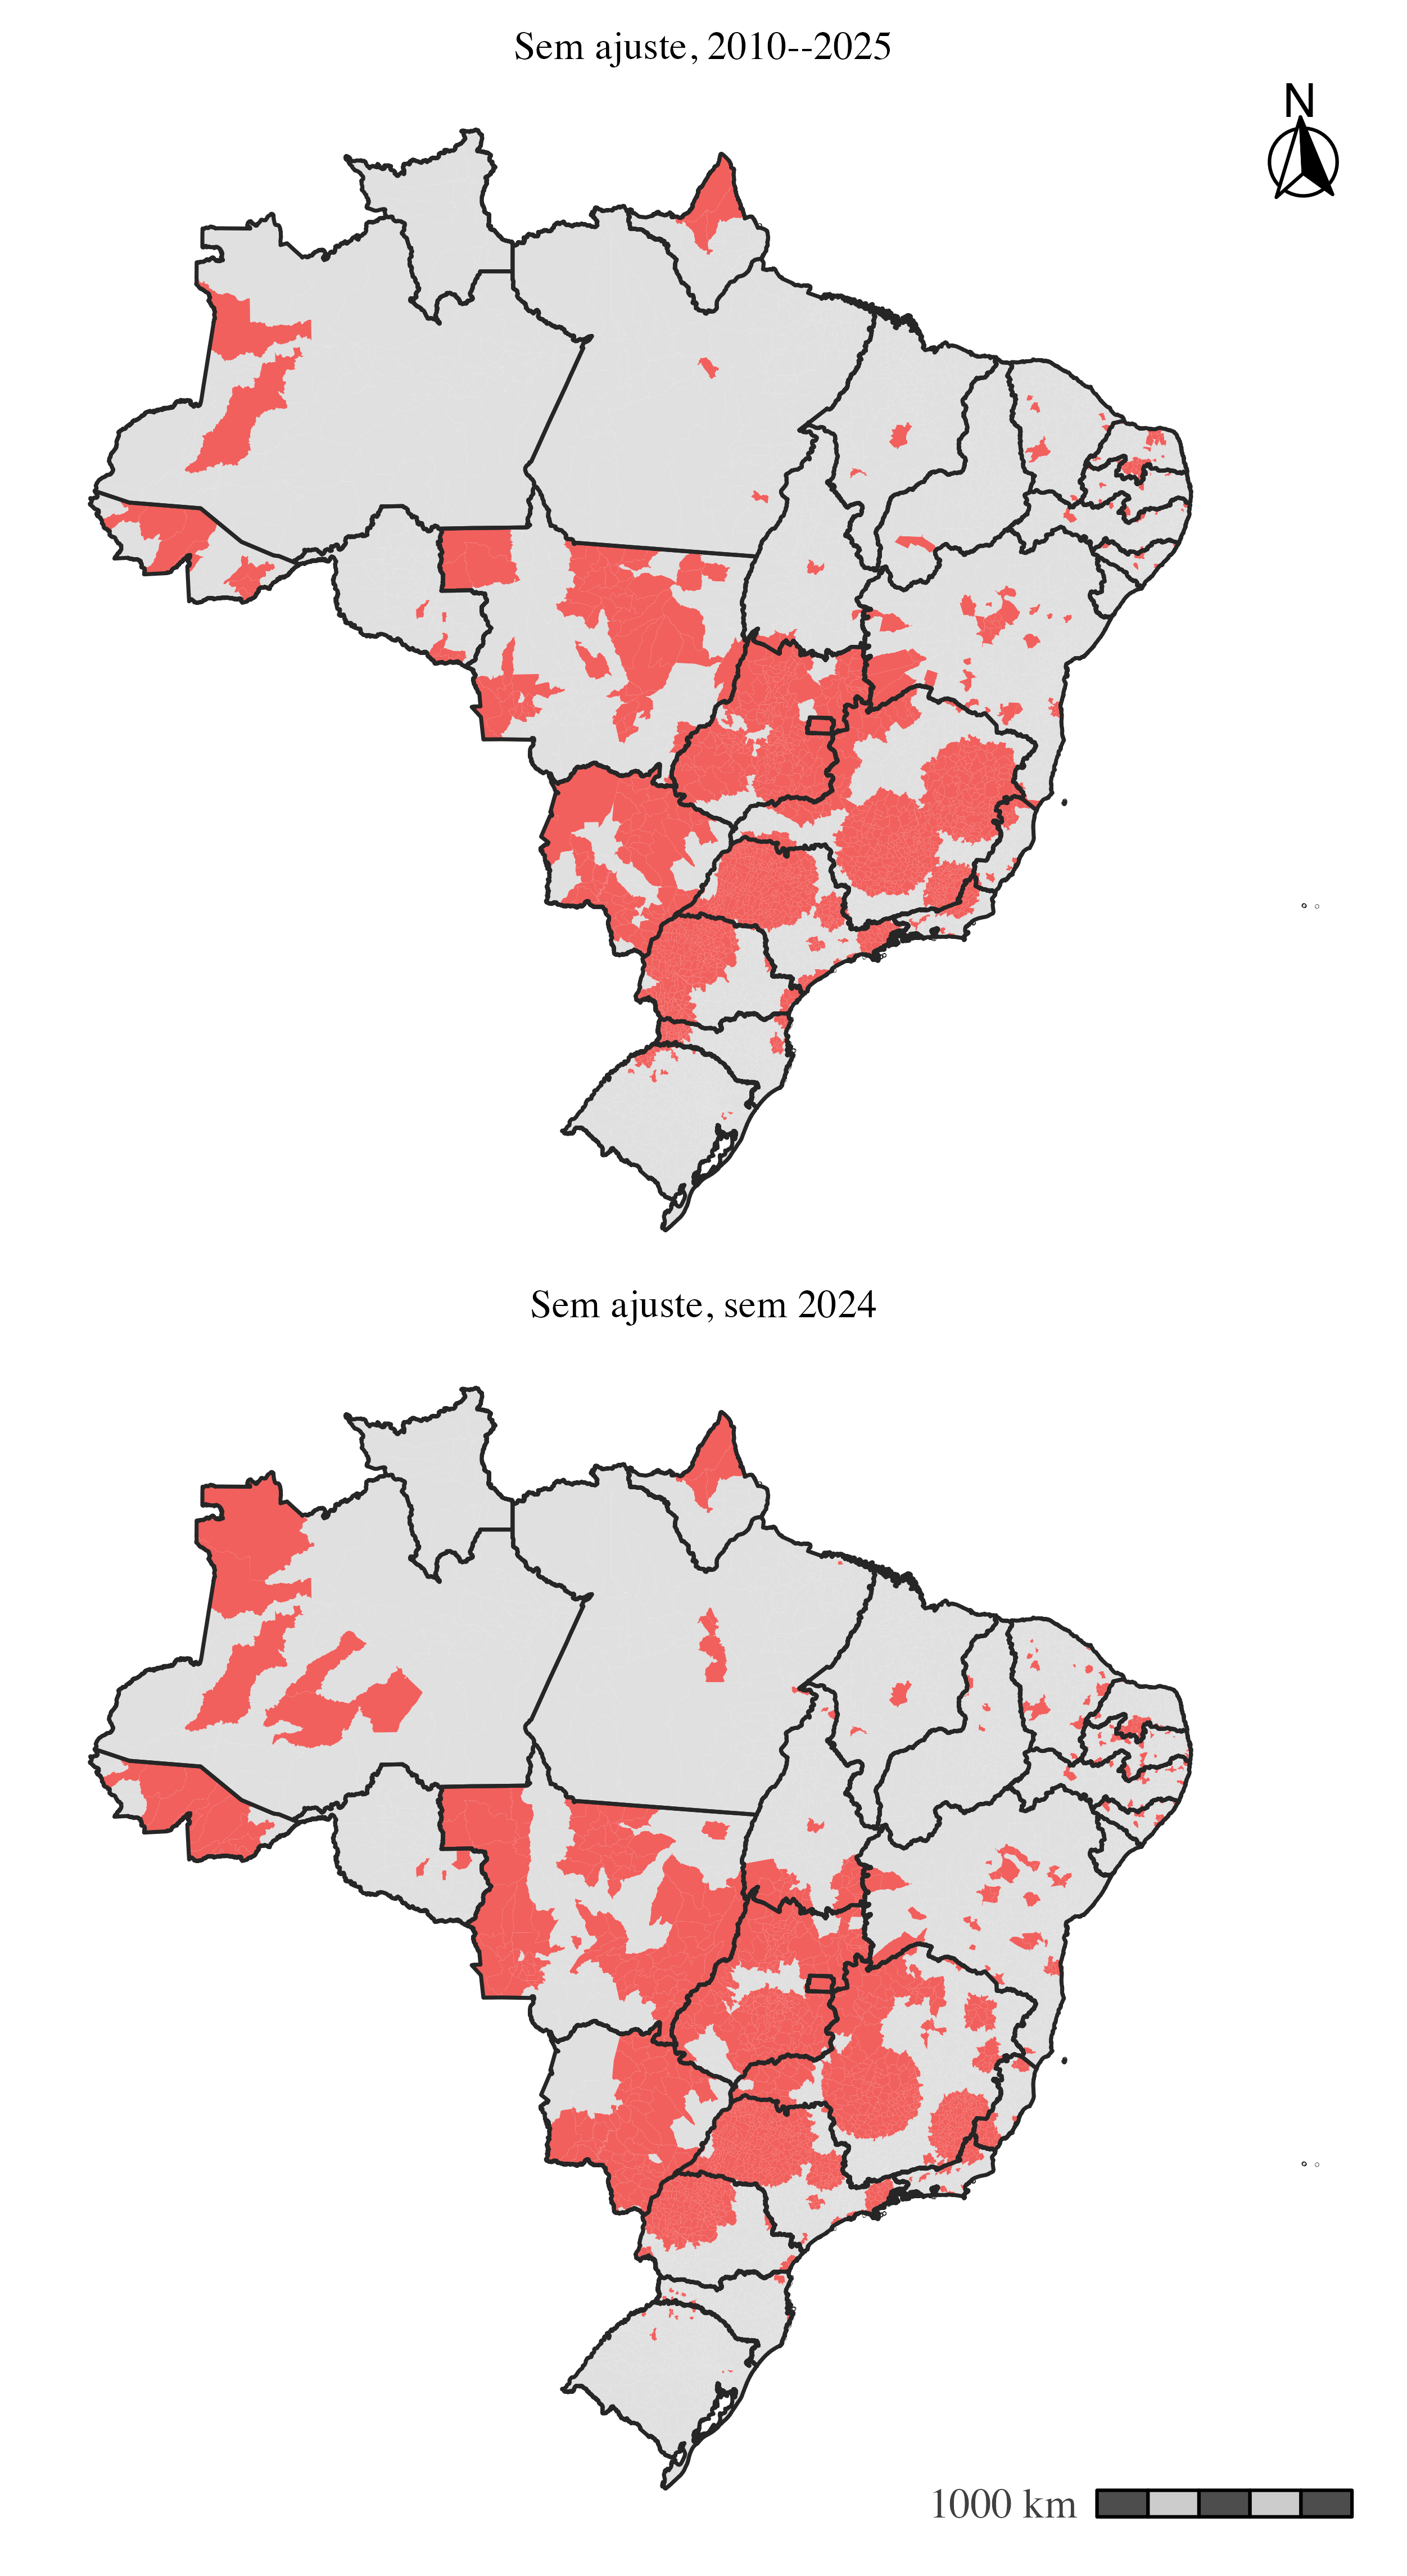
\includegraphics[width=0.66\textwidth]{fig_mapa_clusters_2x1_puro_com_sem2024.png}
    \caption{Zonas de alta incidência no modelo sem ajuste com os casos de 2024 (a) e sem os casos de 2024 (b), Brasil. Fontes: SINAN e IBGE.}
    \label{fig:zonas_puro_2024}
    \vspace{0.3em}
    {\footnotesize\noindent\textit{Nota:} Em laranja, municípios em zonas com nível de 5\%; em cinza, municípios fora de zonas. Os dois painéis usam a mesma configuração espacial e o mesmo limite de 16\% da população e 200~km.\par}
\end{figure}

\begin{figure}[H]
    \centering
    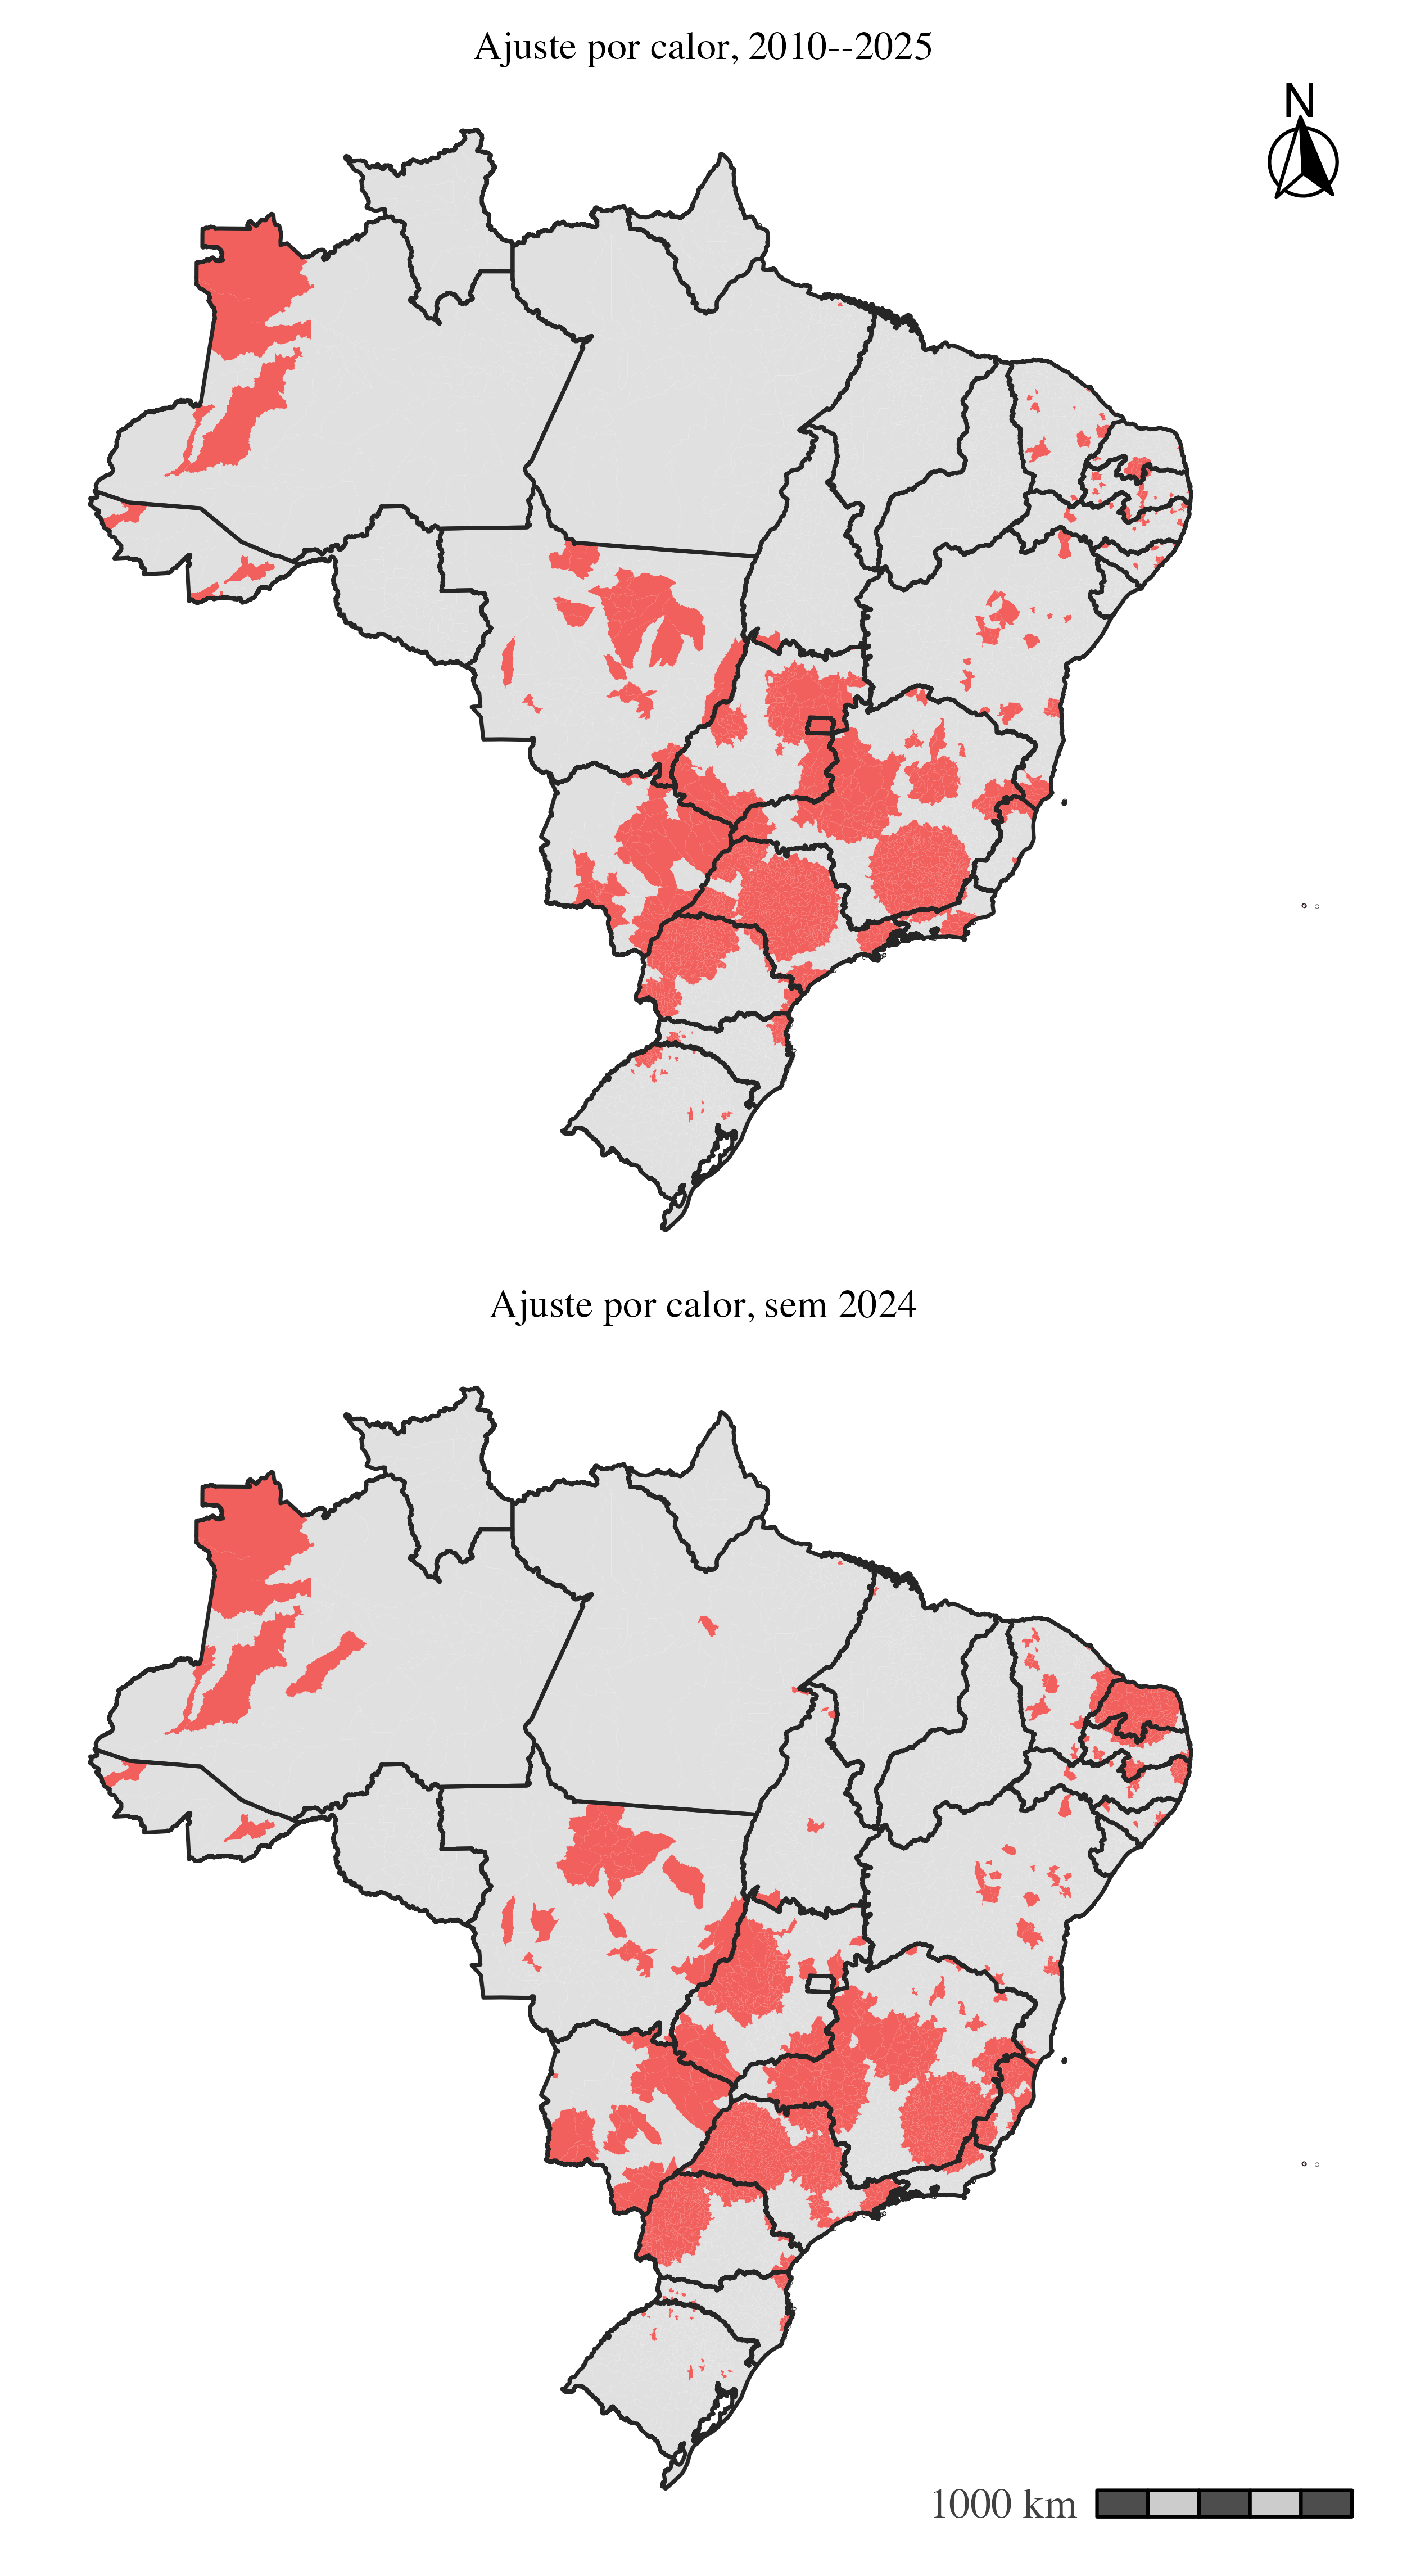
\includegraphics[width=0.66\textwidth]{fig_mapa_clusters_2x1_calor_com_sem2024.png}
    \caption{Zonas de alta incidência sob ajuste por calor com os casos de 2024 (a) e sem os casos de 2024 (b), Brasil. Fontes: SINAN e IBGE.}
    \label{fig:zonas_calor_2024}
    \vspace{0.3em}
    {\footnotesize\noindent\textit{Nota:} Mesma codificação de cor e mesma configuração espacial nos dois painéis; a comparação isola o efeito do período, mantida a padronização pelos tercis de calor.\par}
\end{figure}


\chapter{Discussão e Conclusões}
\label{cap:discussao}

\section{Discussão}
\label{sec:discussao}

Os \ScanTotalCasos{} casos do painel entre 2010 e 2025 apresentam distribuição espacial estruturada e autocorrelação positiva da taxa anual em todos os anos, com valor máximo de Moran em 2024. A elevação das incidências no Sul a partir da segunda metade do período é compatível com a mudança da barreira climática descrita para a região por \citeonline{lee2021}, que também analisaram a relação entre risco de dengue, urbanização e conectividade no Brasil.

A comparação central do trabalho é a varredura espacial com e sem padronização indireta por variáveis térmicas, sanitárias e urbanas, como exercício exploratório. O modelo sem ajuste delimita zonas de excesso sob o limite de 16\% e 200~km; zonas que permanecem ou mudam após cada ajuste indicam heterogeneidade residual, sem demonstrar causalidade \cite{jung2009glm}. O risco acima do esperado segue a formulação de varredura espacial \cite{kulldorff1997spatial}.

Na comparação entre as oito formulações, a coleção passou de 129 zonas sem ajuste para 128 no ajuste por calor, 178 no esgoto adequado, 136 na densidade urbana, 158 na proporção urbana, 193 na água, 195 no lixo e 184 no índice composto. O primário deslocou-se de Adolfo (SP, $RR = 2{,}99$) para Queluzito (MG, $RR = 2{,}08$) sob o ajuste por calor, para Iacri (SP) sob esgoto, proporção urbana, água e lixo, e para Araújos (MG) sob densidade urbana e índice composto. Todos os primários ficaram no Centro-Sul, e a sobreposição municipal com o modelo sem ajuste variou de 56\% (calor) a 82\% (densidade urbana): o eixo de sobre-risco do Centro-Sul manteve-se nas diferentes covariáveis, ainda que a posição do polo primário varie entre formulações.

O WMAPE sintetiza quanto cada padronização aproxima o esperado do observado no conjunto analisado: os valores caíram de 75,1\% sem ajuste para 64,9\% sob calor, 70,5\% sob água, 71,9\% sob esgoto, 71,9\% sob o índice composto, 72,1\% sob lixo, 74,3\% sob densidade urbana e 74,4\% sob proporção urbana. O cálculo é interno à amostra, de modo que a leitura é descritiva: valores menores apontam qual esquema de estratificação melhor acompanha a variabilidade geográfica basal da dengue, sem indicar capacidade preditiva. Um ajuste que absorvesse todo o excesso aproximaria o esperado do observado e reduziria o WMAPE ao custo de esvaziar a detecção; esse limite não foi atingido, pois todas as formulações mantiveram coleções extensas de zonas residuais, entre 128 e 195 zonas, cobrindo de 1.679 a 2.207 municípios com risco relativo primário acima de 2,0. A leitura conjunta das duas medidas orienta a escolha: o ajuste por calor combina a maior redução do WMAPE (10,2 pontos percentuais) com a manutenção de 128 zonas, ao passo que os ajustes por água, esgoto, lixo e índice composto reduzem o erro em menor grau e preservam polos com risco relativo mais alto, entre 2,58 e 2,86.

A decomposição regional mostra que a redução do WMAPE não é uniforme no território. Sob o ajuste por calor, o indicador cai de forma acentuada no Centro-Oeste (53,4\% para 38,7\%), no Sudeste (57,0\% para 43,7\%) e no Sul (101,9\% para 80,9\%), permanece estável no Nordeste (122,2\%) e aumenta no Norte (183,0\% para 245,9\%). O ajuste por água, por sua vez, reduz o indicador no Norte (183,0\% para 109,8\%) e no Nordeste (122,2\% para 106,8\%), com oscilações pequenas nas demais regiões. Como o WMAPE nacional pondera os casos, ele é dominado pelas regiões de maior volume e pode ocultar contrastes regionais como esses.

Sob o ajuste por calor, o polo primário deslocou-se de Adolfo (SP), no modelo sem ajuste, para Queluzito (MG). O risco relativo reportado foi de 2,99 na zona de Adolfo e de 2,08 na zona de Queluzito, que reuniu 362 municípios, ante 319 na zona primária sem ajuste. Como são zonas distintas, essa diferença não mede uma redução do risco no mesmo conjunto de municípios. A configuração das zonas mudou com a padronização térmica, mas essa comparação não estima quanto do excesso se deve ao calor. O aumento do WMAPE no Norte indica que o esquema acompanha menos de perto a distribuição observada nessa região, onde a incidência é mais baixa e a exposição ao calor é alta.

Zonas como Goiânia ($RR = 2{,}40$) e focos no interior de São Paulo, no Paraná e em Santa Catarina sob o modelo ajustado indicam heterogeneidade residual \cite{lee2021}. Fatores sociodemográficos, conectividade e saneamento são hipóteses plausíveis \cite{power2022,cardim2025}, mas não foram estimados neste estudo. A persistência territorial de dez ou mais anos acima de 300 por 100 mil não implica transmissão contínua na mesma população, pois mobilidade e imunidade podem alterar a composição dos grupos suscetíveis \cite{santos2019persistencia}. Nos estratos de saneamento, as taxas acumuladas foram maiores nos níveis com maior cobertura; para densidade urbana, o maior valor ocorreu no tercil intermediário (Seção~\ref{subsec:resultados_estratificacao}). Essas diferenças descritivas podem refletir a composição urbana e populacional dos grupos e a subnotificação diferencial, mas não estimam efeitos do saneamento ou da densidade.

Ao longo das oito formulações, 1.655 municípios (29,7\%) permanecem em zonas significativas em seis ou mais delas, e 967 em todas, com concentração no Centro-Sul (Figura~\ref{fig:robustez}). A persistência nesse eixo sustenta a leitura de heterogeneidade residual estável no Sul, no Sudeste e no Centro-Oeste, que é onde as coleções mais se sobrepõem entre as formulações.

A sensibilidade à exclusão de 2024 reforça a dependência do período acumulado: sem esse ano, os casos do painel caem para 15.664.546 e o número de zonas aumenta na maioria das formulações, com o polo primário deslocado para o interior de São Paulo em quase todas. A sobreposição municipal entre os cenários ficou entre 51\% e 63\%, e o WMAPE nacional aumentou em todas as formulações, indicando que a distribuição de 2010--2023 e 2025 é menos acompanhada pelo esquema de padronização, baseado em população e estratos fixos, do que a série completa. A reexecução sem o ano epidêmico foi motivada também pela investigação etiológica no estado do Rio de Janeiro, que identificou circulação de Oropouche em amostras de casos suspeitos de dengue no período \cite{costa2025oropouche}; a leitura do ano como dengue exclusiva deve, portanto, ser cautelosa.

\section{Conclusões}
\label{cap:conclusoes}

A taxa anual de incidência apresentou autocorrelação espacial positiva em cada um dos 16 anos, com índices globais de Moran entre 0,215 e 0,613 e máximo em 2024. Na análise acumulada sem ajuste, a varredura identificou 129 zonas sem sobreposição (nível nominal de 5\%), que reuniram 64,1\% dos casos do painel em 34,3\% dos municípios; o polo primário foi Adolfo (SP), com 319 municípios e $RR = 2{,}99$.

Os sete ajustes identificaram de 128 a 195 zonas, com deslocamento do primário (Queluzito sob calor, $RR = 2{,}08$; Iacri sob esgoto, proporção urbana, água e lixo; Araújos sob densidade urbana e índice composto). O ajuste por calor combinou a maior redução do erro absoluto percentual ponderado (de 75,1\% para 64,9\%) com a manutenção de 128 zonas residuais; os demais ajustes reduziram o erro entre 0,6 e 4,6 pontos percentuais. Essas comparações são exploratórias.

A reexecução sem 2024 mudou o número de zonas em todas as formulações e a posição do polo primário em sete delas, com sobreposição municipal entre os cenários de 51\% a 63\% e erro absoluto percentual ponderado maior em todos os casos, indicando dependência do período acumulado. A persistência de zonas de alta taxa no Sudeste, no Centro-Oeste e no Sul após as estratificações indica heterogeneidade residual, cuja atribuição a vulnerabilidades estruturais exige análise específica.

Adicionalmente, a sazonalidade e a distribuição regional informam o calendário das ações de vigilância \cite{pescarini2022}.

\section{Limitações e perspectivas}

Há limitações operacionais. Em primeiro lugar, a unidade de agregação ecológica municipal impede capturar a heterogeneidade intraurbana e as ilhas de calor intramunicipais, uma vez que a resolução do ERA5-Land ($\approx 9$~km) atenua contrastes de microescala em grandes metrópoles \cite{rodrigues2018}. Além disso, $T_{\text{máx}}$ é o máximo de quatro instantâneos diários, não o máximo horário contínuo. Em segundo lugar, os dados do SINAN estão sujeitos a atrasos de inserção e subnotificação diferencial; estudos de soroprevalência mostram que notificações sintomáticas podem subestimar substancialmente o número real de infectados \cite{perisse2020soroprevalencia}. Como limites de cobertura, 1.229 casos notificados em Fernando de Noronha, 121 casos em 39 códigos sem correspondência na malha de 2010 e 1.873 casos em 16 registros sem código municipal ficaram fora do painel espacial. Assim, as zonas identificadas devem ser interpretadas como contrastes relativos de notificações. O reporte hierárquico sem correção de multiplicidade torna os resultados exploratórios. Além disso, a varredura acumulada é influenciada pelo ano epidêmico de 2024, que responde por 29,1\% dos casos do painel; a reexecução sem esse ano alterou o número de zonas e os polos primários em sete das oito formulações, como descrito nos Resultados, e parte da coleção corresponde a excessos marginais, cuja significância reflete o volume acumulado sob o modelo de Poisson. A contagem de robustez entre as formulações atribui o mesmo peso a cada uma delas e não pondera a intensidade das zonas, de modo que um município pode manter-se em várias formulações por excessos marginais. Por fim, a janela circular da varredura, ainda que contida pelo teto duplo de 16\% da população e 200~km de raio, impõe restrições geométricas às zonas detectadas; estatísticas flexíveis podem representar melhor formas irregulares, embora também tenham limitações computacionais \cite{tango2005flexible}. Futuros desdobramentos devem incorporar modelos ecológicos explícitos e janelas com formatos flexíveis baseadas, por exemplo, em grafos de transporte.

%%%%%%%%%%%%%%%%%%%%%%%%
%%%INÍCIO DOS APENDICES%
%%%%%%%%%%%%%%%%%%%%%%%%

\apendice
\renewcommand\thechapter{\arabic{chapter}}

\chapter{Tabela Completa de \textit{Clusters} Espaciais}
\label{app:clusters}

A tabela apresenta todos os \textit{clusters} significativos da varredura em rodada única com teto duplo. $RR$ é o risco relativo da zona; os casos esperados são calculados sob o modelo de Poisson e a população média municipal do período.

\begingroup\fontsize{9}{11}\selectfont

\begin{xltabular}{\linewidth}{>{\centering\arraybackslash}X>{\centering\arraybackslash}X>{\centering\arraybackslash}X>{\centering\arraybackslash}X>{\centering\arraybackslash}X>{\centering\arraybackslash}X}
\caption{\label{tab:clusters_satscan_puro}\textit{Clusters} espaciais significativos de dengue detectados pela varredura espacial sem ajuste por covariáveis, Brasil, 2010--2025.}\\
\toprule
\textit{Cluster} & Qtd. municípios & Raio (km) & Casos obs. ($C_Z$) & Casos esp. ($E_Z$) & Risco relativo ($RR_Z$)\\
\midrule
\endfirsthead
\caption[]{\textit{Clusters} espaciais significativos de dengue detectados pela varredura espacial sem ajuste por covariáveis, Brasil, 2010--2025. \textit{(continuação)}}\\
\toprule
\textit{Cluster} & Qtd. municípios & Raio (km) & Casos obs. ($C_Z$) & Casos esp. ($E_Z$) & Risco relativo ($RR_Z$)\\
\midrule
\endhead
\midrule
\multicolumn{6}{r@{}}{\textit{(continuação)}}\\
\endfoot
\bottomrule
\endlastfoot
1 & 319 & 197,4 & 2.342.103 & 842.629 & 2,99\\
2 & 229 & 199,8 & 2.588.779 & 1.019.064 & 2,74\\
3 & 122 & 198,1 & 2.259.957 & 948.039 & 2,54\\
4 & 245 & 198,9 & 1.251.256 & 515.650 & 2,51\\
5 & 48 & 66,5 & 977.272 & 462.096 & 2,17\\
\addlinespace
6 & 136 & 129,0 & 382.821 & 176.908 & 2,18\\
7 & 38 & 99,0 & 528.559 & 288.913 & 1,85\\
8 & 8 & 43,5 & 221.354 & 85.286 & 2,61\\
9 & 43 & 165,6 & 196.827 & 76.218 & 2,60\\
10 & 23 & 197,6 & 251.787 & 128.381 & 1,97\\
\addlinespace
11 & 1 & 0,0 & 46.111 & 9.322 & 4,95\\
12 & 134 & 107,1 & 414.194 & 268.589 & 1,55\\
13 & 178 & 198,4 & 438.280 & 300.249 & 1,47\\
14 & 10 & 30,0 & 199.249 & 120.188 & 1,66\\
15 & 21 & 199,5 & 85.974 & 44.806 & 1,92\\
\addlinespace
16 & 36 & 186,0 & 117.247 & 68.871 & 1,71\\
17 & 10 & 30,5 & 155.307 & 99.551 & 1,56\\
18 & 61 & 191,0 & 120.223 & 75.308 & 1,60\\
19 & 3 & 58,5 & 78.666 & 44.450 & 1,77\\
20 & 3 & 14,1 & 64.151 & 34.479 & 1,86\\
\addlinespace
21 & 4 & 17,9 & 76.625 & 44.302 & 1,73\\
22 & 1 & 0,0 & 66.301 & 37.511 & 1,77\\
23 & 3 & 74,5 & 22.399 & 7.900 & 2,84\\
24 & 1 & 0,0 & 48.486 & 24.863 & 1,95\\
25 & 22 & 44,6 & 44.577 & 24.704 & 1,81\\
\addlinespace
26 & 3 & 36,6 & 36.003 & 19.051 & 1,89\\
27 & 1 & 0,0 & 124.442 & 90.308 & 1,38\\
28 & 1 & 0,0 & 37.737 & 21.788 & 1,73\\
29 & 1 & 0,0 & 49.428 & 30.782 & 1,61\\
30 & 17 & 147,4 & 87.943 & 64.309 & 1,37\\
\addlinespace
31 & 3 & 10,7 & 10.112 & 4.128 & 2,45\\
32 & 3 & 38,8 & 60.398 & 43.145 & 1,40\\
33 & 11 & 34,0 & 23.602 & 14.423 & 1,64\\
34 & 1 & 0,0 & 10.437 & 5.546 & 1,88\\
35 & 1 & 0,0 & 7.958 & 3.860 & 2,06\\
\addlinespace
36 & 1 & 0,0 & 9.754 & 5.296 & 1,84\\
37 & 9 & 32,7 & 13.904 & 8.844 & 1,57\\
38 & 1 & 0,0 & 15.621 & 10.214 & 1,53\\
39 & 13 & 144,7 & 31.514 & 23.650 & 1,33\\
40 & 6 & 142,6 & 15.500 & 10.294 & 1,51\\
\addlinespace
41 & 1 & 0,0 & 32.709 & 24.980 & 1,31\\
42 & 1 & 0,0 & 12.519 & 8.003 & 1,56\\
43 & 1 & 0,0 & 21.847 & 15.867 & 1,38\\
44 & 9 & 50,9 & 26.731 & 20.207 & 1,32\\
45 & 1 & 0,0 & 64.072 & 53.782 & 1,19\\
\addlinespace
46 & 1 & 0,0 & 6.714 & 3.835 & 1,75\\
47 & 3 & 15,3 & 4.319 & 2.117 & 2,04\\
48 & 2 & 18,8 & 6.542 & 3.760 & 1,74\\
49 & 1 & 0,0 & 2.875 & 1.199 & 2,40\\
50 & 1 & 0,0 & 10.723 & 7.039 & 1,52\\
\addlinespace
51 & 3 & 165,0 & 7.386 & 4.433 & 1,67\\
52 & 1 & 0,0 & 7.833 & 4.859 & 1,61\\
53 & 1 & 0,0 & 6.292 & 3.721 & 1,69\\
54 & 1 & 0,0 & 12.350 & 8.791 & 1,41\\
55 & 1 & 0,0 & 14.655 & 10.860 & 1,35\\
\addlinespace
56 & 1 & 0,0 & 5.561 & 3.392 & 1,64\\
57 & 2 & 26,7 & 4.984 & 2.982 & 1,67\\
58 & 3 & 16,9 & 5.483 & 3.419 & 1,60\\
59 & 1 & 0,0 & 2.350 & 1.128 & 2,08\\
60 & 5 & 35,0 & 12.871 & 9.609 & 1,34\\
\addlinespace
61 & 1 & 0,0 & 5.399 & 3.445 & 1,57\\
62 & 3 & 131,6 & 8.807 & 6.240 & 1,41\\
63 & 1 & 0,0 & 5.078 & 3.244 & 1,57\\
64 & 1 & 0,0 & 6.091 & 4.068 & 1,50\\
65 & 4 & 185,8 & 21.462 & 17.525 & 1,22\\
\addlinespace
66 & 1 & 0,0 & 10.515 & 7.872 & 1,34\\
67 & 3 & 108,2 & 11.469 & 8.742 & 1,31\\
68 & 1 & 0,0 & 12.048 & 9.292 & 1,30\\
69 & 1 & 0,0 & 2.211 & 1.172 & 1,89\\
70 & 1 & 0,0 & 8.522 & 6.323 & 1,35\\
\addlinespace
71 & 1 & 0,0 & 8.763 & 6.538 & 1,34\\
72 & 1 & 0,0 & 3.286 & 2.010 & 1,64\\
73 & 1 & 0,0 & 2.679 & 1.598 & 1,68\\
74 & 1 & 0,0 & 6.072 & 4.361 & 1,39\\
75 & 1 & 0,0 & 733 & 291 & 2,52\\
\addlinespace
76 & 1 & 0,0 & 2.514 & 1.603 & 1,57\\
77 & 1 & 0,0 & 4.585 & 3.309 & 1,39\\
78 & 3 & 99,8 & 5.520 & 4.171 & 1,32\\
79 & 1 & 0,0 & 2.848 & 1.954 & 1,46\\
80 & 1 & 0,0 & 10.807 & 8.972 & 1,20\\
\addlinespace
81 & 1 & 0,0 & 3.609 & 2.629 & 1,37\\
82 & 1 & 0,0 & 952 & 500 & 1,90\\
83 & 1 & 0,0 & 3.347 & 2.418 & 1,38\\
84 & 1 & 0,0 & 2.690 & 1.901 & 1,41\\
85 & 1 & 0,0 & 1.932 & 1.300 & 1,49\\
\addlinespace
86 & 1 & 0,0 & 7.733 & 6.387 & 1,21\\
87 & 5 & 63,8 & 11.486 & 9.883 & 1,16\\
88 & 2 & 11,9 & 63.457 & 59.585 & 1,07\\
89 & 1 & 0,0 & 2.955 & 2.210 & 1,34\\
90 & 1 & 0,0 & 3.571 & 2.767 & 1,29\\
\addlinespace
91 & 1 & 0,0 & 2.730 & 2.038 & 1,34\\
92 & 1 & 0,0 & 28.593 & 26.204 & 1,09\\
93 & 1 & 0,0 & 2.820 & 2.125 & 1,33\\
94 & 1 & 0,0 & 9.917 & 8.577 & 1,16\\
95 & 1 & 0,0 & 2.233 & 1.641 & 1,36\\
\addlinespace
96 & 5 & 24,8 & 10.747 & 9.437 & 1,14\\
97 & 1 & 0,0 & 847 & 528 & 1,60\\
98 & 1 & 0,0 & 3.901 & 3.166 & 1,23\\
99 & 1 & 0,0 & 1.424 & 1.000 & 1,42\\
100 & 1 & 0,0 & 1.067 & 719 & 1,48\\
\addlinespace
101 & 2 & 22,6 & 7.997 & 6.964 & 1,15\\
102 & 1 & 0,0 & 2.346 & 1.818 & 1,29\\
103 & 1 & 0,0 & 2.558 & 2.021 & 1,27\\
104 & 1 & 0,0 & 912 & 610 & 1,50\\
105 & 1 & 0,0 & 1.018 & 703 & 1,45\\
\addlinespace
106 & 1 & 0,0 & 783 & 515 & 1,52\\
107 & 5 & 20,4 & 12.755 & 11.583 & 1,10\\
108 & 2 & 30,9 & 2.562 & 2.072 & 1,24\\
109 & 1 & 0,0 & 2.585 & 2.097 & 1,23\\
110 & 1 & 0,0 & 2.598 & 2.124 & 1,22\\
\addlinespace
111 & 1 & 0,0 & 449 & 274 & 1,64\\
112 & 1 & 0,0 & 1.417 & 1.087 & 1,30\\
113 & 1 & 0,0 & 1.122 & 857 & 1,31\\
114 & 1 & 0,0 & 710 & 511 & 1,39\\
115 & 1 & 0,0 & 928 & 700 & 1,33\\
\addlinespace
116 & 1 & 0,0 & 17.764 & 16.711 & 1,06\\
117 & 1 & 0,0 & 6.339 & 5.731 & 1,11\\
118 & 1 & 0,0 & 462 & 323 & 1,43\\
119 & 4 & 14,2 & 2.039 & 1.734 & 1,18\\
120 & 1 & 0,0 & 862 & 673 & 1,28\\
\addlinespace
121 & 1 & 0,0 & 407 & 284 & 1,43\\
122 & 1 & 0,0 & 2.218 & 1.935 & 1,15\\
123 & 1 & 0,0 & 800 & 639 & 1,25\\
124 & 1 & 0,0 & 802 & 645 & 1,24\\
125 & 1 & 0,0 & 1.420 & 1.210 & 1,17\\
\addlinespace
126 & 1 & 0,0 & 2.587 & 2.301 & 1,12\\
127 & 1 & 0,0 & 598 & 471 & 1,27\\
128 & 1 & 0,0 & 9.754 & 9.214 & 1,06\\
129 & 1 & 0,0 & 1.802 & 1.599 & 1,13\\*
\end{xltabular}
\endgroup{}


\par\vspace{0.4em}
\parbox{\linewidth}{\footnotesize\textit{Nota:} A tabela não apresenta município polo; a ordenação segue a coleção reportada pelo programa. Valores de casos e risco relativo são os estimados para 2010--2025.}

\chapter{Tabela Completa de \textit{Clusters} com Ajuste Térmico}
\label{app:clusters_termica}

A tabela apresenta as zonas da varredura em rodada única com padronização indireta pelos tercis de dias sob onda de calor. Os valores devem ser interpretados como resultado exploratório da análise ajustada, não como estimativas de efeito causal da temperatura.

\begingroup\fontsize{9}{11}\selectfont

\begin{xltabular}{\linewidth}{>{\centering\arraybackslash}X>{\centering\arraybackslash}X>{\centering\arraybackslash}X>{\centering\arraybackslash}X>{\centering\arraybackslash}X>{\centering\arraybackslash}X}
\caption{\label{tab:clusters_satscan_termica}\textit{Clusters} espaciais significativos de dengue detectados pela varredura espacial sob padronização indireta pelos tercis de dias em onda de calor, Brasil, 2010--2025.}\\
\toprule
\textit{Cluster} & Qtd. municípios & Raio (km) & Casos obs. ($C_Z$) & Casos esp. ($E_Z$) & Risco relativo ($RR_Z$)\\
\midrule
\endfirsthead
\caption[]{\textit{Clusters} espaciais significativos de dengue detectados pela varredura espacial sob padronização indireta pelos tercis de dias em onda de calor, Brasil, 2010--2025. \textit{(continuação)}}\\
\toprule
\textit{Cluster} & Qtd. municípios & Raio (km) & Casos obs. ($C_Z$) & Casos esp. ($E_Z$) & Risco relativo ($RR_Z$)\\
\midrule
\endhead
\midrule
\multicolumn{6}{r@{}}{\textit{(continuação)}}\\
\endfoot
\bottomrule
\endlastfoot
1 & 362 & 199,5 & 2.967.585 & 1.533.663 & 2,08\\
2 & 335 & 199,3 & 3.232.573 & 1.868.613 & 1,86\\
3 & 3 & 18,8 & 810.059 & 344.386 & 2,40\\
4 & 245 & 198,9 & 1.267.677 & 663.178 & 1,97\\
5 & 38 & 99,0 & 528.559 & 185.110 & 2,90\\
\addlinespace
6 & 26 & 70,8 & 408.413 & 146.361 & 2,82\\
7 & 45 & 82,8 & 368.333 & 160.010 & 2,32\\
8 & 105 & 197,5 & 461.706 & 270.945 & 1,72\\
9 & 1 & 0,0 & 46.111 & 10.214 & 4,52\\
10 & 2 & 121,0 & 130.373 & 58.493 & 2,24\\
\addlinespace
11 & 9 & 41,3 & 87.296 & 33.935 & 2,58\\
12 & 2 & 14,3 & 128.239 & 60.392 & 2,13\\
13 & 75 & 198,8 & 531.276 & 380.155 & 1,41\\
14 & 1 & 0,0 & 48.486 & 15.930 & 3,05\\
15 & 15 & 83,1 & 67.798 & 28.962 & 2,35\\
\addlinespace
16 & 58 & 166,2 & 1.011.751 & 853.839 & 1,19\\
17 & 3 & 38,8 & 60.398 & 28.517 & 2,12\\
18 & 24 & 73,4 & 69.719 & 36.928 & 1,89\\
19 & 20 & 49,1 & 38.268 & 18.156 & 2,11\\
20 & 23 & 81,8 & 175.388 & 131.149 & 1,34\\
\addlinespace
21 & 33 & 57,7 & 57.425 & 34.354 & 1,67\\
22 & 3 & 10,7 & 10.112 & 2.645 & 3,82\\
23 & 1 & 0,0 & 225.675 & 178.132 & 1,27\\
24 & 6 & 19,3 & 109.745 & 79.792 & 1,38\\
25 & 11 & 125,9 & 214.584 & 172.820 & 1,24\\
\addlinespace
26 & 10 & 105,0 & 40.851 & 24.267 & 1,68\\
27 & 8 & 15,9 & 55.731 & 36.793 & 1,52\\
28 & 24 & 101,0 & 65.264 & 44.734 & 1,46\\
29 & 1 & 0,0 & 76.901 & 55.764 & 1,38\\
30 & 1 & 0,0 & 12.350 & 5.632 & 2,19\\
\addlinespace
31 & 3 & 74,5 & 22.399 & 12.764 & 1,76\\
32 & 3 & 18,8 & 7.000 & 2.643 & 2,65\\
33 & 5 & 15,1 & 17.944 & 10.716 & 1,67\\
34 & 13 & 93,9 & 26.549 & 17.986 & 1,48\\
35 & 14 & 83,7 & 41.877 & 30.847 & 1,36\\
\addlinespace
36 & 2 & 26,7 & 4.984 & 1.911 & 2,61\\
37 & 1 & 0,0 & 6.091 & 2.607 & 2,34\\
38 & 1 & 0,0 & 5.399 & 2.207 & 2,45\\
39 & 13 & 180,0 & 58.224 & 45.575 & 1,28\\
40 & 2 & 37,1 & 13.503 & 8.303 & 1,63\\
\addlinespace
41 & 8 & 100,7 & 35.309 & 26.444 & 1,34\\
42 & 1 & 0,0 & 9.754 & 5.803 & 1,68\\
43 & 3 & 21,8 & 11.986 & 7.657 & 1,57\\
44 & 1 & 0,0 & 3.722 & 1.639 & 2,27\\
45 & 1 & 0,0 & 3.024 & 1.259 & 2,40\\
\addlinespace
46 & 2 & 56,0 & 6.258 & 3.554 & 1,76\\
47 & 1 & 0,0 & 2.514 & 1.027 & 2,45\\
48 & 2 & 12,2 & 8.054 & 5.114 & 1,58\\
49 & 14 & 26,2 & 19.990 & 15.135 & 1,32\\
50 & 1 & 0,0 & 2.955 & 1.416 & 2,09\\
\addlinespace
51 & 1 & 0,0 & 2.730 & 1.306 & 2,09\\
52 & 4 & 35,2 & 14.209 & 10.570 & 1,34\\
53 & 4 & 20,5 & 3.322 & 1.745 & 1,90\\
54 & 1 & 0,0 & 10.723 & 7.713 & 1,39\\
55 & 2 & 20,6 & 7.618 & 5.158 & 1,48\\
\addlinespace
56 & 1 & 0,0 & 2.233 & 1.052 & 2,12\\
57 & 2 & 15,5 & 22.419 & 18.095 & 1,24\\
58 & 1 & 0,0 & 2.558 & 1.295 & 1,98\\
59 & 1 & 0,0 & 2.585 & 1.344 & 1,92\\
60 & 3 & 74,7 & 16.175 & 12.662 & 1,28\\
\addlinespace
61 & 1 & 0,0 & 2.378 & 1.206 & 1,97\\
62 & 1 & 0,0 & 2.774 & 1.571 & 1,77\\
63 & 1 & 0,0 & 72.558 & 65.610 & 1,11\\
64 & 1 & 0,0 & 1.424 & 641 & 2,22\\
65 & 1 & 0,0 & 2.827 & 1.668 & 1,70\\
\addlinespace
66 & 1 & 0,0 & 4.700 & 3.161 & 1,49\\
67 & 1 & 0,0 & 2.180 & 1.220 & 1,79\\
68 & 2 & 27,0 & 2.552 & 1.561 & 1,63\\
69 & 2 & 14,9 & 16.311 & 13.588 & 1,20\\
70 & 1 & 0,0 & 3.286 & 2.202 & 1,49\\
\addlinespace
71 & 1 & 0,0 & 10.515 & 8.625 & 1,22\\
72 & 1 & 0,0 & 8.522 & 6.928 & 1,23\\
73 & 1 & 0,0 & 8.763 & 7.163 & 1,22\\
74 & 1 & 0,0 & 800 & 409 & 1,95\\
75 & 1 & 0,0 & 4.360 & 3.331 & 1,31\\
\addlinespace
76 & 1 & 0,0 & 1.274 & 767 & 1,66\\
77 & 1 & 0,0 & 952 & 548 & 1,74\\
78 & 1 & 0,0 & 951 & 549 & 1,73\\
79 & 1 & 0,0 & 10.351 & 8.868 & 1,17\\
80 & 1 & 0,0 & 5.459 & 4.407 & 1,24\\
\addlinespace
81 & 1 & 0,0 & 10.437 & 8.961 & 1,16\\
82 & 1 & 0,0 & 2.070 & 1.496 & 1,38\\
83 & 1 & 0,0 & 1.476 & 1.006 & 1,47\\
84 & 1 & 0,0 & 6.332 & 5.301 & 1,19\\
85 & 1 & 0,0 & 1.837 & 1.312 & 1,40\\
\addlinespace
86 & 1 & 0,0 & 1.141 & 752 & 1,52\\
87 & 1 & 0,0 & 3.609 & 2.881 & 1,25\\
88 & 1 & 0,0 & 3.347 & 2.650 & 1,26\\
89 & 1 & 0,0 & 1.849 & 1.377 & 1,34\\
90 & 1 & 0,0 & 525 & 296 & 1,77\\
\addlinespace
91 & 1 & 0,0 & 3.270 & 2.632 & 1,24\\
92 & 3 & 38,0 & 10.512 & 9.346 & 1,12\\
93 & 1 & 0,0 & 565 & 334 & 1,69\\
94 & 1 & 0,0 & 2.819 & 2.262 & 1,25\\
95 & 1 & 0,0 & 687 & 439 & 1,57\\
\addlinespace
96 & 3 & 18,5 & 6.536 & 5.746 & 1,14\\
97 & 1 & 0,0 & 2.106 & 1.678 & 1,26\\
98 & 2 & 19,9 & 3.308 & 2.771 & 1,19\\
99 & 1 & 0,0 & 658 & 437 & 1,51\\
100 & 1 & 0,0 & 10.807 & 9.830 & 1,10\\
\addlinespace
101 & 1 & 0,0 & 1.067 & 787 & 1,36\\
102 & 1 & 0,0 & 1.295 & 985 & 1,32\\
103 & 1 & 0,0 & 681 & 466 & 1,46\\
104 & 1 & 0,0 & 1.148 & 862 & 1,33\\
105 & 2 & 27,7 & 2.410 & 1.989 & 1,21\\
\addlinespace
106 & 1 & 0,0 & 3.201 & 2.721 & 1,18\\
107 & 1 & 0,0 & 373 & 229 & 1,63\\
108 & 1 & 0,0 & 439 & 281 & 1,56\\
109 & 1 & 0,0 & 1.884 & 1.532 & 1,23\\
110 & 1 & 0,0 & 1.049 & 795 & 1,32\\
\addlinespace
111 & 1 & 0,0 & 1.018 & 770 & 1,32\\
112 & 1 & 0,0 & 502 & 339 & 1,48\\
113 & 1 & 0,0 & 625 & 443 & 1,41\\
114 & 1 & 0,0 & 2.625 & 2.242 & 1,17\\
115 & 1 & 0,0 & 869 & 664 & 1,31\\
\addlinespace
116 & 1 & 0,0 & 1.167 & 928 & 1,26\\
117 & 1 & 0,0 & 2.211 & 1.893 & 1,17\\
118 & 1 & 0,0 & 1.608 & 1.349 & 1,19\\
119 & 1 & 0,0 & 2.226 & 1.924 & 1,16\\
120 & 2 & 34,8 & 7.542 & 6.977 & 1,08\\
\addlinespace
121 & 1 & 0,0 & 6.714 & 6.196 & 1,08\\
122 & 1 & 0,0 & 1.417 & 1.191 & 1,19\\
123 & 2 & 45,5 & 2.380 & 2.095 & 1,14\\
124 & 1 & 0,0 & 288 & 200 & 1,44\\
125 & 1 & 0,0 & 1.122 & 938 & 1,20\\
\addlinespace
126 & 1 & 0,0 & 928 & 767 & 1,21\\
127 & 1 & 0,0 & 3.627 & 3.337 & 1,09\\
128 & 1 & 0,0 & 1.141 & 984 & 1,16\\*
\end{xltabular}
\endgroup{}


\par\vspace{0.4em}
\parbox{\linewidth}{\footnotesize\textit{Nota:} A tabela não apresenta município polo; a ordenação segue a coleção reportada pelo programa. Valores de casos, expectativa e risco relativo são os estimados para 2010--2025.}

\chapter{Pranchas de zonas e de risco relativo}
\label{app:pranchas}

As pranchas reúnem, em uma página cada, os oito mapas de zonas significativas de 2010--2025 (Figura~\ref{fig:prancha_clusters}), os oito do cenário sem 2024 (Figura~\ref{fig:prancha_clusters_sem2024}) e os seis mapas de risco relativo das demais formulações (Figura~\ref{fig:prancha_rr}). O desenho é compacto: uma escala gráfica e uma rosa dos ventos por prancha, painéis em ordem de leitura e sem contorno municipal individual. A leitura município a município deve usar as figuras do corpo e as tabelas de \textit{clusters} dos Apêndices~\ref{app:clusters} e \ref{app:clusters_termica}.

\begin{figure}[H]
    \centering
    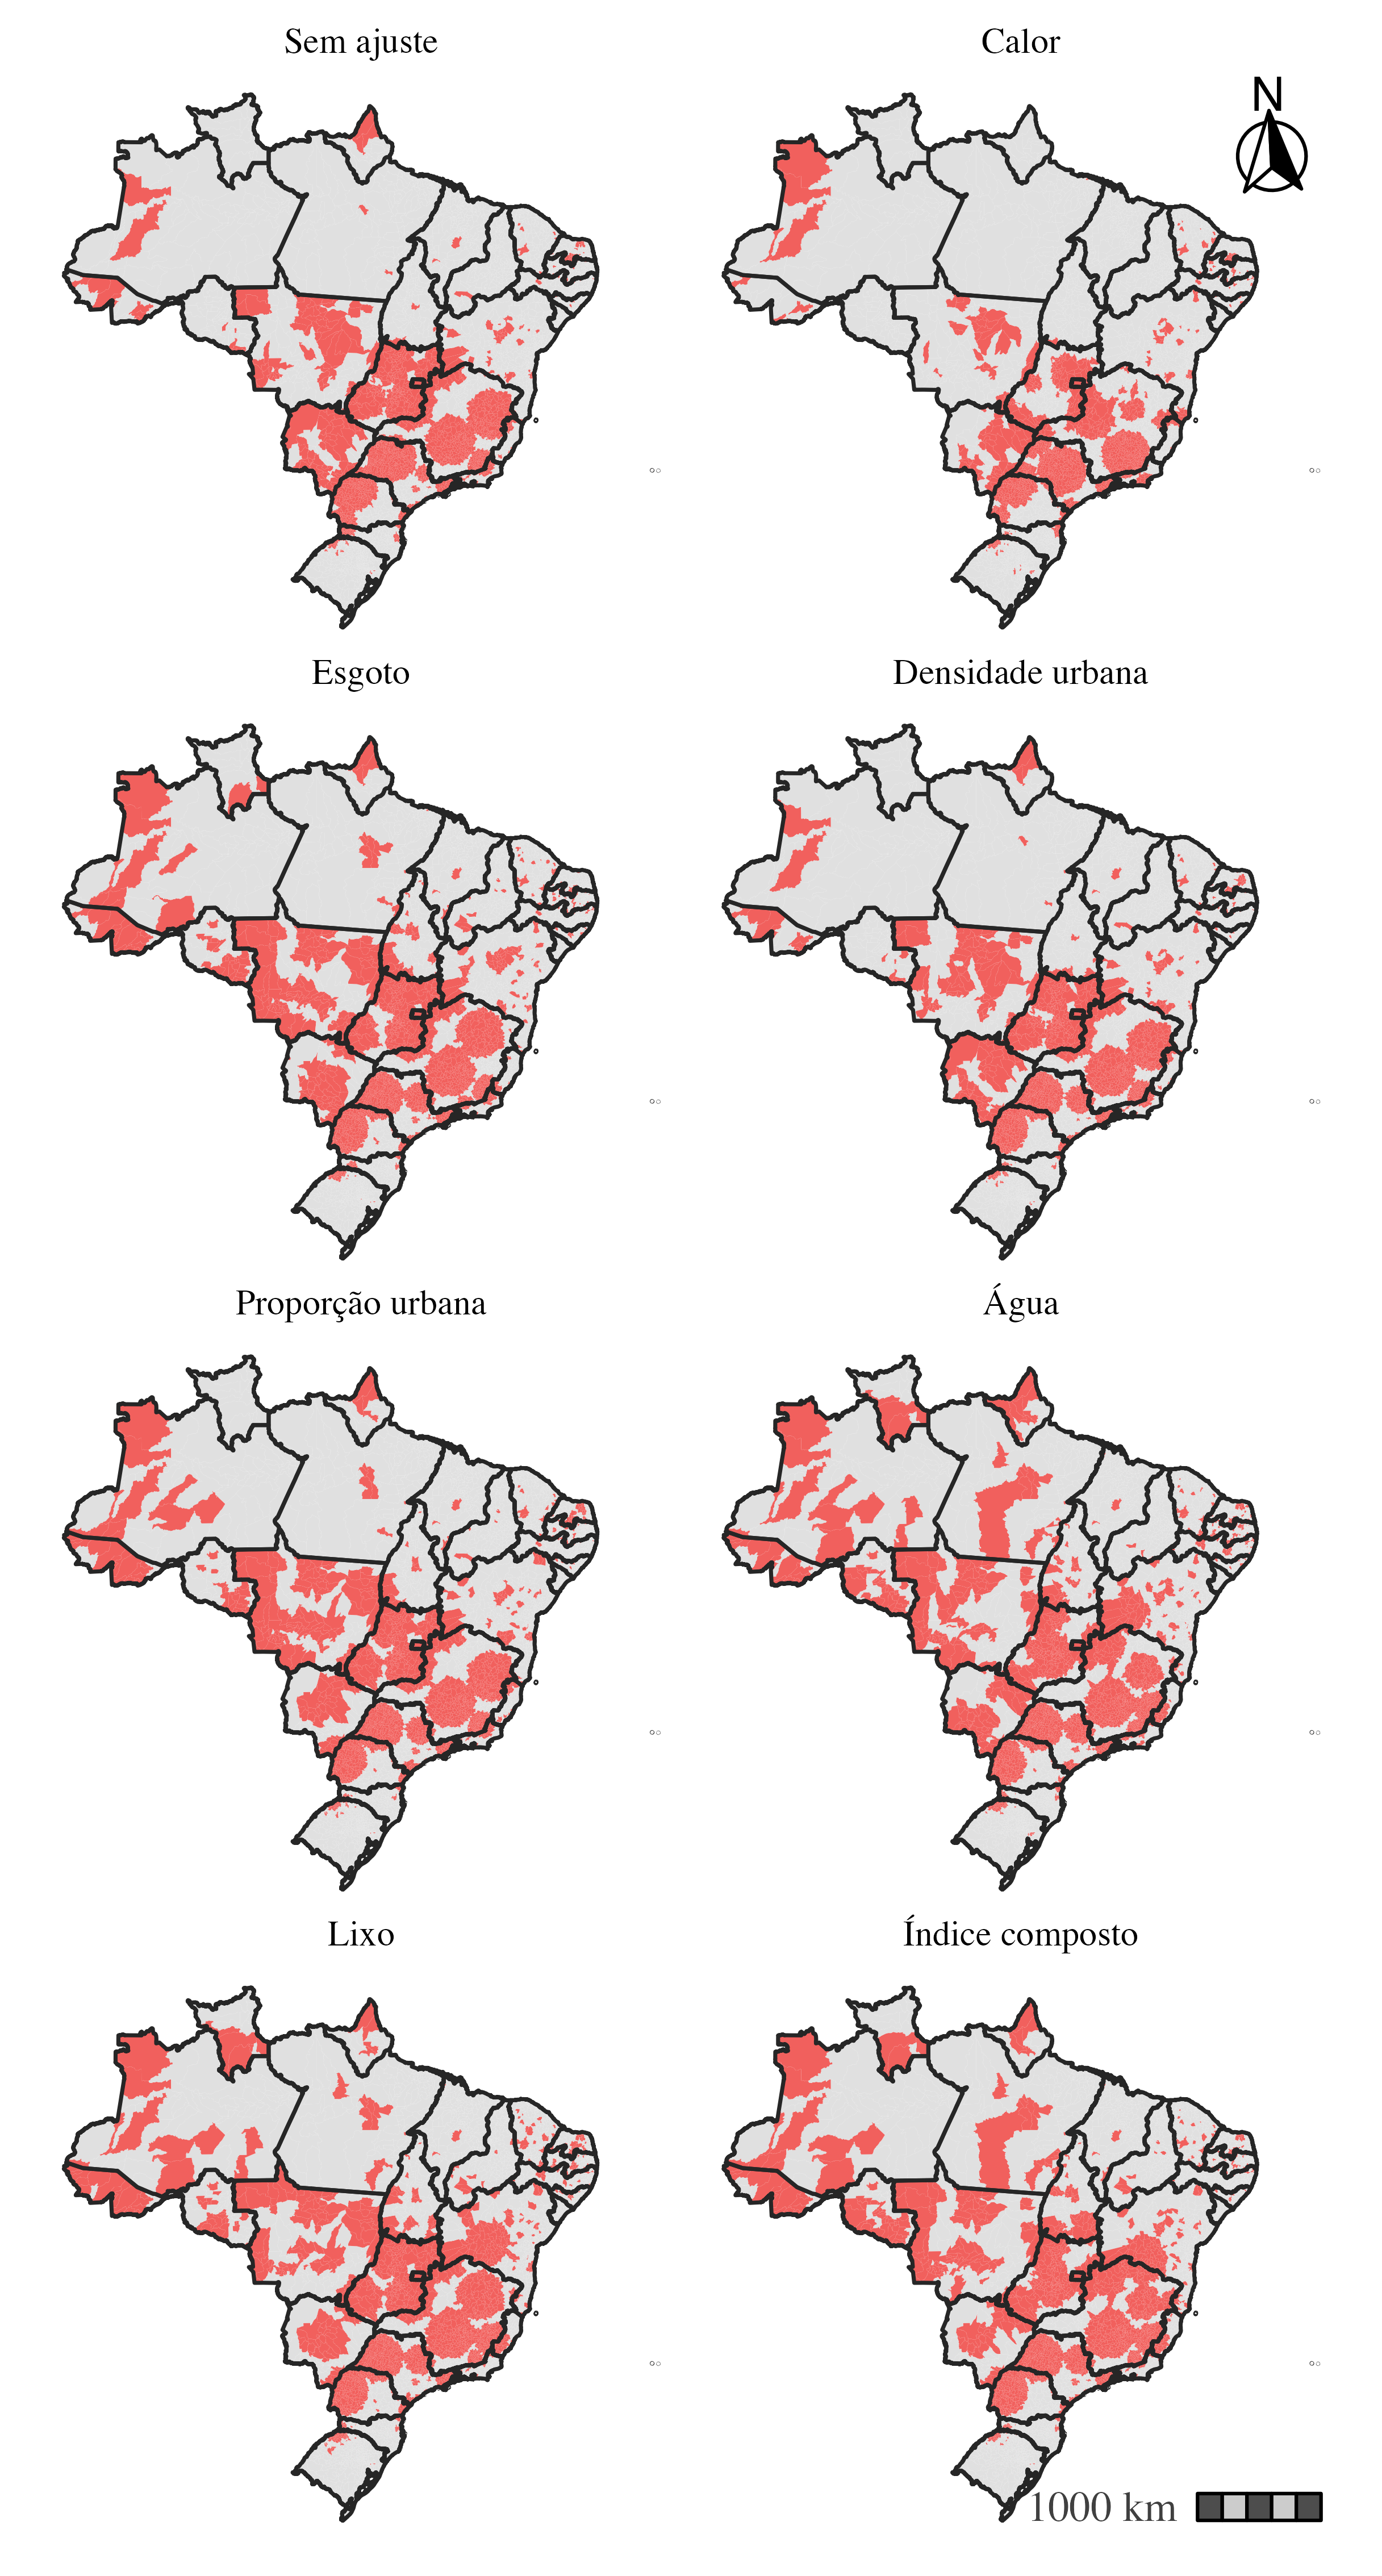
\includegraphics[width=0.60\textwidth]{fig_prancha_clusters_completo.png}
    \caption{Zonas significativas de alto risco por formulação da varredura espacial, Brasil, 2010--2025, em ordem de leitura: sem ajuste, calor, esgoto, densidade urbana, proporção urbana, água, lixo e índice composto. Fontes: SINAN e IBGE.}
    \label{fig:prancha_clusters}
    \vspace{0.3em}
    {\footnotesize\noindent\textit{Nota:} Em laranja, municípios em zonas com nível de 5\%; em cinza, municípios fora de zonas. Todas as formulações usam o mesmo limite de 16\% da população e 200~km, com 999 réplicas e reporte sem sobreposição geográfica.\par}
\end{figure}

\begin{figure}[H]
    \centering
    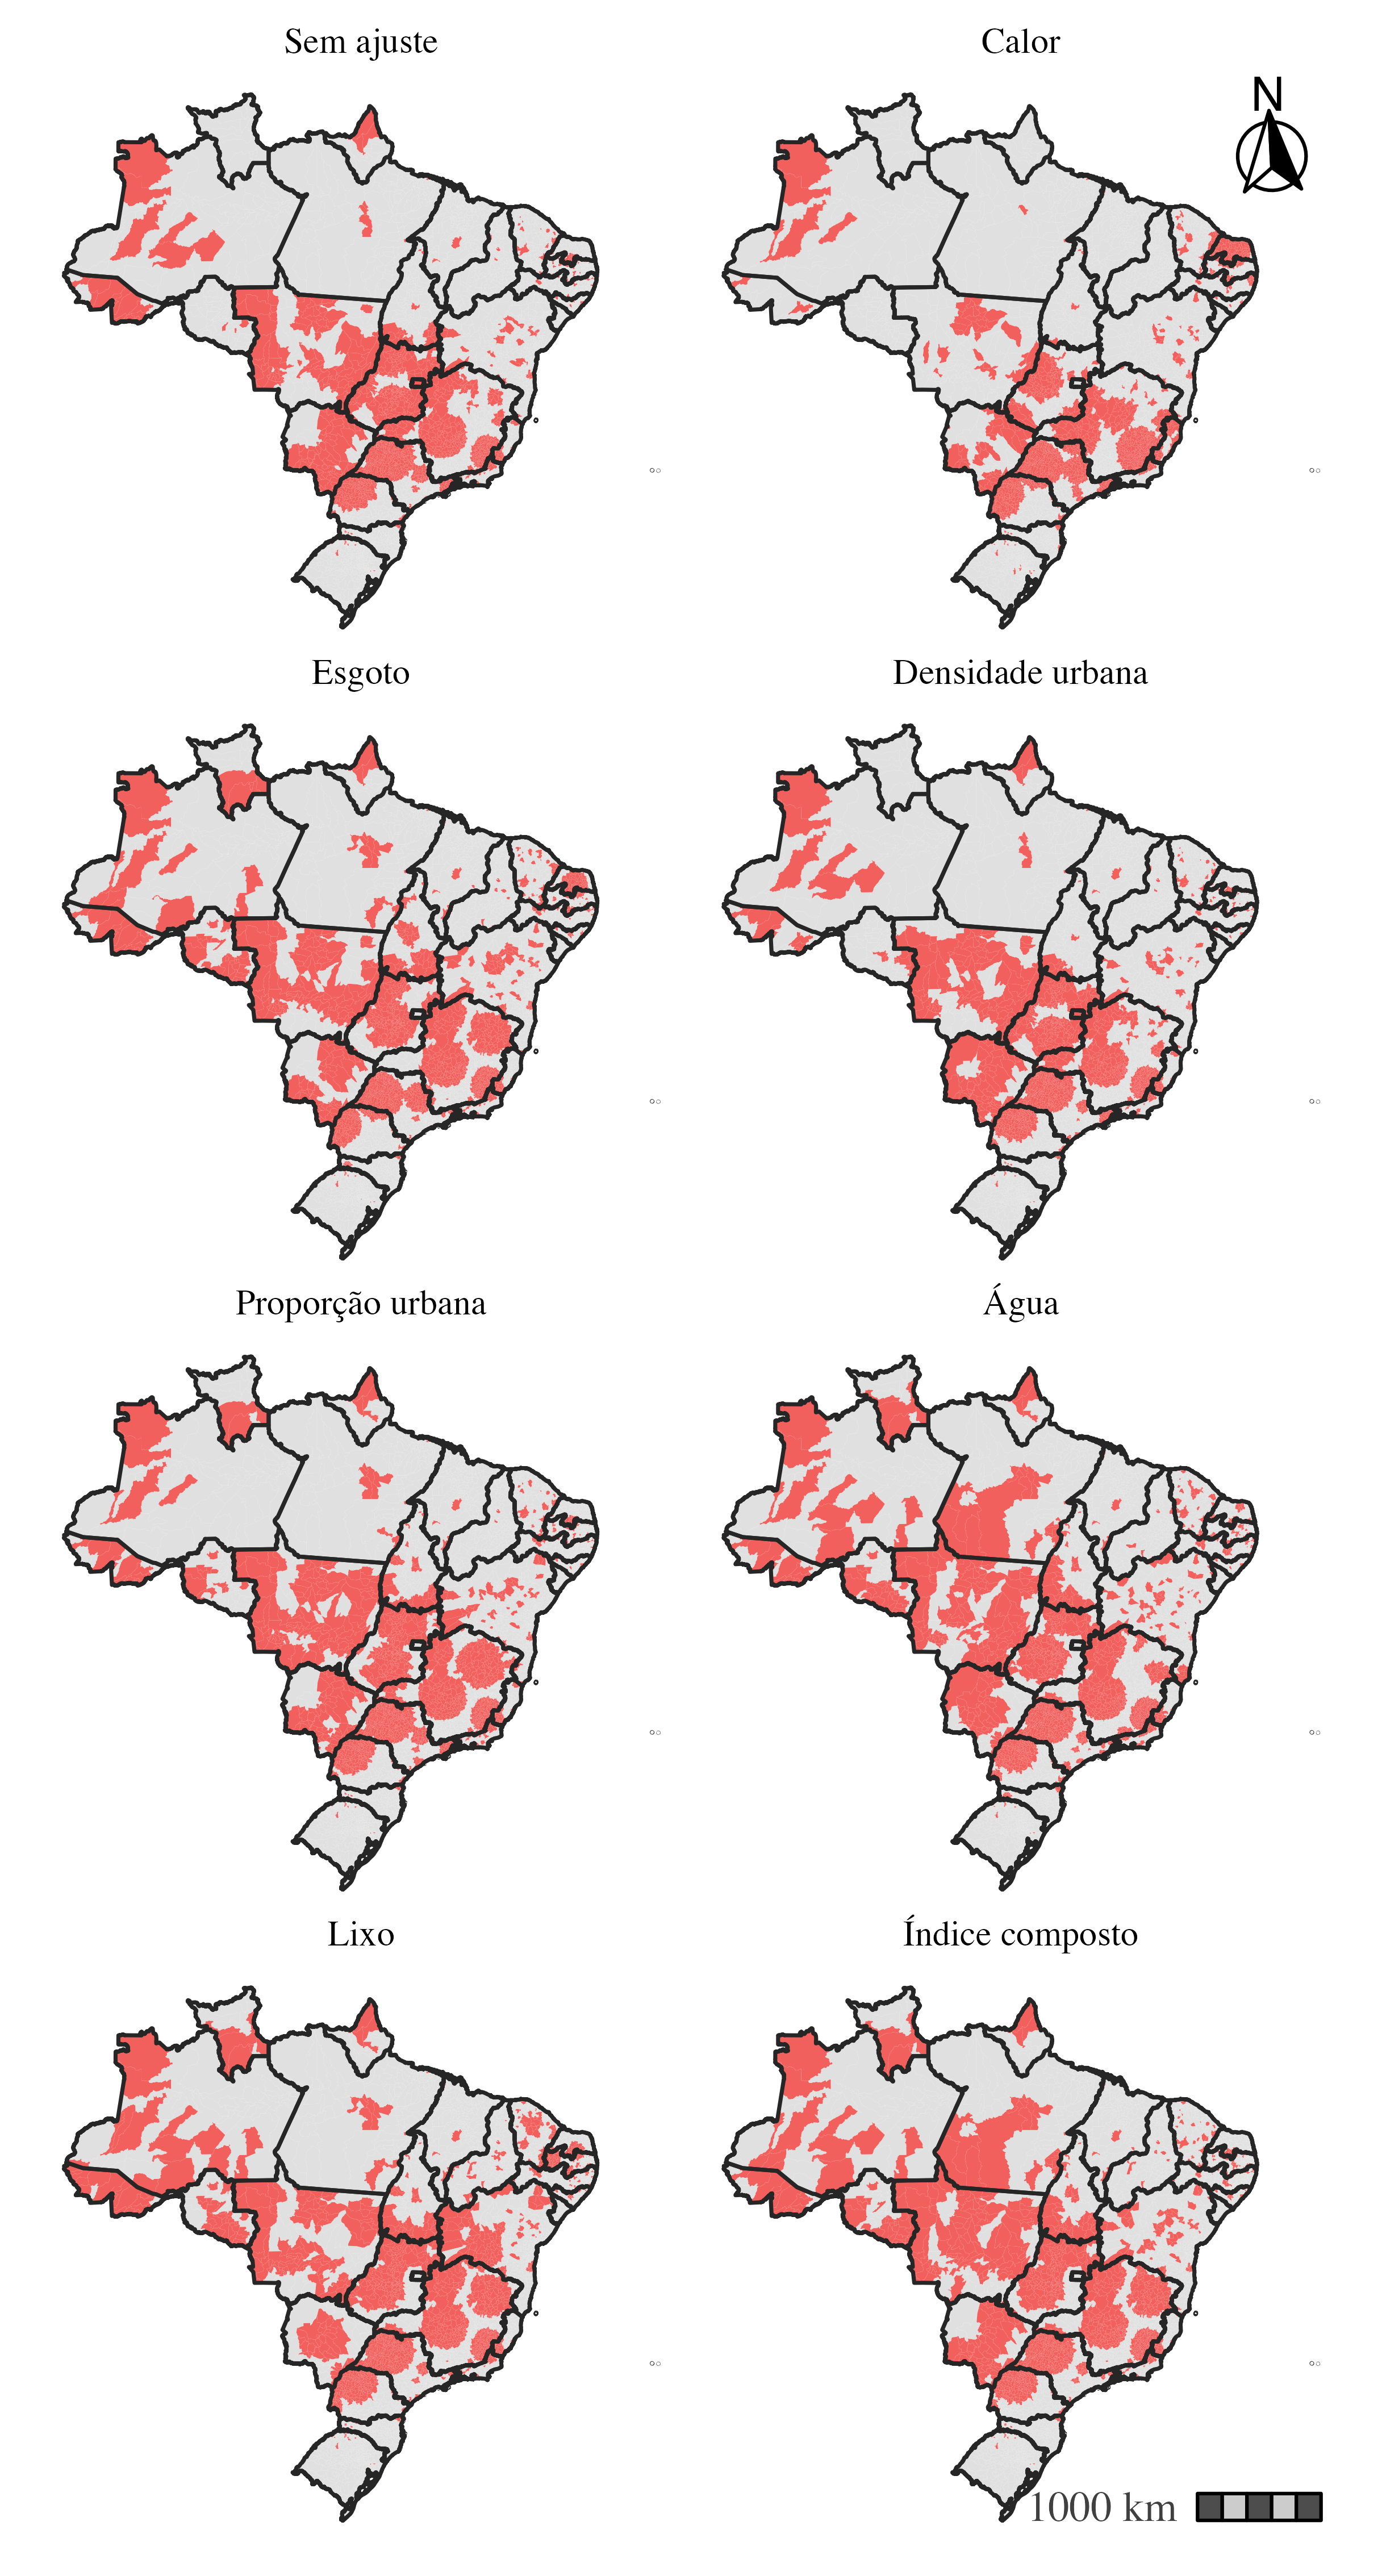
\includegraphics[width=0.60\textwidth]{fig_prancha_clusters_sem2024.png}
    \caption{Zonas significativas de alto risco por formulação da varredura espacial sem os casos de 2024, Brasil, 2010--2023 e 2025, em ordem de leitura: sem ajuste, calor, esgoto, densidade urbana, proporção urbana, água, lixo e índice composto. Fontes: SINAN e IBGE.}
    \label{fig:prancha_clusters_sem2024}
    \vspace{0.3em}
    {\footnotesize\noindent\textit{Nota:} Mesma codificação de cor e mesma configuração da prancha anterior; o painel sem 2024 reúne 15.664.546 casos.\par}
\end{figure}

\begin{figure}[H]
    \centering
    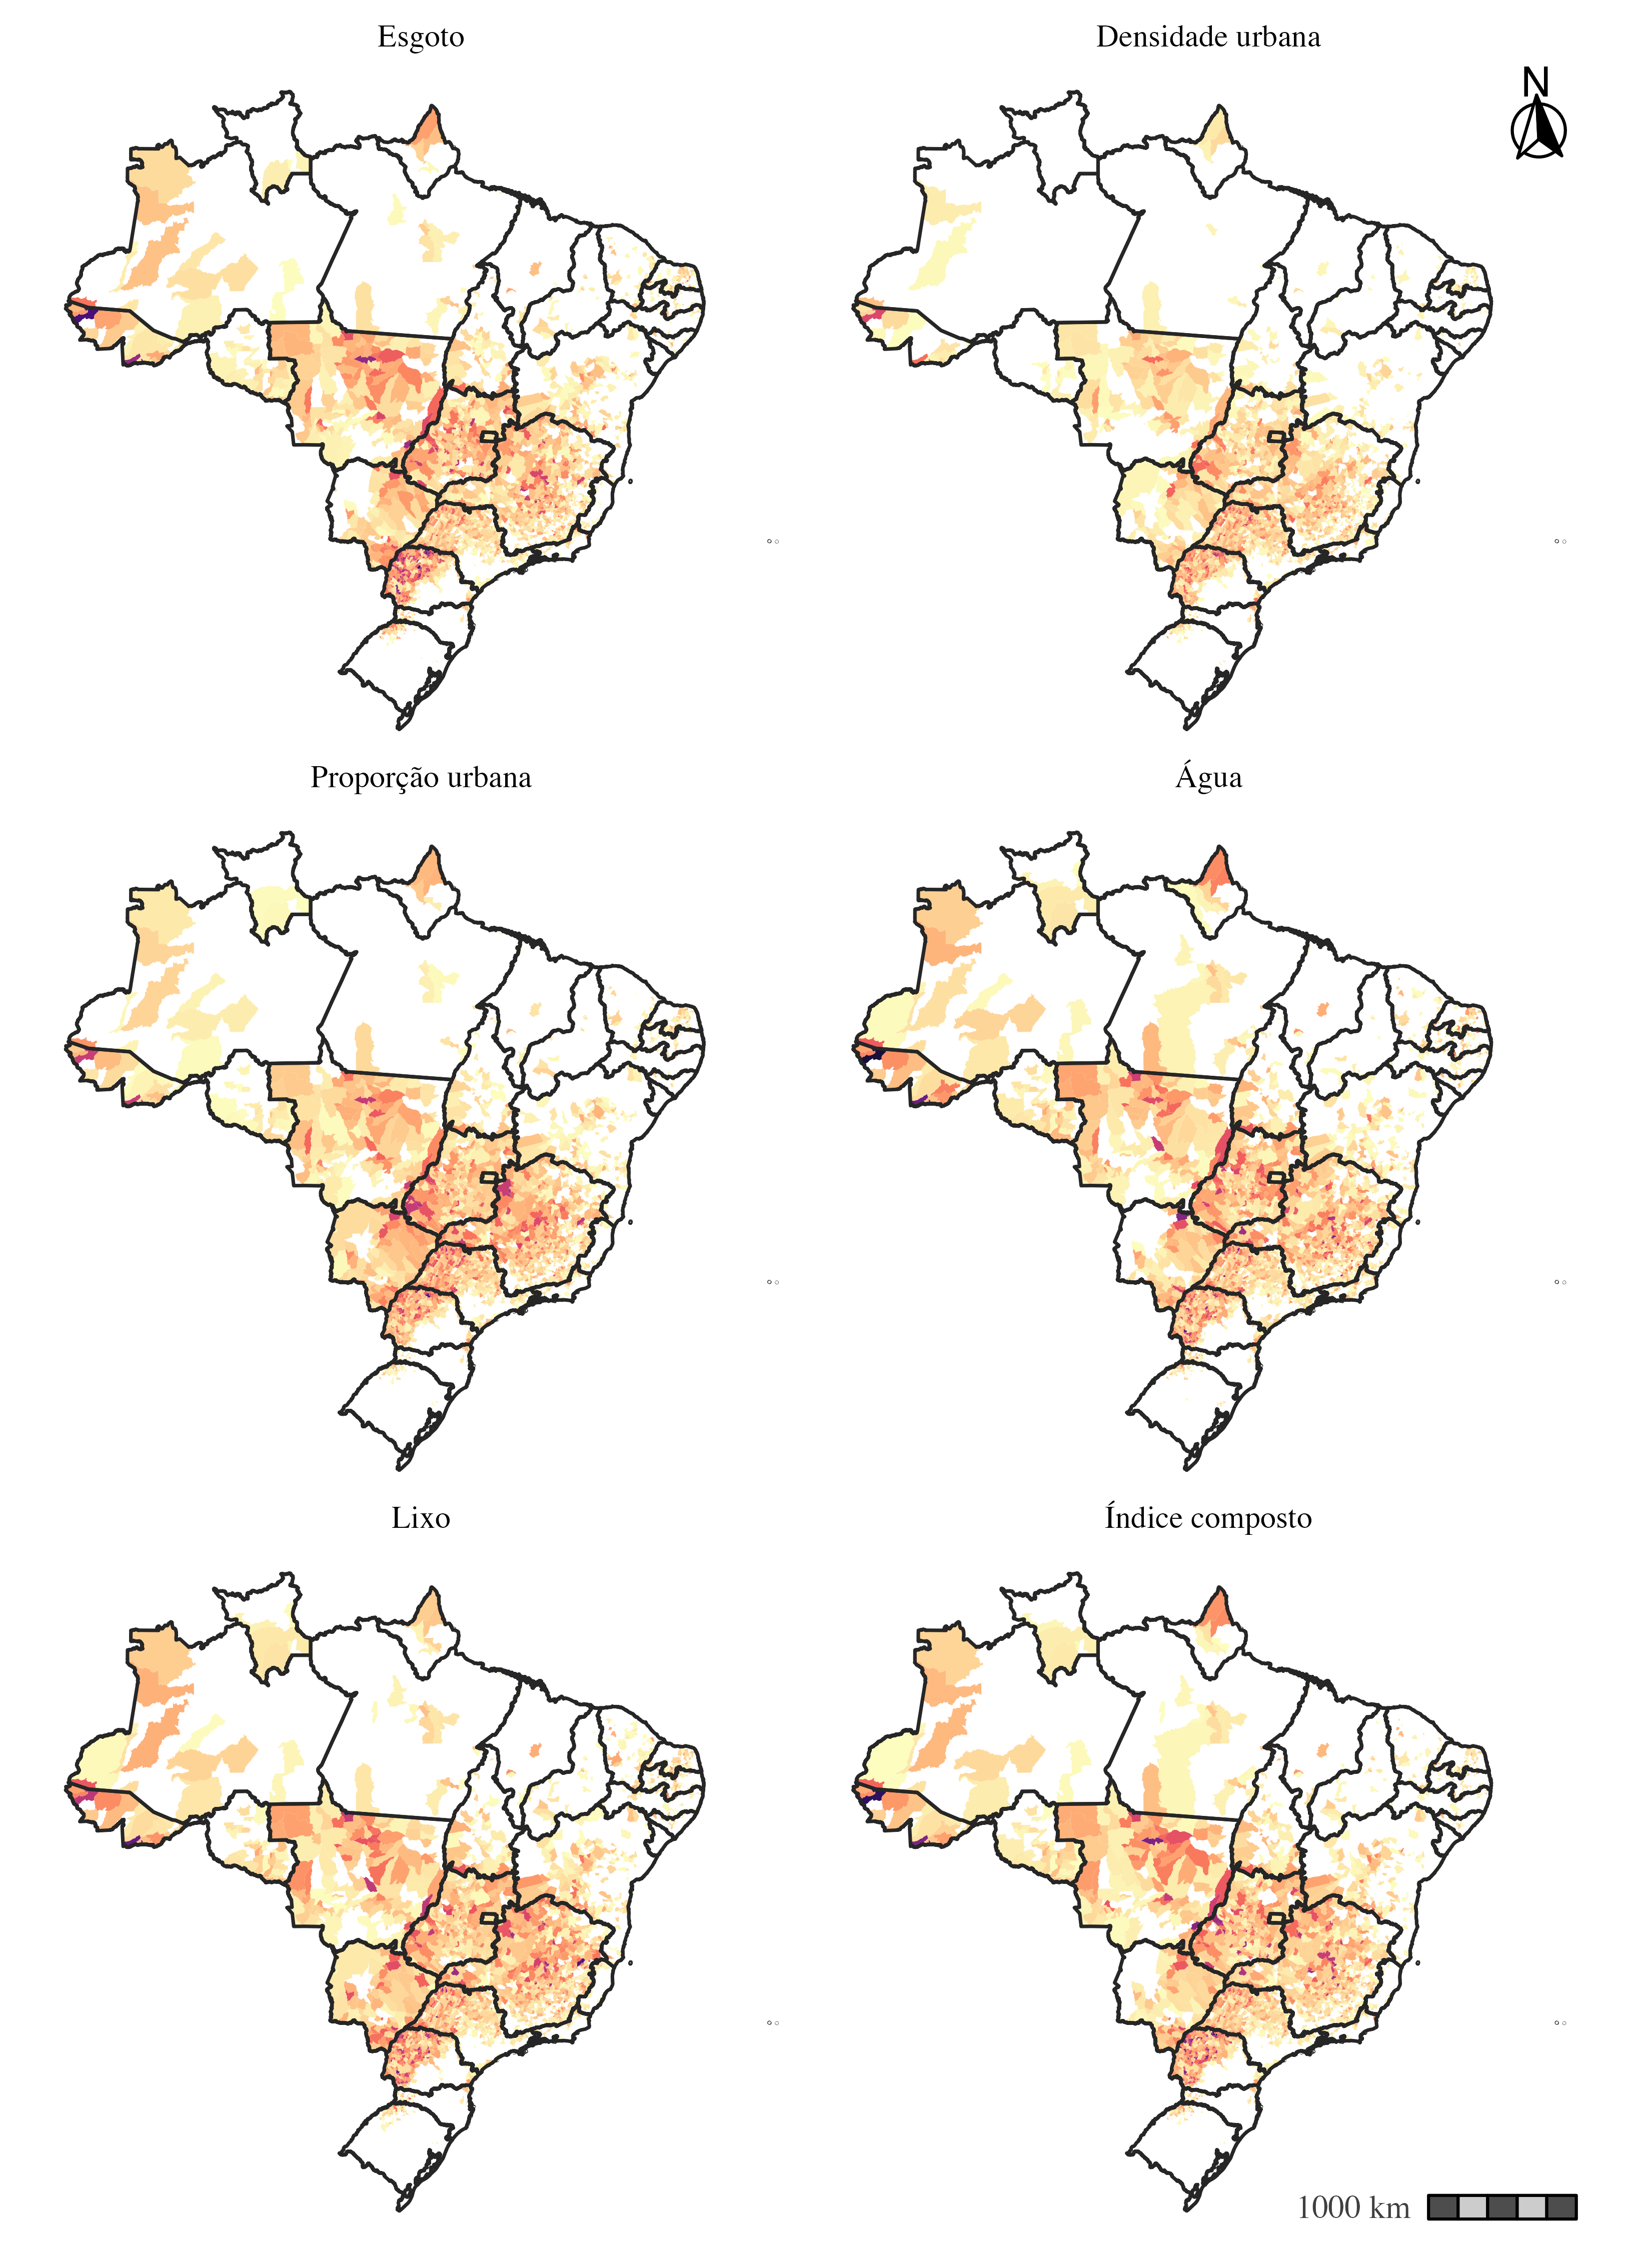
\includegraphics[width=0.86\textwidth]{fig_prancha_rr_completo.png}
    \caption{Risco relativo municipal estimado pela varredura espacial sob os ajustes por esgoto, densidade urbana, proporção urbana, água, lixo e índice composto (ordem de leitura), Brasil, 2010--2025. Fontes: SINAN e IBGE.}
    \label{fig:prancha_rr}
    \vspace{0.3em}
    {\footnotesize\noindent\textit{Nota:} Tons mais escuros indicam risco relativo mais alto, na escala comum às seis formulações, de 1,0 a 11,9; em branco, municípios com $RR \le 1{,}0$. Os dois primeiros modelos constam da Figura~\ref{fig:mapas_rr}.\par}

\end{figure}

\bibliography{referencias}

\end{document}
